%%%%%%%%%%%%%%%%%%%%%%%%%%%%%%%%%%%%%%%%%
% Tufte-Style Book (Minimal Template)
% LaTeX Template
% Version 1.0 (5/1/13)
%
% This template has been downloaded from:
% http://www.LaTeXTemplates.com
%
% License:
% CC BY-NC-SA 3.0 (http://creativecommons.org/licenses/by-nc-sa/3.0/)
%
% IMPORTANT NOTE:
% In addition to running BibTeX to compile the reference list from the .bib
% file, you will need to run MakeIndex to compile the index at the end of the
% document.
%
%%%%%%%%%%%%%%%%%%%%%%%%%%%%%%%%%%%%%%%%%

%----------------------------------------------------------------------------------------
%	PACKAGES AND OTHER DOCUMENT CONFIGURATIONS
%----------------------------------------------------------------------------------------

\documentclass[notoc]{tufte-book} % Use the tufte-book class which in turn uses the tufte-common class
 

\setcounter{tocdepth}{2} 
\setcounter{secnumdepth}{2}

\hypersetup{colorlinks} % Comment this line if you don't wish to have colored links

\usepackage{microtype} % Improves character and word spacing

\usepackage{booktabs} % Better horizontal rules in tables

\usepackage{graphicx} % Needed to insert images into the document
\setkeys{Gin}{width=\linewidth,totalheight=\textheight,keepaspectratio} % Improves figure scaling

\usepackage{fancyvrb} % Allows customization of verbatim environments
\fvset{fontsize=\normalsize} % The font size of all verbatim text can be changed here

\newcommand{\hangp}[1]{\makebox[0pt][r]{(}#1\makebox[0pt][l]{)}} % New command to create parentheses around text in tables which take up no horizontal space - this improves column spacing
\newcommand{\hangstar}{\makebox[0pt][l]{*}} % New command to create asterisks in tables which take up no horizontal space - this improves column spacing

\usepackage{xspace} % Used for printing a trailing space better than using a tilde (~) using the \xspace command

\setlength{\parskip}{0.15cm plus0.5mm minus0.5mm}

\newcommand{\monthyear}{\ifcase\month\or January\or February\or March\or April\or May\or June\or July\or August\or September\or October\or November\or December\fi\space\number\year} % A command to print the current month and year

\newcommand{\blankpage}{\newpage\hbox{}\thispagestyle{empty}\newpage} % Command to insert a blank page

%code structuring
\usepackage{listings}
\usepackage{color}

\definecolor{dkgreen}{rgb}{0,0,0}
\definecolor{gray}{rgb}{0,0,0}
\definecolor{mauve}{rgb}{0,0,0}

\lstset{frame=none,
  language=Python,
  aboveskip=3mm,
  belowskip=3mm,
  showstringspaces=false,
  columns=flexible,
  basicstyle={\small\ttfamily},
  numbers=none,
  numberstyle=\tiny\color{gray},
  keywordstyle=\color{gray},
  commentstyle=\color{dkgreen},
  stringstyle=\color{mauve},
  breaklines=true,
  breakatwhitespace=true
  tabsize=3
}

%----------------------------------------------------------------------------------------
%	BOOK META-INFORMATION
%----------------------------------------------------------------------------------------

\title{An Introduction to TouchDesigner} % Title of the book

\author{Elburz Sorkhabi} % Author

\publisher{nVoid Art-Tech Limited} % Publisher

%----------------------------------------------------------------------------------------

\begin{document}

\frontmatter


%----------------------------------------------------------------------------------------

\maketitle % Print the title page

%----------------------------------------------------------------------------------------
%	COPYRIGHT PAGE
%----------------------------------------------------------------------------------------

\newpage
\begin{fullwidth}
~\vfill
\thispagestyle{empty}
\setlength{\parindent}{0pt}
\setlength{\parskip}{\baselineskip}
Copyright \copyright\ \the\year\ \thanklessauthor

\par\smallcaps{Published by \thanklesspublisher}

\par\smallcaps{\url{hello@nvoid.com}}

\par This work is licensed under the Creative Commons Attribution-NonCommercial-ShareAlike 4.0 International License. To view a copy of this license, visit \url{http://creativecommons.org/licenses/by-nc-sa/4.0/deed.en_US}.\index{license}

\par\textit{First printing, \monthyear}
\end{fullwidth}

%----------------------------------------------------------------------------------------

\tableofcontents % Print the table of contents


%----------------------------------------------------------------------------------------
%	DEDICATION PAGE
%----------------------------------------------------------------------------------------

\cleardoublepage
~\vfill
\begin{doublespace}
\noindent\fontsize{18}{22}\selectfont\itshape
\nohyphenation
Dedicated to 3am nights (hard work) and 4am mornings (perseverence).
\end{doublespace}
\vfill
\vfill

%----------------------------------------------------------------------------------------
%	INTRODUCTION
%----------------------------------------------------------------------------------------

%----------------------------------------------------------------------------------------
%	INTRODUCTION
%----------------------------------------------------------------------------------------

\cleardoublepage
\chapter{Introduction}
\label{introduction}
%------------------------------------------------

\section{Foreword}

\vspace{10mm}

\begin{fullwidth}
Between the artist and the tool are countless techniques and bits of know-how that contribute to the artist becoming more fluid and well-equipped for the challenges of production.
 
When I caught wind of Elburz' TouchDesigner book project, I thought, yes I'd like to know what he knows!
 
Elburz' deep storage of TouchDesigner wisdom was absorbed from multiple sources - helping and conversing with a myriad of users on the forums, red-lining on-the-job on time-critical projects, working with Derivative using beta builds of TouchDesigner, and his purely exploratory endeavors mixed with his side-life as a hip-hop trombonist and VJ.
 
The book is a good keyboard-side or bed-side companion that explores the concepts, techniques and methodology behind TouchDesigner - something I have not had the opportunity to personally present before and am very happy Elburz has presented here. So build your chops with these treats - It can be read end-to-end or by randomly flipping through pages, as I found myself doing - discovering gems of information and insights throughout.
 
Many thanks to Elburz for this initiative to enrich the TouchDesigner community. I'm sure it will trigger a great chain reaction.

\vspace{10mm}

\textit{Greg Hermanovic}

\textit{Founder}

\textit{Derivative}

\clearpage

\end{fullwidth}

%------------------------------------------------

\section{Foreword by Author}

\begin{fullwidth}

\vspace{10mm}

The purpose of this book is two-fold:
\begin{itemize}
\item to teach the fundamentals of TouchDesigner 088
\item to create a community-driven resource for beginners
\end{itemize}

The first purpose is straightforward. We will look at various UI elements, discuss Operators and Operator families, explore logical workflows, Network optimizations, performance interfaces, display management, and etc. TouchDesigner's core elements will be explained and demonstrated, and many common problems will be pre-emptively dealt with.

After the written portion, we will learn how to approach solving a problem with example projects and video tutorials at the end of the book. These lessons will be practical in that we will assemble a few projects and useful modules from the ground up.

The second purpose of this book is slightly more asking of the community. We really believe in the community, so instead of selling this book, we wanted everyone to be able to access it for free (text, video, and example files). We wanted to take this idea a step further, and not only allow free access to the book's contents, but also allow free access to the book's building blocks.

What this means is that anyone can feel free to add, comment, change, mark up, delete, or increment upon the resources in this book. All of the book has been completely written using LaTeX, and the code to compile the book, project files, examples, diagrams, and videos, and whatever else ends up within it, will all be hosted on GitHub, and will be free (under a Creative Commons license) for anyone to download, share, and build upon.

For quality control purposes, everyone will be able to branch the repository, but we will review all changes before integratating updates back into a main branch. Everyone who contributes will be thanked and added to the 'Credits' portion of the book. This way, a new user only has to look for a single PDF, or download link, to receive the communities most up-to-date knowledge.

We really hope that the community engages with this and helps create the ultimate how-to resource for beginners!

As of the initial writing, knowing what this book is will be as important as knowing what this book is not. This book is not an Operator reference manual. We will not cover every parameter or use of every Operator. This book is not meant to replace the Derivative Wiki as the main reference, we will only use and learn about what we need. This book is not meant to replace the forum's wealth of helpful users and components.

In the end, this resource is a tribute to many TouchDesigner programmers and Derivative staff who, whether on the forum, or in real-life, have helped all of us get where we are. We hope that this tradition will continue as long as TouchDesigner does. 

\vspace{10mm}


\textit{Elburz Sorkhabi \& nVoid Art-Tech Limited}

\end{fullwidth}

%------------------------------------------------
\vspace{15mm}
\section{What is TouchDesigner?}
\begin{fullwidth}

This is a question many users spend time trying to answer when starting out. It can be surprising how long it takes to create and perform simple tasks. It can be surprising that a good amount of time is spent building functionality that is already native to other software packages. So what is TouchDesigner? The answer is simple: TouchDesigner is a visual, node-based programming language.

Starting from possibly the most important aspect of the description, TouchDesigner is a programming language. TouchDesigner isn't an application that is ready on start to perform actions that may seem simple in other applications. TouchDesigner is an environment with extreme depth, and many potential pitfalls. With some practice and time, many things can be created quickly as theyre required. With the book's goal to create re-useable modules, the speed at which a blank canvas can become a finished project will be greatly increased. This doesn't negate the fact that TouchDesigner is still a programming language. Many tasks will still require due diligence in regards to time and effort. Many will require quite a bit of head-scratching, and all of them will require some basic problem-solving skills. 

The second aspect of the description is that TouchDesigner is node-based. This mean that instead of opening a text document and typing line after line of code, TouchDesigner's graphical interface is used to make applications out of nodes. Each node, or Operator in TouchDesigner, performs a specific, small, and granular action. To perform complex tasks, a handful of nodes will work together. To send information between these nodes, their inputs and outputs are wired together. There are many node-based programming languages in existence, such as Cycling 74's Max/MSP, but what sets TouchDesigner apart is it's visual nature.

Everything in TouchDesigner has a visual counterpart. All the Operators have viewers. Everything, whether it be text, control data, audio, videos, and more, is visualized through each and every operation that is performed. This is unlike any traditional programming, and even node-based, language, but it is what makes TouchDesigner a fantastic environment to work with. Learning how to do many complex tasks is greatly simplified by the ability to visualize the steps involved, every step of the way. 

\end{fullwidth}
%----------------------------------------------------------------------------------------


\mainmatter
%----------------------------------------------------------------------------------------
%	CHAPTER 1
%----------------------------------------------------------------------------------------

\cleardoublepage
\chapter{Basics}
\label{ch:1}

%------------------------------------------------

\section{Signal Flow and Wiring}

\begin{fullwidth}
Wiring Operators is the most basic operation in TouchDesigner. All projects are made up of nothing more than groups of Operators wired together. Each Operator, on its own, does a very specific thing, but when they are combined together into a 'Network', they can solve extremely complex problems.

All data in TouchDesigner flows from left to right. Any inputs that an Operator has will always be on the left side, and outputs will be on the right side. The inputs and outputs will also be ordered first to last, going from top to bottom. In the example diagram below, follow the two signals starting on the left. As they flow from left to right, they are composited, one over the other.

\begin{center} 
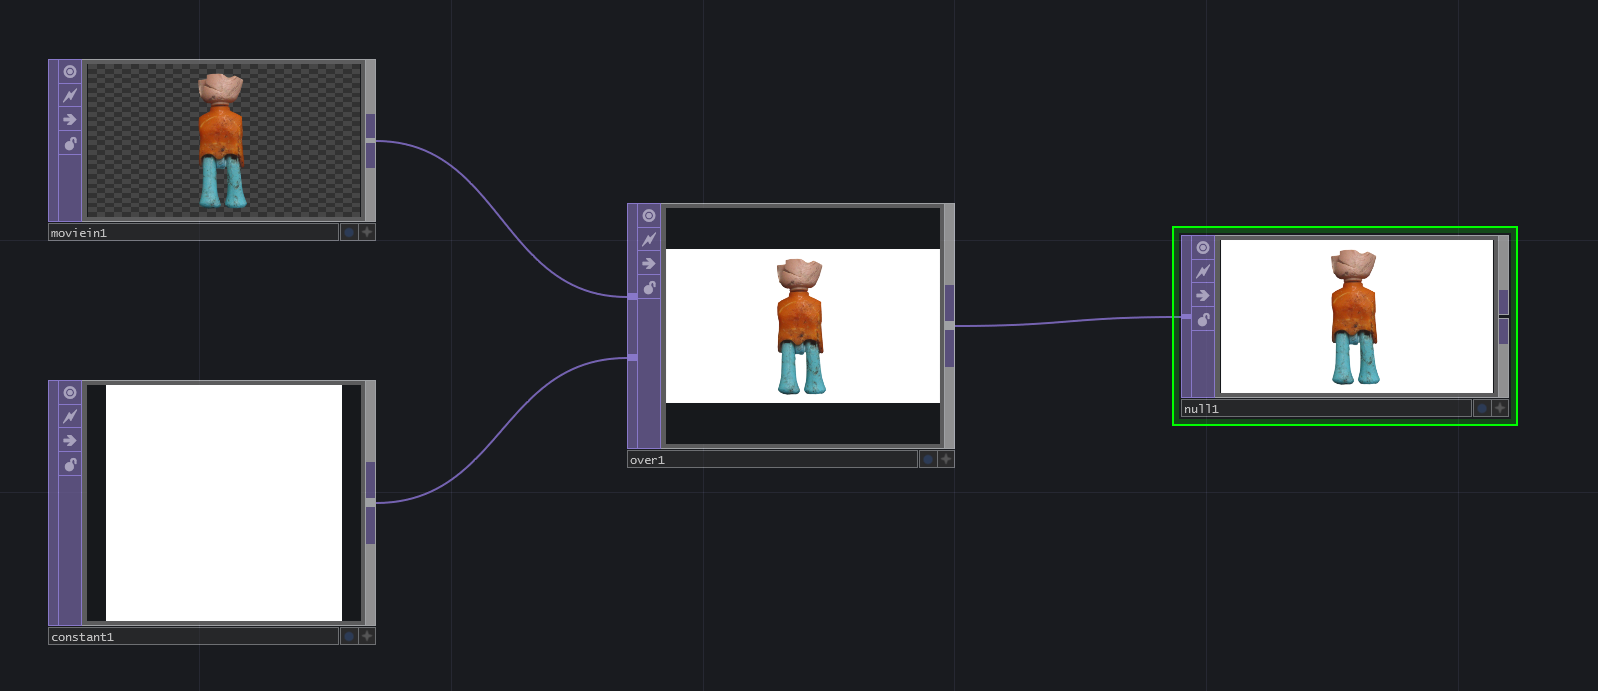
\includegraphics{./img/1.1/signal-flow-1.png}
\end{center}

Components, interestingly, have the same data signal flow as Operators, flowing from left to right, but they are also capable of parent and child relationships, which flow from top to bottom. The component at the top of the signal chain is the parent, and the components below it are its children, and below that are the children's children, and so on. In the example below, there is a small UI, that is made of a few sliders. In this example, the Slider COMPs are the children of the Container COMP, which is the parent.

\begin{center} 
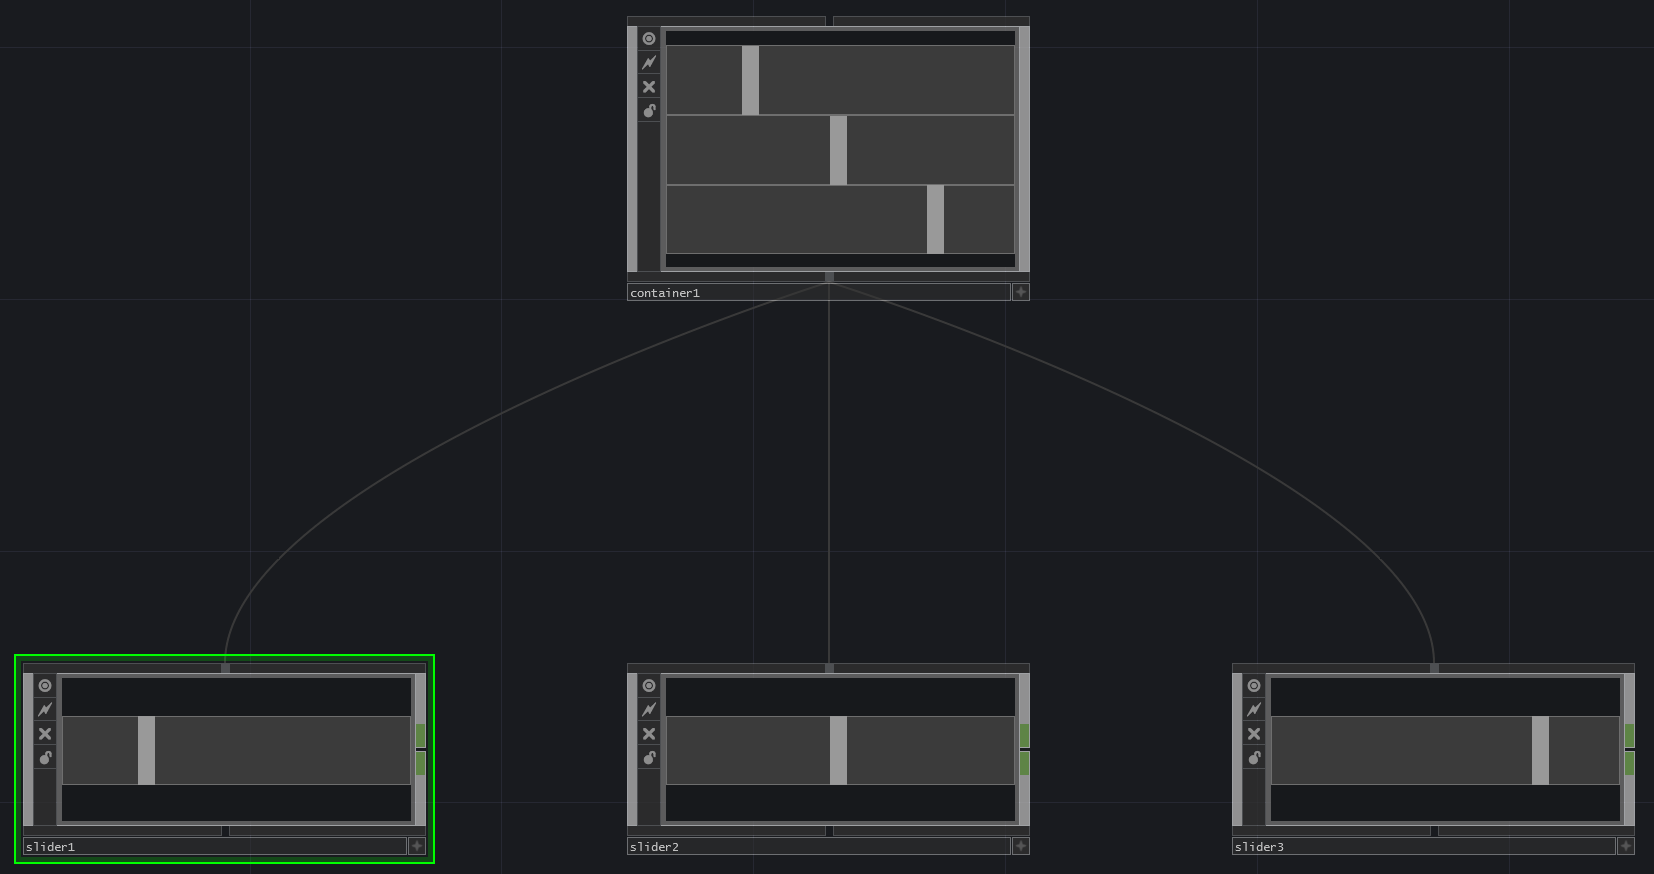
\includegraphics{./img/1.1/signal-flow-2.png}
\end{center}

\end{fullwidth}

%------------------------------------------------

\section{Creating Operators}
\begin{fullwidth}
The OP Create dialog can be reached in a multitude of ways. Each has a correct time and place of usage. When creating Operators from scratch the two easiest methods are to hit 'Tab' on the keyboard, or to double click on the Network background.

When working with existing chains of Operators, there are two easy ways to add Operators. The first is to right click on either the input or output of an Operator. This will add the chosen Operator, pre-wired, directly before the input or after the output. This is especially useful as it inserts the Operator seamlessly into a pre-existing chain.

For example, there is a Constant TOP wired to a Null TOP, and a Transform TOP needs to be added between the two. Right clicking either the output of the Constant TOP, or the input of the Null TOP, and selecting Transform TOP, would create a Transform TOP, that would be pre-wired in-between the Constant TOP and Null TOP.

Similar results can be achieved by right clicking on the wire itself and clicking on 'Insert Operator'. This would similarly create and pre-wire the chosen Operator between the two existing Operators.

The third way to add an Operator to an existing chain is to right click on a wire itself, and click  'Add Operator'. The difference between 'Insert Operator' and 'Add Operator'  is that inserting an Operator integrates it into the current Operator chain, whereas adding an Operator creates the Operator and wires it in parallel to the wire that is right clicked on. 

In the diagram below, there is an example with a Constant TOP and a Null TOP. In the next diagram, the wire connecting them was right clicked and a Transform TOP was created using 'Insert Operator'. In the proceeding diagram, the wire connecting the Operators was right clicked and a Transform TOP was created using 'Add Operator'. Notice how it is pre-wired in parallel to the first Transform TOP.


\begin{center} 
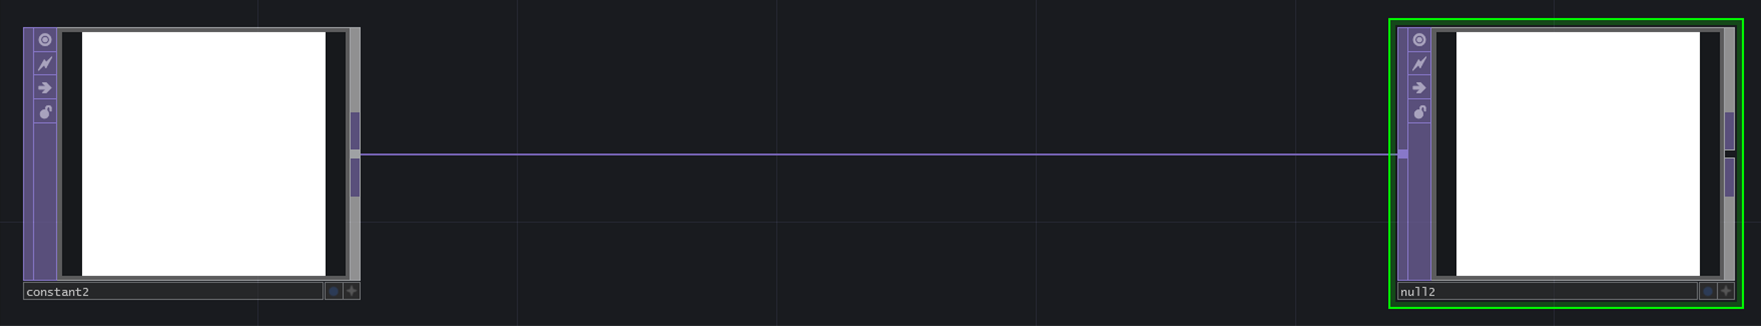
\includegraphics{./img/1.2/creating-operators-1.png}

\center 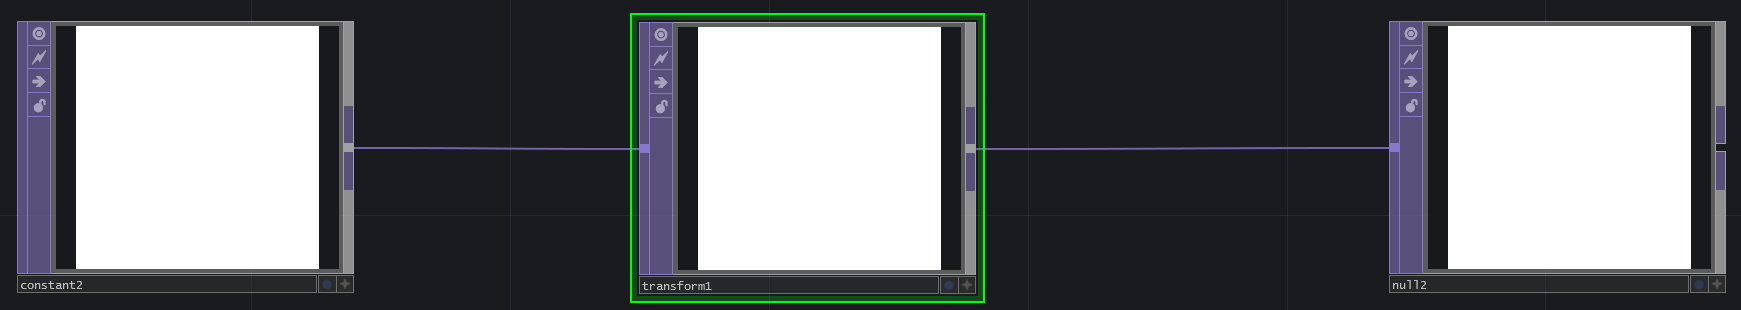
\includegraphics{./img/1.2/creating-operators-2.png}

\center 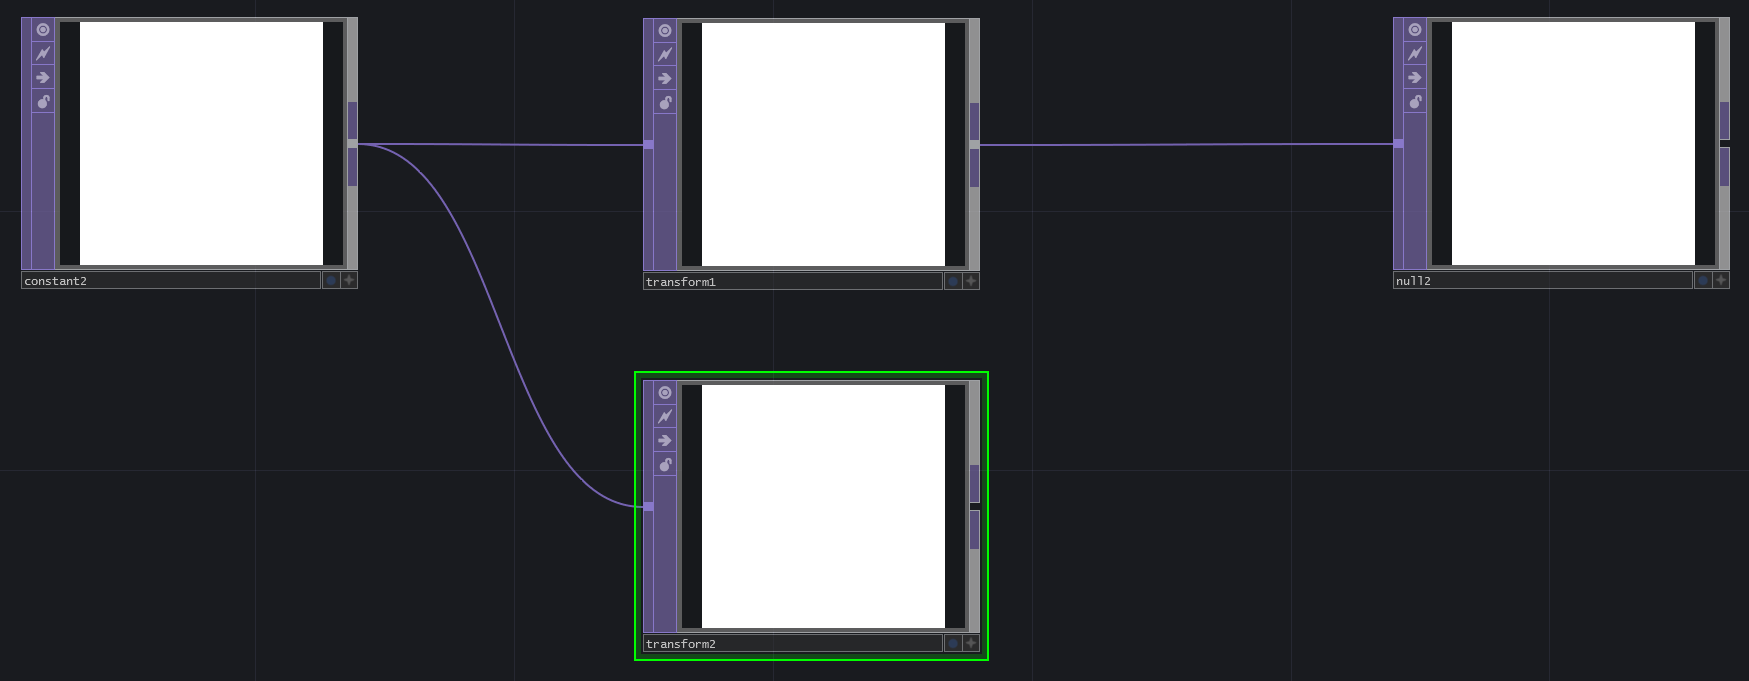
\includegraphics{./img/1.2/creating-operators-3.png}
\end{center}

There are two useful key commands when working with the OP Create Dialog: 'Control' and 'Shift'. Open the OP Create dialog, hold down 'Control' on the keyboard, and then begin to select multiple Operators in a row. Each one will be added to the Network below the last. This is useful for quickly populating a Network with a few different Operators. 

Similarly, open the OP Create dialog, press and hold the 'Shift' key, and then begin to select multiple Operators. This is different than above, in that the Operators will be wired together in series. This key command can be used to quickly create small, or large, chains of pre-wired Operators. 

Both of these key commands are quite powerful, but they become even more so when they are used in tandem. For example, a project requires 3 chains of Operators. The first will consist of a Circle TOP, connected to a Blur TOP, connected to a Null TOP. The second will consist of a Circle TOP, connected to an Edge TOP, connected to a Noise TOP, connected to a Null TOP. The final chain will consist of a Movie In TOP, connected to a Blur TOP, connected to a Null TOP. Let's go through this step by step, to demonstrate practical use of the above key commands:

\begin{enumerate}
\item Open the OP Create dialog
\item Press and hold down 'Shift'
\item While holding 'Shift', click on Circle TOP, Blur TOP, then Null TOP. This will create the first chain.
\item Release the 'Shift' key 
\item Press and hold down 'Control'. This will place the next Operator below the first Operator.
\item Holding 'Control', click on Circle TOP
\item Release the 'Control' key
\item Press and hold down the 'Shift' key
\item While holding 'Shift', click on Edge TOP, Noise TOP, and then Null TOP. This will create the second chain 
\item Release the 'Shift' key
\item Press and hold 'Control'
\item While holding 'Control', click on Movie In TOP. 
\item Release the 'Control' key
\item Press and hold 'Shift' 
\item Click on the remaining operators: Blur TOP, and Null TOP
\item Now that all of the Operators are created, use the 'Esc' key to close the OP Create dialog.
\end{enumerate}

After closing the OP Create Dialog, all the required Operators will be wired and ready to go in the project. These key commands have not only saved having to open and close the OP Create Dialog for every Operator, but they've saved the need to manually wire them.

\end{fullwidth}

%------------------------------------------------

\section{Mouse and Keyboard Navigation}
\begin{fullwidth}
The mouse plays a vital role in TouchDesigner programming, and a high-quality mouse is highly recommended. The mouse is used to move around the Network and work with Operators. 

Left click on an Operator to select it. Left click and drag that Operator to move it around the Network. To navigate around the Network, left click and drag the Network background. Right click on an Operator to reveal a menu with options that will be introduced slowly. To select and work with more than one Operator, right click and drag the selection box around the desired Operators. Middle click on an Operator to get more info about it. There is a UI button that displays the same Operator info window, which is useful when using a mouse that doesn't have a middle click button.

\begin{center}
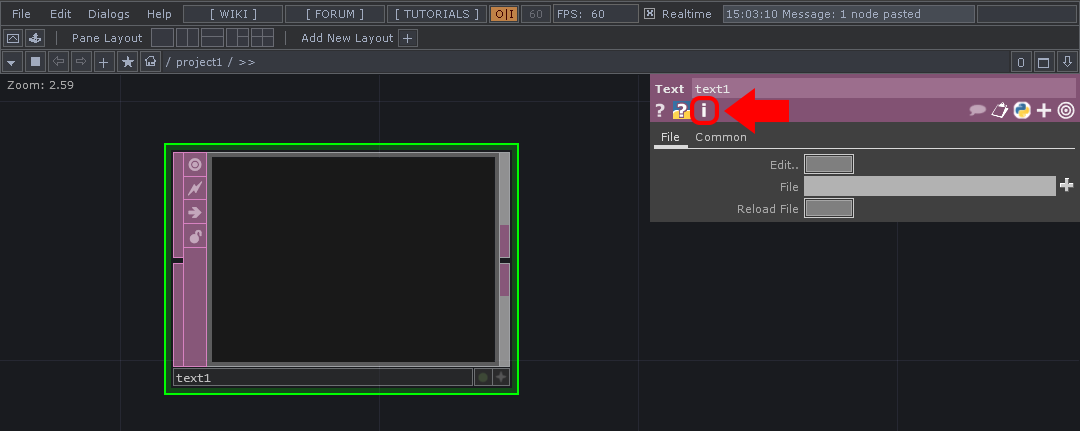
\includegraphics{./img/1.3/navigation-1.png}
\end{center}

Click on the 'i' to get more detailed information about the selected operator.

There are several key commands used to navigate TouchDesigner projects. Two of these key commands are 'u' and 'i'. Press 'u' will move up one Network, and out of the current component. To go inside of a Network or component (like a Container COMP or Base COMP), select the component and hit 'i'.

To centralize the screen on all the Operators in a Network, use the 'h' key on the keyboard. This performs the 'Home' action on the current Network. 

\end{fullwidth}

%------------------------------------------------

\section{Networks and Paths}
\begin{fullwidth}
All TouchDesigner projects are made of Networks. A Network is a group of Operators. Networks are encapsulated inside of components, such as a Container COMP, Base COMP, Geometry COMP, etc. Networks can be infinitely nested. The top level is called the 'root' level. TouchDesigner system and UI elements can be found at the 'root' level.

Encapsulating and organizing Networks from the start of the project is a great practice to get in the habit of. The current path is always visible in the 'Path Bar' at the top of the 'Network Editor'.

\begin{center}
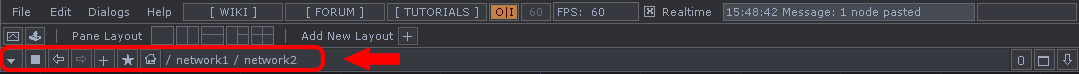
\includegraphics{./img/1.4/path-1.png}
\end{center}

All TouchDesigner Operators have a path. These paths are similar to Unix file paths. There are two kinds of paths to an Operator: the 'absolute path' and the 'relative path'. The 'absolute path' is the path to the Operator from the 'root' of the project, or '/'. The 'relative path' is the path to an Operator from another Operator. These paths start from the Network of the referencing Operator, instead of starting from the 'root'.

Open example 'Paths.toe'. This example demonstrates paths. TouchDesigner will start in the 'root' of the project where there is a Container COMP named 'network1'. Inside of 'network1', there are two Operators. 'rel1' is a Text DAT with two paths in its contents. The first is an 'absolute path'. This path starts from the 'root', or top of the project, and travels towards the Operator. The second path is the 'relative path' from the current Operator to 'rel2', which is a Text DAT inside of the Container COMP named 'network2'. In the 'relative path', the path travels from the current location to the destination. To get from 'rel1' to 'rel2', the path only needs to travel into 'network2', thus the 'relative path' is 'network2/rel2'.

Notice that the viewer of 'network2' is displaying an Operator from inside of it. This technique will be discussed more in later examples, but what is important now is the path used. In the 'Operator Viewer' parameter of 'network2', there is the path to './display', where 'display' is the name of the Operator, and './' denotes one level inside of the referencing Operator, which is 'network2' in this case. 

Inside of 'network2', there is a Text DAT named 'display', whos contents are being displayed in the Network above. The other two Text DATs have more path examples written in them. 'abs1' is another example of an 'absolute path'. 'rel2' has an example of a 'relative path' between itself and 'abs1'. It also has an example of a 'relative path' between itself and 'rel1' in the Network above, where 'rel1' is the Operator's name, and '../' denotes one Network level above the current Network. '../' can be used in sequence to move up as high as the root, but there are more efficient ways of making paths.


\end{fullwidth}

%------------------------------------------------

\section{Using an External Text Editor}
\begin{fullwidth}

Small Python scripts can be created and edited inside of TouchDesigner, but as scripts grow, an external text editor can save a lot of time and trouble.

There are a number of helpful features gained by editing scripts in an external text editor. Without creating an extensive list, some reasons include:

\begin{enumerate}
\item Line numbering 
\item Colour coded syntax
\item Find \& Replace functionality
\item Auto-completion
\end{enumerate}

These features add up to a far richer, and more efficient experience when working extensively with Python inside of TouchDesigner.  

To setup an external editor the steps are as follows:

\begin{enumerate}
\item Open the 'Preferences' dialog found in the 'Edit' menu
\item Go to the 'DATs' preferences
\item Click the file browser icon for the 'Text Editor' setting
\item Assign the the external editor's executable (.exe) by selecting it and clicking 'Open'.  This is usually located in the 'Program Files' folder
\item Click 'Accept' on the Preferences dialog
\end{enumerate}

Once the setup is complete, right click on a DAT and click the 'Edit Contents' option. The DAT will be opened in the program which is specified by this preference.  A separate 'Table Editor' preference is available to set the external editor used for DATs that are tables.

Two well-respected editors that are used frequently in the TouchDesigner community, and are cross-platform, are linked below: 

\begin{description}
\item[Sublime Text 3] \url{http://www.sublimetext.com/}
\item[Notepad++] \url{http://notepad-plus-plus.org/}
\end{description}

\end{fullwidth}
%------------------------------------------------

\section{Help}

\begin{fullwidth}

If there are ever any questions about specific Operators or processes, refer to the official Derivative Wiki. Each Operator has two shortcuts that will open it's Wiki page in a new browser window. These two buttons are located in the Parameter window, and both are represented by question marks. One is specifically about the Operator and it's use, while the other, the question mark over the Python logo, is specifically about Python scripting with that Operator.

\begin{center}
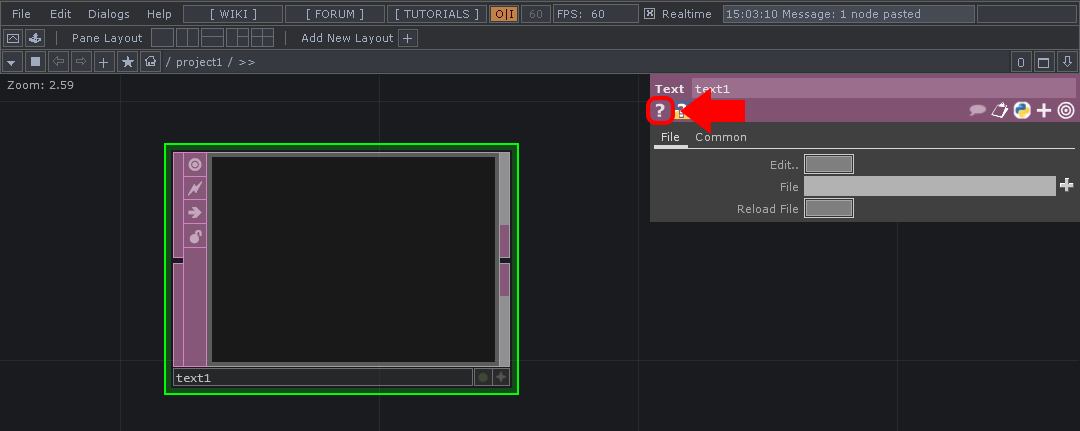
\includegraphics[width=15cm]{./img/1.6/help-1.png}

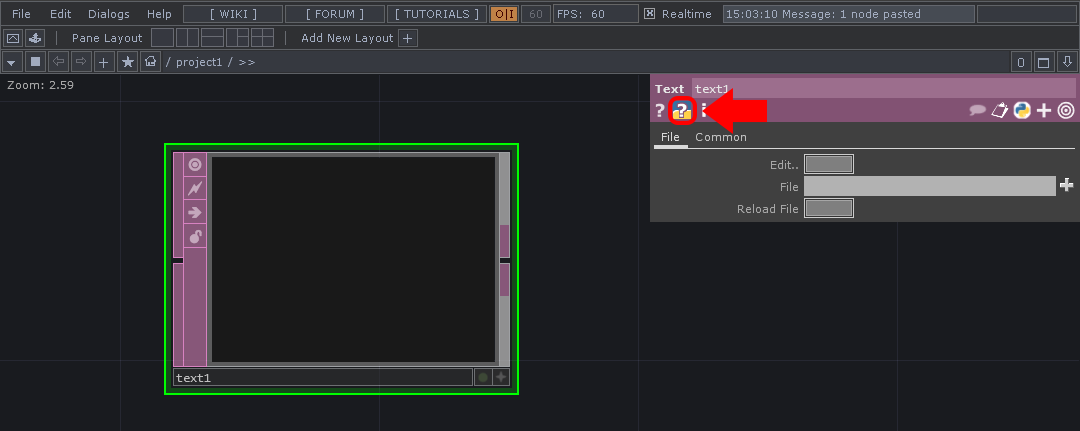
\includegraphics[width=15cm]{./img/1.6/help-2.png}
\end{center}

\end{fullwidth}

%------------------------------------------------



%----------------------------------------------------------------------------------------
%	CHAPTER 2
%----------------------------------------------------------------------------------------

\cleardoublepage
\chapter{User Interface}
\label{ch:2}

%------------------------------------------------
\section{Parameter Window}

\begin{fullwidth}

The 'Parameter Window' is where all an Operator's parameters can be accessed.

There are two ways to access the 'Parameter Window'. The first is using the 'P' key. This will open a docked 'Parameter Window' in the top-right hand corner of the pane. This docked 'Parameter Window' will display the parameters of whatever Operator is selected.

The second way to access the 'Parameter Window' is by right clicking on an Operator and selecting 'Parameters...'. This will open up a floating 'Parameter Window' for the Operator. This method differs from the first in that the parameters will not change if another Operator is selected. This is useful for being able to manage the parameters of multiple Operators simultaneously.

Every Operator has a different set of parameters, but all 'Parameter Windows' have the same set of options. Below is a diagram highlighting the options:

\begin{center}
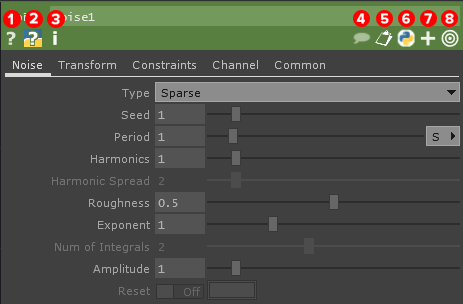
\includegraphics[width=13cm]{./img/2.1/parameter-window.png}
\end{center}

From left to right, the options are as follows:

\begin{enumerate}
\item Operator Help: opens the Operator's Wiki help page in a new browser window
\item Operator Python Help: opens the Operator's Python Wiki help page in a new browser
\item Operator Information Dialog: displays information about the Operator's process, similar to middle-clicking an Operator
\item Comment: display and edit Operator comments
\item Copied Parameters: displays parameters copied via the right click menu
\item Language: choose whether the Operator will use Python or tscript as its scripting language
\item Expand/Collapse Parameters: expand or collapse all the Operator's parameters
\item Non-default Parameters: display only parameters that have been changed from their default values
\end{enumerate}

\end{fullwidth}
%------------------------------------------------
\section{Parameters}

\begin{fullwidth}

Parameters can be entered in a number of ways. Depending on the situation, some parameters may require a static value, and some may need to be driven by other values and inputs. Each parameter has three modes. Each mode is quite different and each defines how the parameter behaves. The three modes are:

\begin{enumerate}
\item Constant mode
\item Expression mode
\item Export mode
\end{enumerate}

Constant mode is the default for most parameters, and is represented by a grey colour scheme in the value field. Expression mode is used for Python, tscript, or mathematical operations and scripts. Expression mode is represented by a dark grey and light blue colour scheme. Export mode is used to directly reference CHOP channels.  It is represented by a light green colour scheme.

Each of an Operators parameters can be independently changed between the three modes. To change the mode of a parameter, hover the mouse over the parameter's name. A '+' sign will appear near the parameter's name, similarly to the diagram below.

\begin{center}
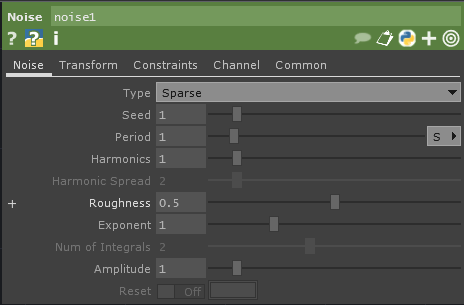
\includegraphics[width=12cm]{./img/2.2/parameters-1.PNG}
\end{center}

Once hovering over the parameter's name, click it and it will expand, displaying more information and options, similarly to the diagram below:

\begin{center}
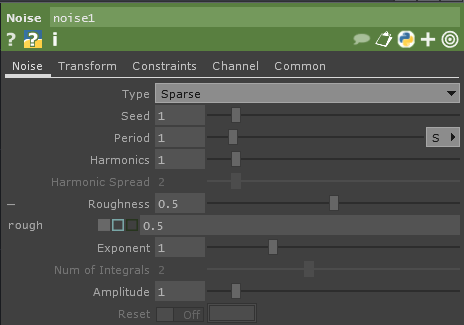
\includegraphics[width=12cm]{./img/2.2/parameters-2.PNG} 
\end{center}

There are three main elements that are available once a parameter is expanded. The first on the left, is the parameter's scripting name. This scripting name is needed whenever that parameter is referenced in any of TouchDesigner's scripting languages. In the above diagram, the scripting name for the Noise CHOP's Roughness is 'rough'. Continuing the above example, the Python script to set the Roughness of the above Noise CHOP to '1' would be:

\begin{lstlisting}
op('noise').par.rough = 1
\end{lstlisting}

The second element is the three coloured squares. These squares represent the different modes for the parameter, as discussed above. Operator parameters set to Constant mode are represented by a filled grey square. This parameter can be changed to Expression mode by clicking on the outline of the light blue square. Once clicked, the light blue square will be filled, and the value field to the right will also be coloured to reflect the parameter's mode.

\begin{center}
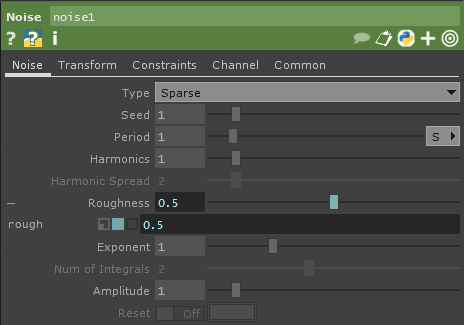
\includegraphics[width=12cm]{./img/2.2/parameters-3.PNG}
\end{center}

To change the parameter's mode to Export mode, a CHOP channel needs to be dragged and dropped on the parameter, at which point it will take up Export mode's colour scheme, and the green box will be filled in.

\begin{center}
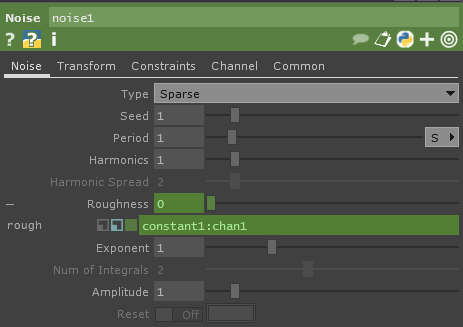
\includegraphics[width=12cm]{./img/2.2/parameters-4.PNG}
\end{center}

The third element of the expanded parameter is the value field. The value field displays a different piece of information depending on the parameter mode. In Constant mode, the value field displays the current value, and can be edited by clicking and typing in the field. In Expression mode, the value field displays the script of Python or tscript that is being evaluated. The expression can be edited by clicking and typing in the value field. In Export mode, the value field displays two pieces of information separated by a colon. The text before the colon displays the path of the CHOP that is exporting to this parameter. The text after the colon is the name of the channel being exported from the CHOP. Because these values are being imposed by another Operator, the value field cannot be edited while the parameter is in Export mode.

\end{fullwidth}
%------------------------------------------------
\section{Transport Controls}

\begin{fullwidth}

The transport bar functions similarly to the transport bars of many other applications. To go through it quickly, from left to right the buttons do the following:

\begin{center}
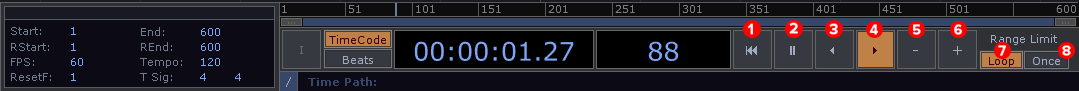
\includegraphics{./img/2.3/transport-1.png}
\end{center}

\begin{enumerate}
\item Resets timeline to frame 1
\item Pause the timeline
\item Play timeline in reverse
\item Play timeline forward
\item Step one frame backward
\item Step one frame forward
\item Setting 'Range Limit' to 'Loop' will continuously loop the timeline
\item Setting 'Range Limit' to 'Once' will play through the timeline and hold the last frame
\end{enumerate}

The most used functions of the timeline are 'Play' and 'Pause', which can be accessed quickly by pressing the 'Space bar' on the keyboard.

\end{fullwidth}
%------------------------------------------------
\section{Timeline Settings}

\begin{fullwidth}

Unless media or animations is locked to the timeline, the 'Timeline settings' won't need to be regularly accessed. The 'Timeline settings' can be found in the bottom left of the window. The key things to know about this area are that the project's 'FPS' and 'Tempo' can be changed here. The project's 'FPS' determines the rate at which the project will render frames. By default it is set to 60 FPS, meaning that TouchDesigner will try to render 60 frames every second. The 'Tempo' will set the BPM (beats per minute) of the project, for use by the Beat CHOP. 

The 'Timeline settings' are use more in situations where animations and media need to be locked to a consistent timeline. The frame controls include 'Start' and 'End', which control the start frame and end frame of the timeline, as well as 'RStart' and 'REnd', which control the loop start and loop end of the timeline. With these settings, it is possible to create an animation that spans the entire timeline, which could be 4000 frames, while still leaving the option to loop a small section of the timeline to work within. 

\begin{center}
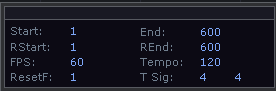
\includegraphics[width=8cm]{./img/2.4/timeline.png}
\end{center}

\end{fullwidth}
%------------------------------------------------
\section{Panes}

\begin{fullwidth}

Using panes regularly can save a ton of time when moving back and forth between Networks. Having to travel through 3 Networks to change a parameter, only to have to travel back to see the changes is a waste of time. Panes take the current window, split it horizontally or vertically as many times as desired. Each pane layout can be saved for later use. 

\begin{center}
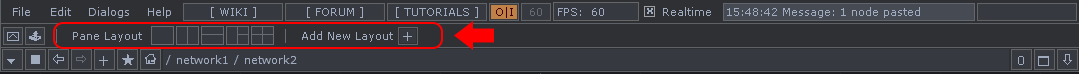
\includegraphics{./img/2.5/panes-1.png}
\end{center}

The diagram above highlights the pane presets that are available by default. The presets provide quick access to a few standard configurations of panes including split left and right, split top and bottom, a 3 pane setup, and a 4 pane setup. Saving pane presets is as easy as clicking the 'Add New Layout +' button, entering a name, and clicking 'Ok'. Saving a layout not only saves the size and position of the panes, but also saves each pane's type. 

Panes are able to display unique types of content, whether they are other dialogs, Networks, or viewers. Being able to mix and match combinations of viewers and Network editors allows for a lot of flexibility. In the diagram below, the top left pane is a Network editor. On the right-hand side, is a Textport, and on the bottom-left, there is a Geometry Viewer. Again, saving this layout would not only save the pane arrangement, but also the pane types. This is useful when working on a project with a lot of different elements, where jumping between something like the setup above, and a simple Network editor, can save quite a bit of time in the long run.

\begin{center}
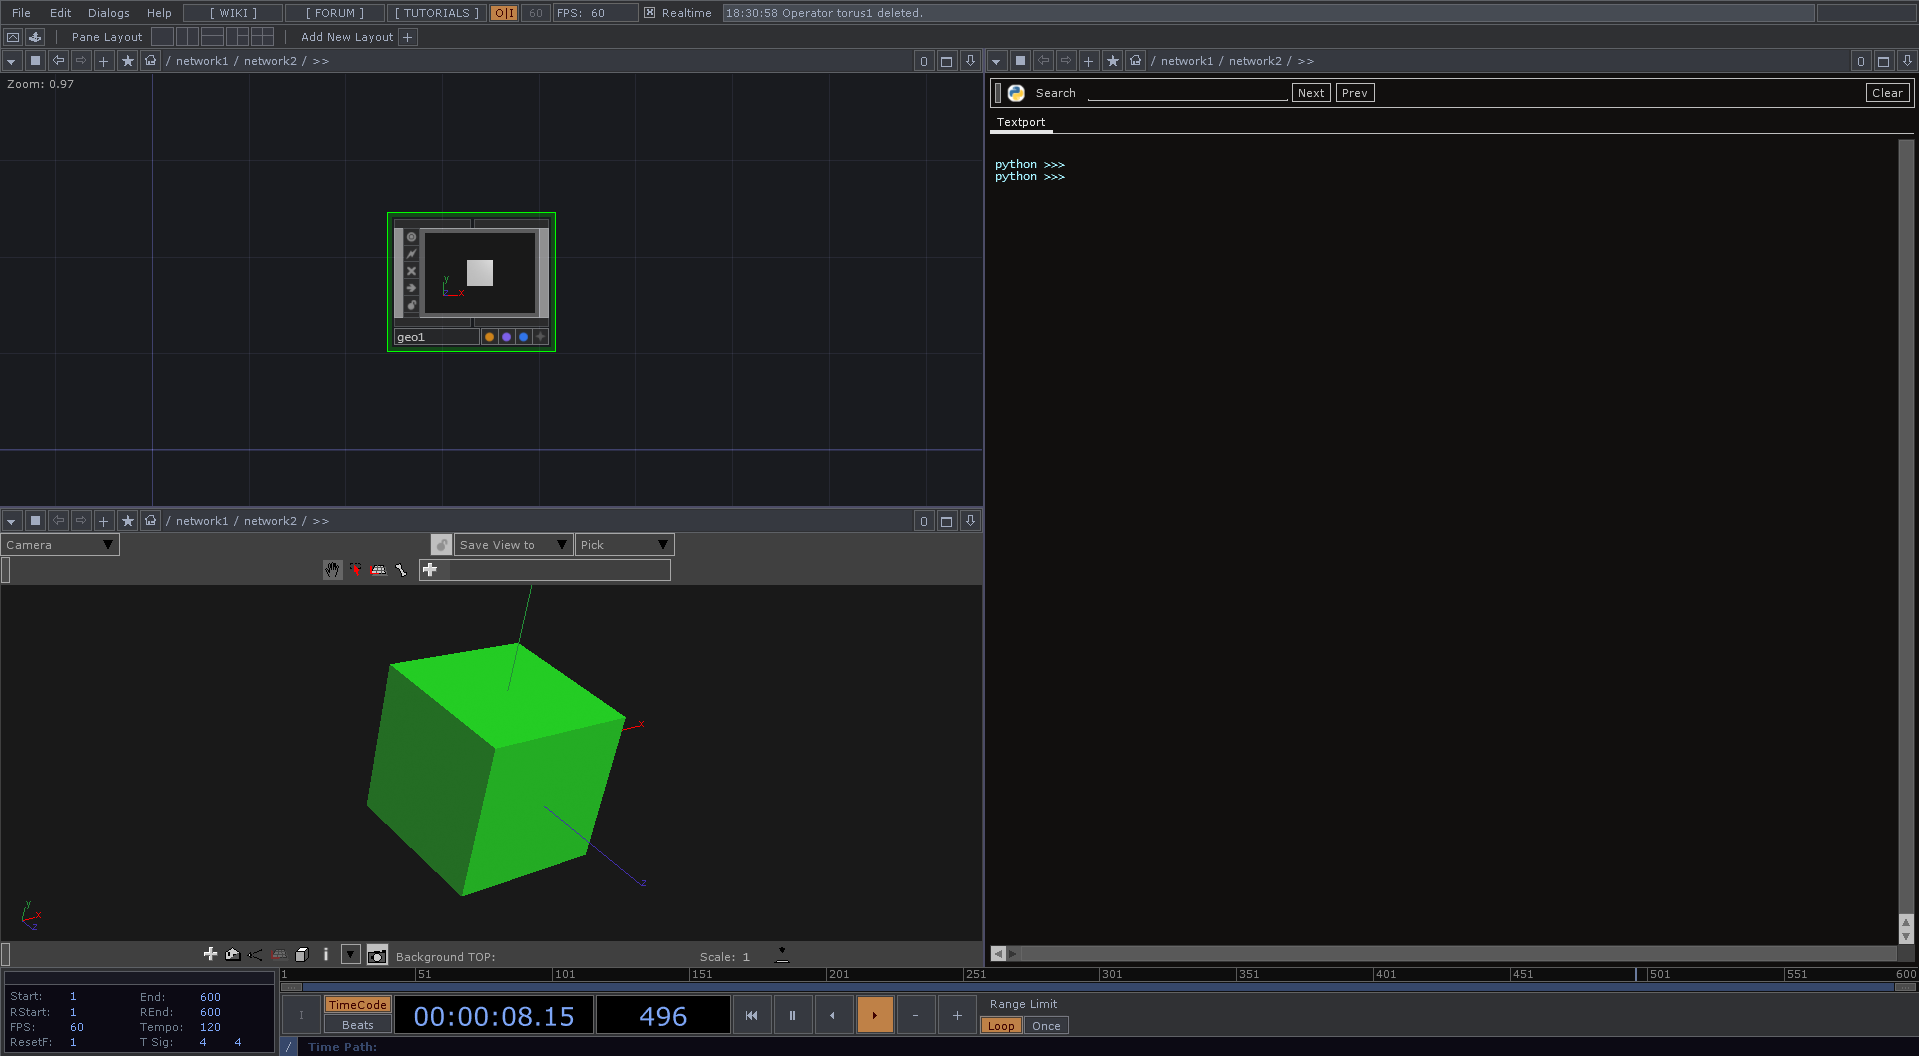
\includegraphics{./img/2.5/panes-2.png}
\end{center}

The keyboard shortcuts for working with panes are as follows:

\begin{itemize}
\item Alt + [ : Vertically split current pane under mouse
\item Alt + ] : Horizontally split current pane under mouse
\item Alt + Z : close pane under mouse
\end{itemize}

\end{fullwidth}
%------------------------------------------------
\section{Palette Browser}

\begin{fullwidth}

The Palette Browser can be thought of as a component library. The Palette Browser holds '.tox' files (or TouchDesigner Component files). These files contain a single Component Operator, that can hold a Network of other Operators. This means that a series of frequently used Operators, UI components, Python scripts, and more, can be created inside of a single Component Operator, saved as a '.tox' file, and quickly accessed at any time in the future.

Open the Palette Browser, and look through the large number of pre-existing '.tox' files that are available. Blank projects start with the Palette Browser open by default, and docked to the left side of the window. To open the Palette Browser as a floating window, use the keyboard command 'Alt + L'. Let's try one of the pre-built components. 

Under the 'Derivative' section, navigate to 'Tools', and then finally drag and drop the 'Blend' component into a new project. Looking at the 'Blend' component's UI, it is clear that there is quite a bit going on inside. Before diving deeper, take a moment to connect two inputs and try the 'Blend' component. Activate the viewer, click on the button underneath the image to select a blend mode, and then drag the semi-transparent handle across the image to blend between the inputs. This is a useful tool, and all it took was a simple drag and drop from the Palette Browser!

One of the goals of this book is to create some tools that can be added to the Palette Browser, so that they may be used regularly. There are two ways to add a component to the Palette Browser. The first is a drag and drop method. To do so, select 'My Components' from the top portion of the browser. Then drag any component from the Network and drop it into the lower portion of the Palette Browser. It will then be added to 'My Components' repository. The second method of adding a component is to drag a saved '.tox' file from Windows Explorer, and drop it in the same region mentioned above. The diagram below illustrates exactly where components should be dropped.  

\begin{center}
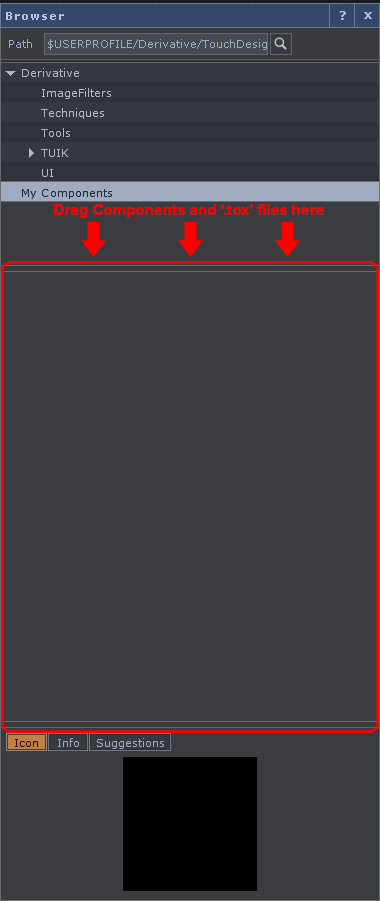
\includegraphics[width=6cm]{./img/2.6/palette-1.png}
\end{center}

\end{fullwidth}
%------------------------------------------------
\section{Search Dialog}

\begin{fullwidth}

The 'Search Dialog' is incredibly helpful as projects become more complicated, and riddled with Python scripts and nested Networks. The 'Search Dialog' can find a multitude of things in a multitude of places, and searches can be as broad, or specific, as needed. It is accessible in the 'Edit' menu at the top of  the screen, or by pressing 'F3' on the keyboard.

The 'Basic' search can not only find Operators, but can search through Python code. Frequently, Python is used to change Operator parameter values. Sometimes, in the thick of Python scripts, it is easy to lose track of specific lines of code. A quick search for the code below will return a list of every single line of code that involves changing parameters of the Operators with 'transform' in their name:

\begin{lstlisting}
op('transform').par
\end{lstlisting}

Sifting through the results is much easier than manually looking through Networks full of code. 

The 'Advanced' search can search by any combination of name, Operator type, comments, flags, and more. When returning to past projects, often it takes some time to relocate and reacclimatize to the inner workings of complex logic systems. This is when searching for operators by vague name and type can save a ton of time. For example, in an extremely nested system, somewhere in the depths of it might be a Movie In TOP that has the word 'movie' in its name. These little pieces of information about the Operator type, and partial name, can be used to create a fairly precise search. 

When a search has yielded results, each result can be clicked on to open the Network in a new floating pane. Here, the results can be can quickly previewed, and simple changes can be made within this pane, without affecting the current work area.

\end{fullwidth}
%------------------------------------------------
\section{Realtime Flag}

\begin{fullwidth}

\begin{center}
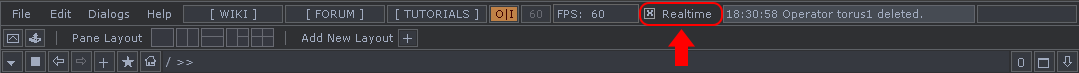
\includegraphics{./img/2.8/realtime-1.png}
\end{center}

The Realtime flag changes TouchDesigner's behaviour significantly. When it is active (it is active by default), TouchDesigner will always prioritize real-world time. In a simple example, if a movie file is 30 seconds long, no matter what happens, TouchDesigner will try to play it over the course of 30 seconds. If this means that frames need to be dropped, TouchDesigner will try to honour time. This is the mode used for most real-time installation and performance work. 

When the Realtime flag is off, TouchDesigner will prioritize frame rendering over real-world time. In the example mentioned above, if Realtime is off, TouchDesigner would take as long as it needed to process and render each frame, falling out of real-world time to display every frame. This mode is useful when exporting complex animations or 3D renderings. Imagine this mode to be similar to a real-time version of rendering out of Adobe After Effects. 

\end{fullwidth}
%------------------------------------------------
\section{Useful Shortcuts}

\begin{fullwidth}

Below is a bullet point list of some useful shortcuts:

\vspace{3mm}

\noindent When hovering over the Network:
\begin{itemize}
\item 'P' - Opens and closes the selected Operator's Parameter window
\item 'O' - Opens and closes a visual overview of the Network in the bottom-left corner of the pane
\item 'C' - Opens and closes the Colour Palette. This can add a coloured outline to the selected Operators for easier identification
\end{itemize}

\vspace{3mm}

\noindent With an Operator(s) selected:
\begin{itemize}
\item 'A' - Allows interaction with the Operator's viewer
\item 'B' - Bypass and un-bypass the selected Operator
\item 'H' - Performs the 'Home All' action on the Network, which is the equivalent to fitting all Operators of a Network onto the screen 
\item 'Shift + H' - Performs the 'Home Selected' action which fits all the selected Operators onto the screen 
\item 'R' - Toggles the Operator's Render Flag (if it has one)
\item 'D' - Toggles the Operator's Display Flag (if it has one)
\item 'Control + C' - Copy selected Operators
\item 'Control + V' - Paste copied Operators
\item 'Control + Shift + V' - Paste copied Operators at the mouse
\end{itemize}

\vspace{3mm}


\end{fullwidth}
%------------------------------------------------

%----------------------------------------------------------------------------------------
%	CHAPTER 3
%----------------------------------------------------------------------------------------

\cleardoublepage
\chapter{TOPs}
\label{ch:3}

%------------------------------------------------

\section{Introduction}

\begin{fullwidth}
Texture Operators, or TOPs, are a fundamental aspect of almost every project. They are the 2D texture Operators that handle everything from movie playback, 3D geometry rendering, compositing, hardware video inputs and outputs, and are used to process everything that will be output to a monitor, projector, or LED display.
\end{fullwidth}

%------------------------------------------------

\section{Movie In TOP}

\begin{fullwidth}
The Movie In TOP is one of the most used TOPs. It's function is to load assets into TouchDesigner. It is capable of loading many different types of assets, ranging from still images to a variety of movie codecs. Below is a small list of common file formats used with the Movie In TOP:

\begin{itemize}
\item .mov
\item .mp4
\item .avi
\item .tiff
\item .jpeg
\item .png
\end{itemize}

There are many more supported file formats, which are listed on the Derivative TouchDesigner 088 wiki under the 'File Types' page.

There are a few of great features built into the Movie In TOP that can significantly reduce the headaches involved with quickly ingesting and outputting assets with different frame-rates. The main feature is that the Movie In TOP's goal is to playback assets while staying true to it's time duration. For example, if the project is set to 60FPS and an asset is made at 30FPS and is 10 seconds long, it will play over the course of 10 seconds, regardless of FPS differences between the project and the asset. The opposite is true as well. If a 10 second asset created at 60 FPS is played in a 30FPS timeline, it will play over the course of 10 seconds. In both of these cases frames are either doubled or discarded to stay true to each asset's real-world time length. This makes interpolation of frames a good idea in some situations.

\end{fullwidth}

%------------------------------------------------

\section{Preloading Movies}

\begin{fullwidth}
When creating real-time applications, continuous dropped frames can greatly detract from presentation and impact. Diagnosing performance issues is something that will be discussed in a later chapter, but many preventative measures can be taken. Preloading and unloading Movie In TOPs is one of these preventative measures. The simple procedure of preloading and unloading movies is often overlooked by new users because the easiest methods involve scripting.

Open example 'Preloading.toe'. This example has a set of three buttons. The 'Preload' button uses the following Python function to preload the number of frames set in the 'Pre-Read frames' parameter in the 'Tune' parameters of the Operator 'moviein1':

\begin{lstlisting}
op('moviein1').preload()
\end{lstlisting}

The 'Play' button starts playback of the Movie In TOP. The 'Unload' button stops 'moviein1' playback, and then unloads the movie, freeing up whatever system resources were being used. This is done with the following Python script:

\begin{lstlisting}
op('play').click(0)

op('moviein1').unload()
\end{lstlisting}

It is best practice to preload movies before playing them, otherwise there is a high risk of dropping frames upon playback.

\end{fullwidth}

%------------------------------------------------

\section{Null TOPs and Select TOPs}

\begin{fullwidth}
In contrast to expensive TOPs, like the Blur TOP, some TOPs are 'free', and should be used generously! Two specific examples are Null TOPs and Select TOPs. These two Operators, although they don't alter any pixel, are incredibly helpful in creating more efficient workflows.

The difference between an illegible network, with wires overlapping and sprawled everywhere, and an easily followable Network are some properly placed Null TOPs and Select TOPs. Open examples 'Null\_1.toe' and 'Null\_2.toe'. The first file is a mish-mash of TOPs which are composited together. In this file, there is little regard for the layout of the Network, and the wires are overlapped by other Operators and other wires, making it difficult to trace any particular series of Operators. In 'Null\_2.toe' a column of Null TOPs are laid out to gather all the signals before they are composited. This column of Null TOPs can serve as a checkpoint, and even at quick glance, makes it much easier to follow series of operations.

The same case can be made for Select TOPs. When working with nested Networks, using the Out TOP and pulling connections between containers can lead to the same situation as above, where Networks become illegible rather quickly. The Select TOPs can quickly and neatly reference other TOPs. Open example 'Select\_1.toe'. This examples demonstrates how using In TOPs and Out TOPs can lead to extra clutter. This example is only replicating the movie 12 times! What would happen if there needed to be 100 of them? This is where the Select TOP comes in handy.

Open example 'Select\_2.toe'. This example exponentially increases the amount of replicated components while being simultaneously more legible. Even more interesting is the dynamic selection system created using the Select TOPs. This is much more efficient than the manual method from before, and allows a Python script in the Select TOP's 'Select' parameter to automatically reference the corresponding replicated TOPs from the Network above, based on the digits in their names. To take this concept one step further, a Select DAT is used to drive a Replicator COMP that creates a new Select TOP, and automatically wires it to the Composite TOP every time a new item is added with the first Replicator COMP. Don't worry if this example seems daunting, Replicators and Scripting will be covered in later examples. For now, the important thing to note is that by using Select TOPs and very simple scripting, this component is relatively future-proof and won't require much maintenance. When it comes time to  replicate more items, it's as easy as adding a row to a table.
\end{fullwidth}

%------------------------------------------------

\section{Codecs}

\begin{fullwidth}
Movie playback is a taxing process. It is wise to spend time experimenting with different codecs to see which one suits a project in terms of visual quality and performance.

Before diving into specific codecs, it is important to know the difference between a codec and a container. Codec has taken over as the general term for the file format of audio-video files, which is confusing for beginners, because many containers can hold multiple codecs. 

Codec stands for compressor-decompressor. The codec has two main tasks. The first it to compress video data for storage and transportation, and the second is to decompress the video data for playback. Because of these different tasks, each codec is made for a different purpose. Some prioritize compression for light weight, portable files, while others prioritize quality, for long-term preservation of content. Different projects will have different requirements. Sometimes, the goal is to play back a single piece of content at the highest quality possible, whereas other times, quality must be sacrificed to be able to playback multiple video files simultaneously. Finding the right codec for each project may require a few tests and some forethought, but it is time well spent. 

A container does exactly what its name implies. It holds the compressed video, audio, and all the metadata a movie player needs to properly decompress and playback the content. There are quite a few different containers, but they have much less of an impact on the overall programming workflow, compared to codecs. 

Things can get complicated when different combinations of containers and codecs are used. Imagine a file named 'test\_movie.mov'. In one example, this file could be an Animation codec compressed video file inside of a '.mov' QuickTime container. What's interesting, and what also confuses many beginners, is that in another example, this file could be an H.264 compressed video file inside of a QuickTime container. To add to confusion, the same H.264 file could also be inside of a '.mp4', or MPEG-4 Part 14, container. 

Confusion aside, some popular codec choices are currently the HAP family, H.264, Animation codec, and Cineform. Each codec has its own set of advantages and disadvantages. Below is a very quick point form list of some pros and cons to each:

\vspace{3mm}

\noindent \textbf{HAP family}

\vspace{3mm}

Pros
\begin{itemize}
\item Can playback extremely high resolutions and high frame rates
\item Very little CPU cost
\item HAP Q is visually lossless
\item Very little GPU cost
\end{itemize}

\vspace{3mm}

Cons
\begin{itemize}
\item Large file sizes
\item Difficult to batch encode files on Windows
\item Must use SSDs or a RAID0 of SSDs for file playback
\item Main bottleneck is hard drive read speeds
\end{itemize}

\vspace{6mm}

\noindent \textbf{H.264}

\vspace{3mm}

Pros
\begin{itemize}
\item Creates extremely light-weight/low file size videos
\item Best bang for buck when comparing quality to file size
\item Low disk usage
\end{itemize}

\vspace{3mm}

Cons
\begin{itemize}
\item Can't playback extremely high resolutions or high frame rate files because each file is limited to use a single CPU core for decoding
\item Can experience colour quantization if proper care is not taken in encoding
\item Bit rate is highly dependant on content
\item 4096 pixel size resolution in both length and width
\item Difficult to create alpha channels
\end{itemize}

\vspace{6mm}

\noindent \textbf{Animation Codec}

\vspace{3mm}

Pros
\begin{itemize}
\item 100\% quality is a lossless file
\item Prioritizes quality 
\item Has native support for Alpha channel 
\end{itemize}

\vspace{3mm}

Cons
\begin{itemize}
\item Large file sizes
\item Demanding on both hard drives and CPU
\item Bit rate fluctuates with amount of detail in video content
\end{itemize}

\vspace{6mm}

\noindent \textbf{Cineform} 

\vspace{3mm}

Pros
\begin{itemize}
\item Constant bit rate
\item High image quality
\item Native Alpha channel support
\end{itemize}

\vspace{3mm}

Cons
\begin{itemize}
\item Large file sizes
\item Must purchase encoding software from Cineform
\end{itemize}


\end{fullwidth}

%----------------------------------------------------------------------------------------
%	CHAPTER 4
%----------------------------------------------------------------------------------------

\cleardoublepage
\chapter{CHOPs}
\label{ch:4}

%------------------------------------------------

\section{Introduction}

\begin{fullwidth}
The Channel Operators, or CHOP, family of Operators handle all channel operations including motion data, audio inputs, key-frame animations, hardware inputs (from Microsoft Kinect, Leap Motion, Oculus Rift, pen tablets, keyboards, mice, etc), DMX, MIDI, and OSC. These are the Operators that handle inputs, processing, and outputs, of the data used to communicate with many types of audio-visual gear such as:

\begin{itemize}
\item Mixers
\item MIDI controllers
\item Synths
\item DMX lighting fixtures
\item Microsoft Kinect cameras
\item Computers running TouchDesigner
\item Loudspeakers
\item Other audio-video application like Max/MSP, Ableton Live, Resolume Arena
\end{itemize}

\end{fullwidth}

%------------------------------------------------

\section{Communication Methods}

\begin{fullwidth}
MIDI works with an extensive amount of existing software and hardware. Digital Audio Workstations, or DAWs, like Ableton Live, Avid Pro Tools, Propellerhead Reason, and more, all support MIDI input and output. It is a relatively fast, stable, and time-tested protocol. Audio performance controllers often comes equipped with MIDI over USB. These controllers include inputs hardware with controls such as: buttons, faders, piano keys, touch strips, jog wheels, drum pads, and potentiometers.

Programming environments such as Cycling 74 Max/MSP, PureData, Native Instruments Reaktor, and more, have support for OSC messaging. OSC messaging has the benefit of modern networking technology, higher resolutions than MIDI, channel naming, and many structural improvements. OSC messaging can be sent over UDP or TCP connections, making it incredibly easy to network, and transmit long distances in real-time. Currently, OSC is more commonly used as a communication method between softwares and computer systems.

DMX is a protocol used by lighting fixtures and controllers. Many DMX fixtures have various channels for dimmers, various settings, built-in chases, RGB channels, motor automation, and more. Many lighting controllers and desks use DMX protocol to communicate with fixtures and video-computer systems. With the many types of controllers and desks available, their manuals will be invaluable when creating projects with them in mind. In general, all of a fixtures channels need to be accounted for, even if aren't being actively used. There are many ways to optimize the workflow of sending and receiving DMX data, mostly concerning the management and organization of channels. These will be looked at in later examples.

Sync In CHOP and Sync Out CHOP are used to frame sync internal and external instances of TouchDesigner. They use the OSC protocol for their underlying communication. These two Operators work by communicating the state of each frame on every synced machine. Once all sync machines confirm that they have rendered the current frame, they simultaneously move to the next frame. This sequence of events is repeated for every frame and keeps the synced machines always on the same frame. 
\end{fullwidth}

%------------------------------------------------

\section{Audio Inputs and Outputs}

\begin{fullwidth}
Audio can be processed from a variety of sources, and can be processed in a variety of ways. TouchDesigner is capable of processing audio from audio files, movie files, external audio interfaces, internet audio streams, and can even synthesize audio from nothing. 

Most projects involving sound design and audio tracks will include dedicated audio files. TouchDesigner is capable of reading and playing many standard audio formats such as MP3, AIFF, and WAV, through the use of the Audio File In CHOP and the Audio Play CHOP. These files can be looped, cued, re-pitched, and trimmed, allowing for flexible uses of samples and audio files.

The Audio Movie CHOP can be used to playback audio from a movie file. Instead of reading audio by referencing a file, this CHOP references a Movie In TOP. This is useful because it keeps the audio in sync with the video playing back in the Movie In TOP, and comes with a parameter that can be used to offset the audio to better match the video.

There are many different external audio interfaces that can be used with TouchDesigner. It is best to refer to the Derivative TouchDesigner Wiki and Forum for a more comprehensive list of compatible devices. 

These devices provide analog and digital audio inputs and outputs. These can be inputs from musicians and instrumentalists, audio mixing consoles, professional video cameras, other computer systems, and much more. These devices can output audio to many of the above mentioned destinations, as well as to loud speaker systems. The CHOPs used to communicate with external interfaces are the Audio Device In CHOP and the Audio Device Out CHOP. Each respectively handles the inputs and outputs, to and from, a project. There is an Audio SDI CHOP which is used in conjunction with the nVidia Quadro SDI card, to receive audio from external SDI sources. 

There are two different audio drivers that can be accessed from within TouchDesigner. DirectSound has been available since previous versions of TouchDesigner, and has been developed as a part of DirectX. It is a mature driver, having been in development for many years, and provides relatively low latencies even under heavy use. 

ASIO is a new addition to TouchDesigner 088. It has been developed by Steinberg to improve on one of DirectX's main drawbacks, which is that DirectX feeds all audio through the Windows operating system. Bypassing the operating system, the ASIO driver is able to communicate directly with external audio hardware, thus creating lower latencies than what was previously possible with DirectSound.

Once inputs and outputs are setup in TouchDesigner, they can be routed much like any other data. 

\end{fullwidth}

%------------------------------------------------

\section{Sample Rates}

\begin{fullwidth}
Many applications never expose the granular functions and operations that are happening behind the scenes. Because of this, many people aren't used to processing audio in a mathematical fashion. Audio is, at its core, numerical data being processed incredibly fast. Knowing this lays the groundwork for how to work with audio in TouchDesigner. 

Open up example 'Sample\_rates\_1.toe'. This example creates a very basic feature common in many audio applications: muting. This is achieved by using a Math CHOP to multiply the audio stream by the output value of a Button COMP, which is either 0 or 1. Like any other mathematical equation, a value, in this case each sample of audio, multiplied by 0 will always be 0. Similarly, a value, or audio sample, multiplied by 1 will be returned unchanged. These two states produce on and off states for this audio example.  

Let's take this example a step further by allowing the button to fade the audio in and out. Open example 'Sample\_rates\_2.toe'. 

This example takes the previous example and adds two Operators. The first is the Filter CHOP which smoothens the input value. This creates a smooth ramp between the two states of the button. The second is a Resample CHOP. 

The sample rate of different Operators is something that is overlooked by many beginners, but is essential to having artifact-free audio. The Oscillator CHOP is being sampled 44,100 times a second, and the Filter CHOP is being sampled 60 times a second. This discrepancy means that there will not be a 1:1 ratio between the samples of audio and the samples of the ramp when they are multiplied. More accurately, there will be a 735:1 ratio between samples of audio and samples of the ramp. This means when the two values are multiplied, the audio will step up or down in volume every 735 samples. Examine the diagram below, where the dotted blue line is a 1:1 ratio, and the dotted red line represents a 735:1 ratio.

\begin{center}
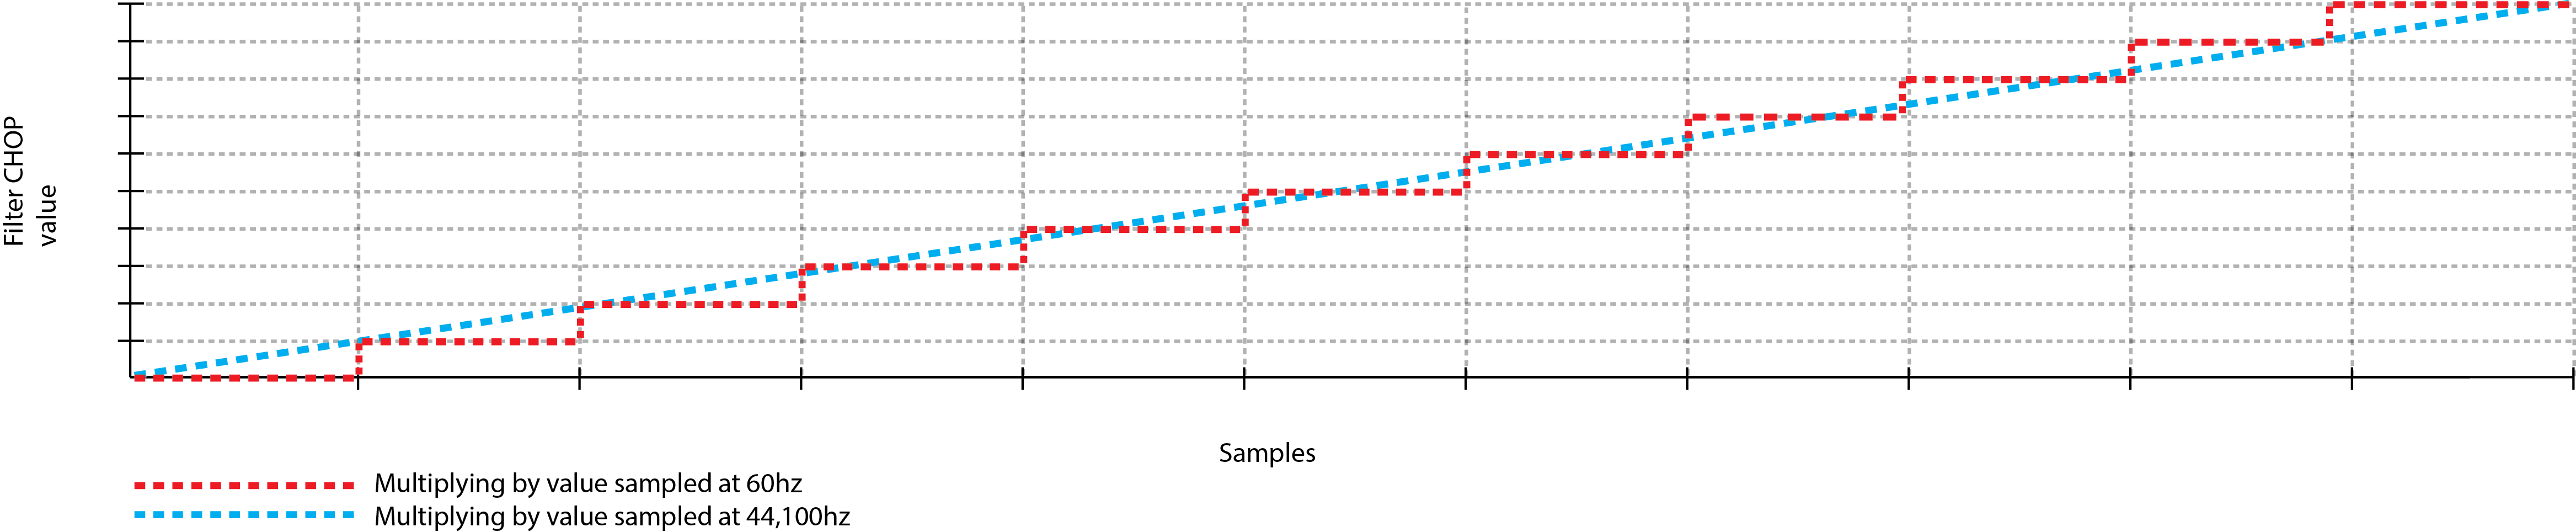
\includegraphics{./img/4.4/sample-rate.png}
\end{center}

Looking at the diagram above, there is a very distinct stepping that happens when the two channels that have different sample rates are multiplied. Many CHOPs use the project FPS as their default sample rate, causing the stepping to become exaggerated when the project is set to run at 30 FPS. Using the same example as above, the ratio of samples of audio and samples of the ramp would jump from 735:1 to 1470:1. This means in a 30 FPS project, there would only be an incremental volume change every 1470 samples! 

The above examples highlight the need to always be aware of the sample rates of CHOPs in a project, and to use the Resample CHOP when necessary. Many times, this situation will occur in regards to audio, but there are instances where control data might need to be input or output at a different sample rate. 

\end{fullwidth}

%------------------------------------------------
\section{Time Slicing}

\begin{fullwidth}

Time slicing is something that is unique to TouchDesigner, and can be a bit tricky to understand at first. 

A Time slice is the period between the last rendered frame and the current rendered frame. Think of Time slices as dynamic amounts of time. If a project is running at a consistent 60 FPS, then the time slices will be 1 frame in length. If a project is having trouble keeping up with real-time, and drops 10 frames, the corresponding time slice would be 10 frames in length.

Time slicing exists to smoothen out CHOP data in situations where frames are dropped. To think about it simply, Time slicing is when CHOPs start taking the size of Time slices into account when cooking. Think of this as a kind of adaptive cooking, meaning that as the time slices grow in length, the CHOPs will compensate for the amount of frames lost, and cook the amount of frames necessary to produce smoother outputs. This is in contrast to CHOPs that aren't time sliced, that will cook their value at the last cooked frame, then jump to the value at the next cooked frame, no matter how many frames are dropped inbetween. Only CHOPs can take advantage of Time slicing.

Using the example above, when the timeline is running consistently at 30 FPS, every time slice is 1 frame in length. If there are two ramps going from 0 to 1 over the course of one second (30 frames), both outputs would be smooth ramps. If, for some bizarre reason, only every tenth frame was cooked, there would be very different results. In the non-time sliced CHOP, the value would jump every time a frame is cooked, while the data between those cooked frames is lost. The Time sliced CHOP is aware that it is only being cooked every tenth frame, and will cook the frames inbetween to interpolate between the value of the last cooked frame, and the current cooked frame. This keeps the data smooth no matter what is going on. 

The diagram below illustrates the above example, where the dotted-blue line is a non-Time sliced CHOP, the dotted-red line is a Time sliced CHOP, and the vertical dotted-green lines represent a cooked frame: 

\begin{center}
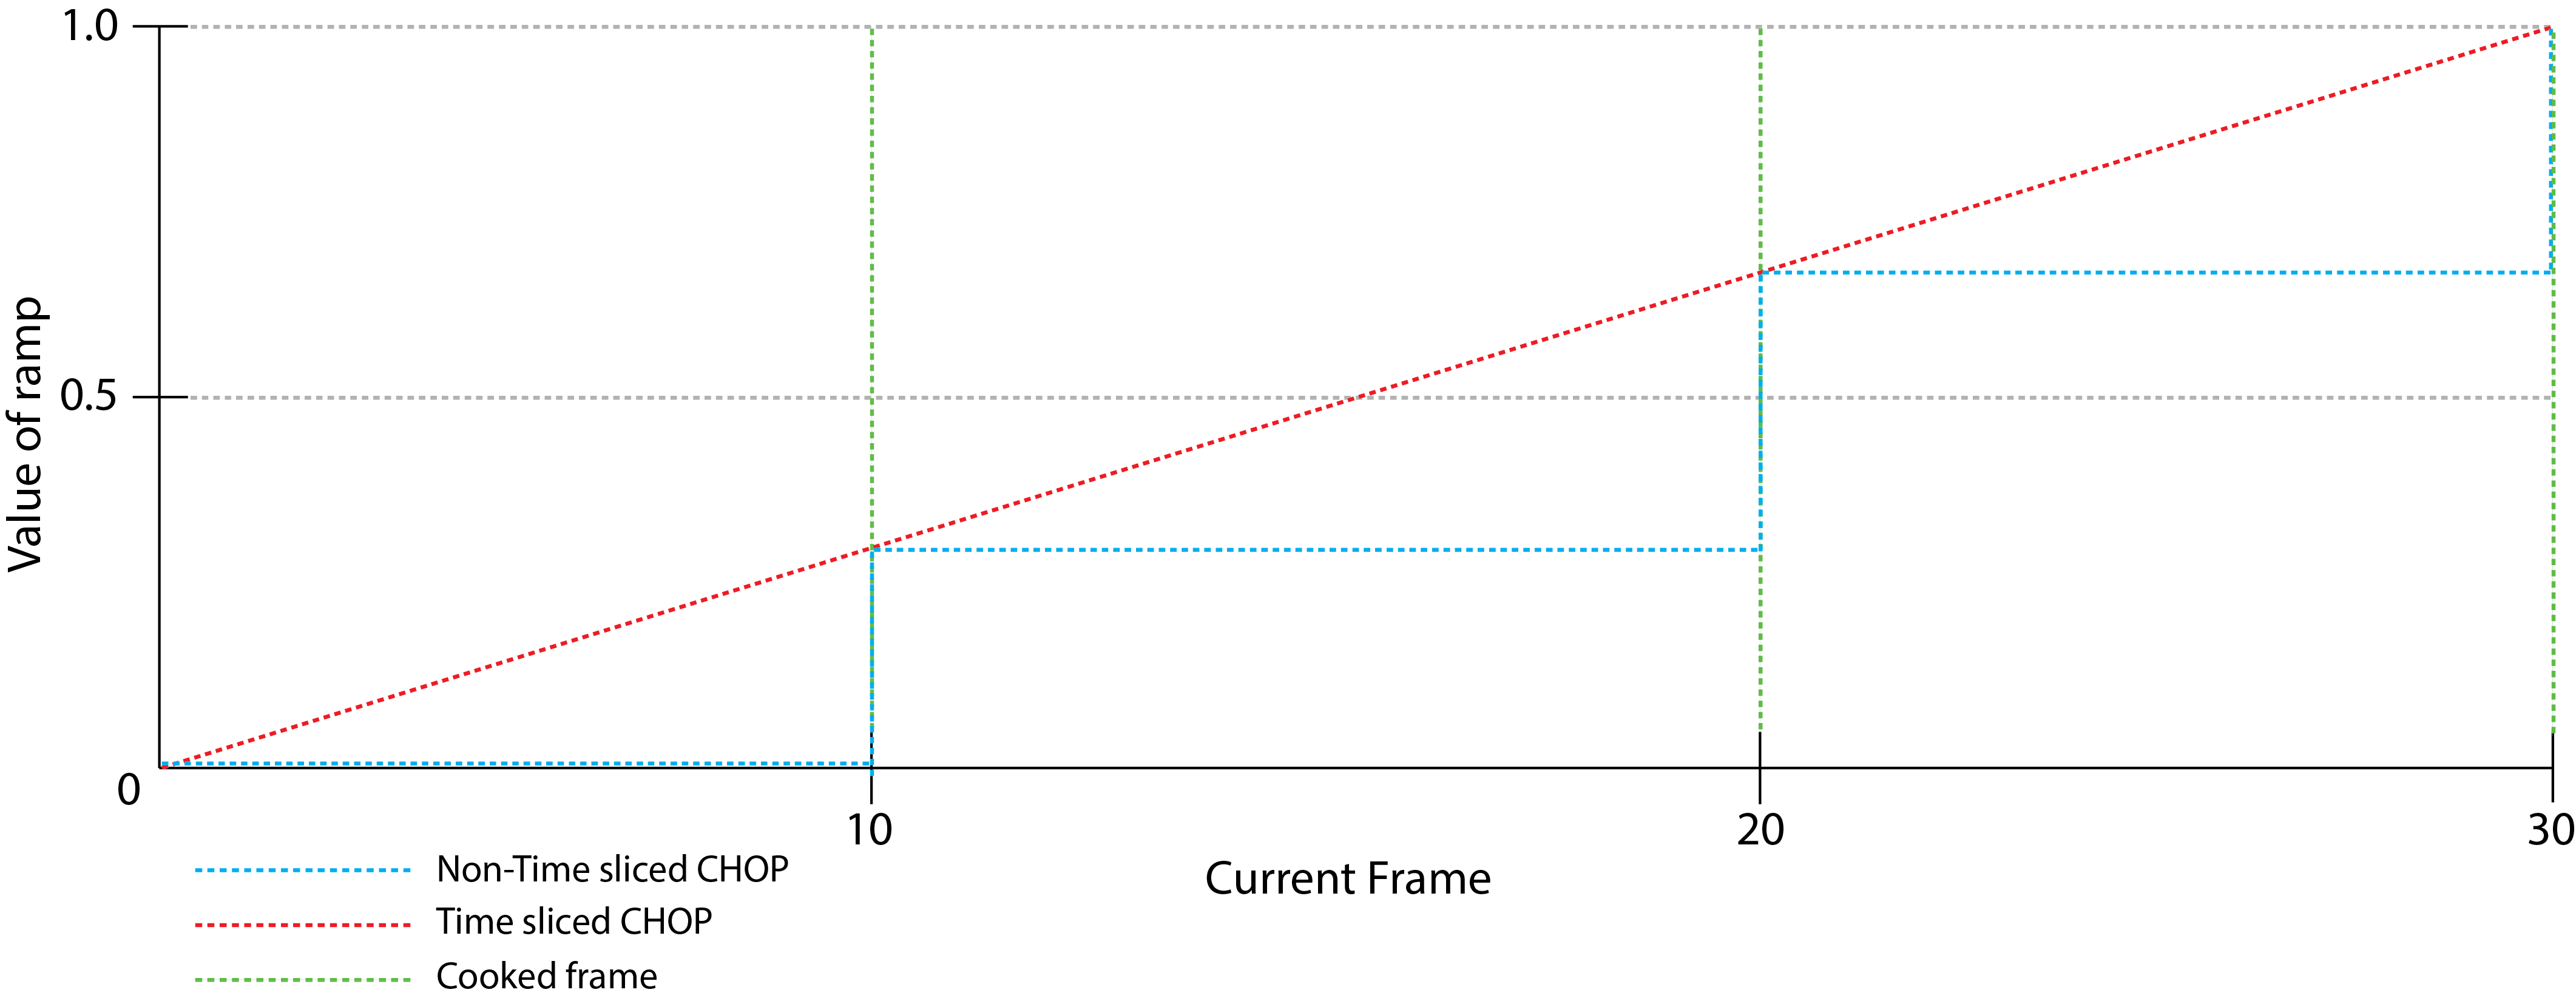
\includegraphics[width=14cm]{./img/4.4/Timeslice.png}
\end{center}

\end{fullwidth}


%----------------------------------------------------------------------------------------
%	CHAPTER 5
%----------------------------------------------------------------------------------------

\cleardoublepage
\chapter{DATs}
\label{ch:5}

%------------------------------------------------

\section{Introduction}

\begin{fullwidth}

Data Operators, or DATs, perform operations on data. They can edit, parse, create, send, and receive data in various forms. These forms of data can range from text strings, tables, Python scripts, XML, JSON, MIDI, Serial, OSC, and much more.

Logical systems rely heavily on the use of DATs and Python scripting. Being able to parse tables full of information and metadata, monitor other Operators and their states, perform complex tasks based on incoming messages from other systems, and more, make it possible to create rather complex systems in TouchDesigner. There will be a few simple logical systems in the examples portion of the book, as they are one of the things that makes TouchDesigner unique.

An interesting way of thinking about TouchDesigner 088 is as a modular Python programming environment. Imagine taking intricate, and long, Python programs and functions, and breaking them into light-weight, and modular pieces. Think of the Text DAT as these pieces. This setup is easy to learn from, easy to maintain, easy to expand upon, and even more importantly, easy to share and work on collaboratively.

\end{fullwidth}

%------------------------------------------------

\section{Communication Methods}

\begin{fullwidth}

There are quite a few DATs that are capable of providing inputs and outputs over the many standard communication protocols. TouchDesigner is able to communicate natively over MIDI, OSC, TCP, UDP, UDT, and Websocket, giving it the ability to speak to many different types of programs, web applications and services, show control hardware, other computer systems, and etc.

MIDI, OSC, and DMX protocols were explained in the CHOP chapter. DATs can communicate over the same protocols, and quite a few more.

TCP is the internet standard communication protocol. It is a connection oriented protocol, meaning there is a clear client-server relationship between the communicating parties, and a connection must be established (usually behind the scenes) before any data is transmitted. This relationship allows TCP connections to be reliable, in that the communicating parties can provide acknowledgment of all data sent and received, meaning no data ever gets lost. TCP is an ordered delivery stream, meaning data sent in a specific order, will be received in that same order.

UDP, on the contrary, is a connection-less protocol, in that no explicit connection is established prior to data transmission. This creates a level of unreliability in areas such as delivery acknowledgments, dropped packets, and order of messages. If none of these are crucial to a project, there are some performance gains in systems where dropped packets are less of an issue than delayed packets. 

UDT is one of the newer communication protocols. It is essentially the better parts of UDP and TCP combined. It is built on the UDP protocol, but is connection-based, and reliable. This means that is has the same acknowledgments and data ordering that a TCP connection would have, but over the faster UDP protocol.

A benefit of connection-less protocols is that they support a feature called 'Multicast messaging'. This means that regardless of how many computers are connected, each message is only sent over the network once. When sending the same message to many computers, this removes the overhead of sending the same message to each individual computer. This is the opposite of 'Unicast messaging', in which each connected computer receives an individual message, even if the message being sent to every machine is the same.

Websocket is the go-to communication method when working with web browsers and real-time web application. It has been designed from the ground up to be used as an interface between web browsers and servers, and the protocol has simplified some key functionality in regards to bi-directional web communication. 


\end{fullwidth}

%----------------------------------------------------------------------------------------
%	CHAPTER 6
%----------------------------------------------------------------------------------------

\cleardoublepage
\chapter{SOPs}
\label{ch:6}

%------------------------------------------------

\section{Introduction}

\begin{fullwidth}

The Surface Operators, or SOPs, family of Operators are used for any and all 3D operations. This includes working with simple 3D geometry, particle systems, architectural models, 3D characters, and more. SOPs are the oft ignored operators by many beginners because of their steep learning curve, but rest assured that a firm knowledge over the SOP family of operators will open up many incredibly interesting opportunities, project wise, as well as offer many extremely efficient ways of solving problems.

Many projects involving projection mapping, real-time 3D motion capture, architectural LED facade installations, and layered video players, would either be impossible or extremely difficult without the SOP family of operators.

TouchDesigner 088 currently supports the following 3D file types:

\begin{itemize}
\item .fbx
\item .obj
\item .3ds
\item .dxf
\item .dae
\end{itemize}

Keeping Operators from cooking needlessly is essential to smooth performance, which will be discussed further in the 'Optimization' section of the book. This is even more important when it comes to SOPs. Always try to apply transform animation data to a Geometry COMP instead directly of to a SOP. This is because SOP transformations happen on the CPU, and the transformation must be performed for every vertex that is present in the geometry. Component level transformations are applied to the 3D geometry, or object, as a whole, and are performed on the GPU as a single operation. A single operation performed on the GPU is much preferred when compared to what could amount hundreds or thousands of operations performed on the CPU. 

The number of total points, primitives, vertices, and meshes will vary depending on what kind of model is being processed, but the basic principle is that the more polygons/vertices in a model, the more processing power and GPU RAM are needed to process operations. There are tools inside of TouchDesigner to reduce polygon counts in complex models, but optimizing geometry in dedicated modelling suites can provide more flexibility.

\end{fullwidth}


%------------------------------------------------

\section{Rendering}

\begin{fullwidth}

One thing many beginners struggle with is the process of quickly and effectively transitioning from a 3D workflow to a 2D workflow. The Internet is full of 3D workflow tutorials that can explain many of the finer points of 3D rendering, but for this chapter, the goal is to get from point A, a simple 3D object, to Point B, a Render TOP.

There are three parts to a 3D scene:

\begin{enumerate}
\item 3D geometry (and materials)
\item Camera
\item Lighting
\end{enumerate}

Open example 'Rendering\_1.toe'. Taking a quick look at it, there are three basic things needed to render the scene, Camera, Light, and 3D geometry, which are all referenced by a Render TOP. Let's break down each aspect of the render setup, and then look at how it all fits together.

The appropriate place to begin is the 3D geometry. This is the essence of it all. The 3D model can be anything from simple polygons, animated 3D characters, architectural models, etc. Whether importing or procedurally building models, all of the operations are done with SOPs, and these SOPs end up in a Geometry Component. A key idea to grasp is that in TouchDesigner, SOPs themselves are never directly rendered. Instead, Geometry Components, or Geometry COMPs, are rendered, that hold SOPs that are flagged for rendering. This is a crucial idea to understand. Two scenarios demonstrate this.

Open example 'Rendering\_2.toe'. In this project, there is a single geometry that is sent into 4 different Geometry COMPs, each of which is rendered with different transform values. For the sake of example, this project uses a Box SOP, but in this could apply to more complex models. Performing operations on a complex character, and having a few iterations of it, could max out a systems headroom. Going back to the idea that SOPs aren't directly rendered, it becomes logical to load the model once, from which a few iterations can be housed and rendered from Geometry COMPs.

Open example 'Rendering\_3.toe'. This is very different than the previous example, in that there is a single Geometry COMP with 3 different models that are being rendered. Keeping in mind that Geometry COMPs are rendered, it becomes logical to group these models into a single Geometry COMP, that is being rendered. The difference may seem arbitrary, but as projects become more complex, saving resources becomes paramount.

Till now, the various geometry haven't had any materials. Materials are what make 3D scenes interesting. The difference between a cement building-block and a 3D box is a material. Textures can be applied at two levels: the SOP level, and the Component level. The first is through the use of the Material SOP, and the second is by referencing the material in the 'Render' tab of a Geometry COMP. In the example 'Rendering\_4.toe', both materials look the same, but each use a different method of texturing.

Now that materials are added to the mix, let's quickly discuss UV maps. Open example 'Rendering\_5.toe'. This is the same example as above, but the same texture looks completely different. This is because the co-ordinates of the UV map have been changed.

The second aspect of a 3D scene is light. Just as in real life, 3D scenes require lighting. Open example 'Rendering\_6.toe'. This example has a simple box being rendered, but nothing is visible in the Render TOP. This is because the light's dimness has been purposefully set the to 0, to demonstrate how important lighting is, and how it is often overlooked.

The next few example projects are the same scene with different lights. In each consecutive project, the Light COMP has been transformed to light the Box SOP from a different angle. These are example projects 'Rendering\_7.toe', 'Rendering\_8.toe', and 'Rendering\_9.toe'.

The last aspect to rendering a 3D scene is the camera. The camera is the eye and perspective. What the camera sees is what gets rendered. Open example 'Rendering\_10.toe'. All the movement in the scene stems from the animated camera movements. Often times, a camera is placed in a scene and never thought about again. This can lead to boring 3D scenes that feel very static and lifeless. Don't be afraid to think like a cinematographer, and experiment with camera positions, focal lengths, and animated camera movement.

There are two main types of cameras: perspective cameras and orthographic cameras.

\begin{center}
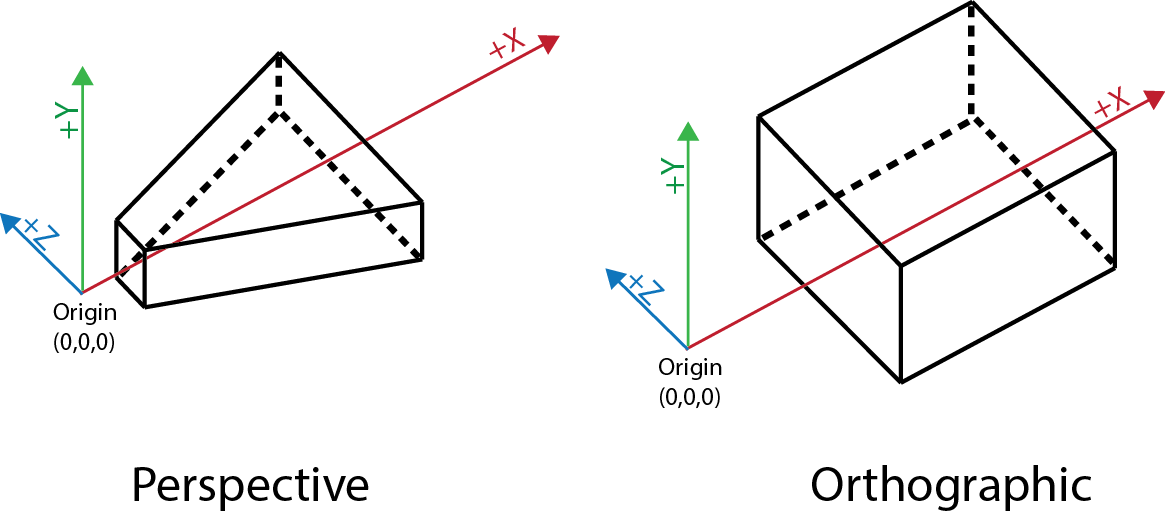
\includegraphics{./img/6.2/rendering-1.png}

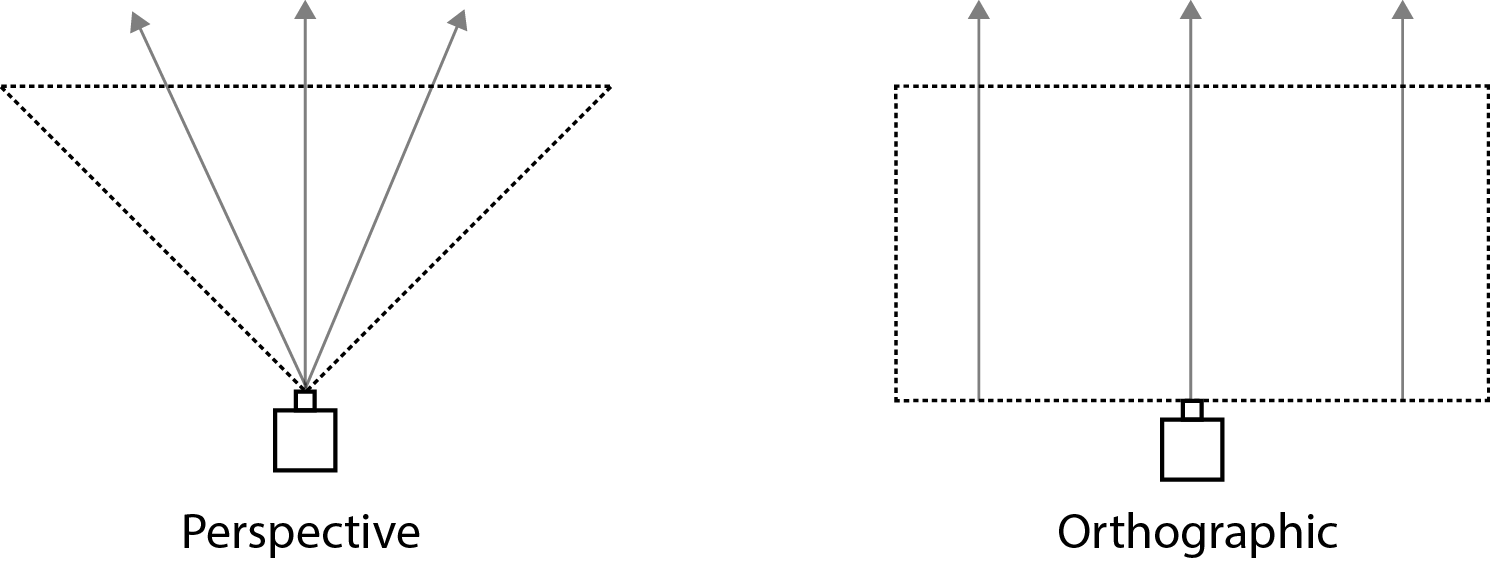
\includegraphics{./img/6.2/rendering-2.png}
\end{center}

Perspective cameras need very little explanation, as they work similarly to the human eye. Perspective cameras have a perspective point, and a view frustum that are used to determine what the camera sees and how that is rendered. With a perspective camera, imagine all light in the 3D scene funnelling towards the perspective point. Perspective correction, or 'foreshortening', is applied on all objects in the scene, meaning that objects farther away from the camera appear smaller. This camera ends up being used most often as it functions like human eyes. An example of this type of camera can be found in example file 'Camera\_1.toe'.

This example highlights perspective correction. There are two cubes, both the same size. The cube placed farther in the scene appears smaller, just as it would in real life. This is the simplest example of how a perspective camera functions.

Orthographic cameras, on the other hand, are very different. Those familiar with computer-aided design (CAD) software, may have encountered orthographic cameras before. The key principle behind an orthographic camera is that there is no single point of perspective. All of the light in the imaginary 3D scene would not filter into a single point, as in a perspective camera. Objects are not distorted by their Z position in space, meaning that no matter how far away from the camera an object is, it will appear no bigger or smaller than the other objects in the scene. 

Open example 'Camera\_2.toe'. This example is exactly the same as 'Camera\_1.toe', but there is a big difference in what is being rendered. In this example, the two cubes appear to be side by side, regardless of positioning in Z space. This can be a hard concept to understand the first time it is presented. Two ways of thinking about it are as follows:

\begin{description}
\item[First] The concept of a 3D world that gets squashed onto a single plane before it gets rendered. Imagine the original Super Mario video game actually being a 3D scene that was rendered using an orthographic camera. No matter where bad guys and platforms are on the screen, whether at the edge or in the middle, they are always the same size and shape, and have no perspective correction applied.
\item[Second] Think about the blueprint of a building in a CAD program. It is a representation of a 3D object on a 2D plane. No matter where the blueprint is perceived from on screen, 1 unit of measurement on the edge of the screen is exactly the same length as 1 unit of measurement in the middle of the screen. Any change in the camera positioning doesn't distort what is being rendered.
\end{description}

None of this is to say that Z-depth is irrelevant when using an orthographic camera. Z depth becomes imperative when layering different pieces of geometry in a scene. 

The camera is equally important for projection mapping projects. Projection mapping will be explored in later examples, but for now, the key is to understand another of the Camera's roles. In projection mapping, the primary goal is to turn real-world objects into 3D display surfaces. To achieve this, a 3D model of the object is imported into TouchDesigner and textured using a variety of sources. This textured object then needs to be rendered. Camera COMPs come into play to simulate real-world projectors. Gathering as much information about the characteristics of a projector and it's lens, the Camera COMP can accurately replicate the point of view of the projector inside of TouchDesigner. These points of view are then rendered, output, calibrated, and lined up to the real-world object. This is the basis of projection mapping. 


\end{fullwidth}

%----------------------------------------------------------------------------------------
%	CHAPTER 7
%----------------------------------------------------------------------------------------

\cleardoublepage
\chapter{COMPs}
\label{ch:7}

%------------------------------------------------

\section{Introduction}

\begin{fullwidth}
There are 3 types of Component Operators, or COMPs, and each have different uses:

\begin{description}
\item[Object] components create, light, and view 3D scenes
\item[Panel] components create UI components such as buttons, sliders, and window panes
\item[Other] components include components that create keyframe animations, replicate other Operators, and create output windows
\end{description}

Component Operators are generally used in conjunction with other Operators. The 'Object' components are used in various combinations to create and render SOPs and 3D scenes. The 'Panel' components are used to create UIs and various containers to create output rasters. The 'Other' components are used for various tasks, such as keyframe animations, dynamic Operator replication, opening windows on various displays, etc.

An interesting fact to put things in perspective is that a large amount of TouchDesigner is made from components inside of TouchDesigner. Understanding this really helps in grasping the granularity of TouchDesigner, and how to approach working on various projects. For example, all Panel components are made of other Operators. Create a Button COMP, and inside it's Network, it's background is made of a Text TOP, and its on/off values are being generated by a Panel CHOP. Similarly, all of TouchDesigner's UI is made and stored in the 'ui' container in the root of all projects. Even the menus and dialogs, like the MIDI Mapper Dialog and the Variables Dialog, are created using other TouchDesigner components.

\end{fullwidth}

%------------------------------------------------

\section{Window COMP}

\begin{fullwidth}
The Window COMP is used in almost every project to display the contents of an Operator in a new window. Whether using the Window COMP to create a full-screen output, or to create more of a traditional windowed application, there are a number of options that will need modifying. Because of the unique nature of every project, there are no 'best settings' to consistently rely on. Spend some time and go over the parameters on the Wiki, and experiment to find works best in each and every new situation.

Open example 'Window.toe'. This example demonstrates a very helpful practice, as well as some simple Window COMP functionality. It is best practice to use a Container COMP as the source of the Window COMP's output. This is because the texture in a TOP can be dragged around the screen, even in Perform Mode. If this happens, the texture will remain shifted until the project is reloaded, or until the texture is moved back to it's original position. The same texture shifting doesn't occur to Container COMPs. The texture inside of a Container COMP cannot be dragged around by default, meaning the texture will always be consistent.

The other functionality in this example is rather simple. The first is a button, whose Null CHOP is being referenced in the 'Open in Separate Window' parameter of the Window COMP. This allows easy access to the opening of the window. The next is a button that dynamically checks how many monitors are connected, by getting a row count from the recently implemented Monitors DAT. Using that value to cycle a Count CHOP, open the window with the first button, then use the second button to cycle through which monitor this window is assigned to.
\end{fullwidth}

%------------------------------------------------

\section{User Interface Components}

\begin{fullwidth}
Component Operators are incredibly important as they create user interfaces in TouchDesigner. Specifically, the Panel Components are what provide this functionality. Many user interfaces will be created in later examples, so only a few basic examples will be examined in this section.

Three of the most useful Panel COMPs are:

\begin{itemize}
\item the Slider COMP
\item the Button COMP
\item Container COMP
\end{itemize}

The first two function with the same capabilities as sliders and buttons in other applications, but can be modified to suit different requirements. Buttons can be programmed as toggles, radios, or momentary buttons. Sliders can function as single axis sliders, or as full XY pads.

Container COMPs, on the other hand, don't have a function other than acting as a container for other UI elements.

Open example 'UI.toe'. In this example, there is a simple UI. From the bottom of the Network upwards, there are the 2 Button COMPs and the 5 Slider COMPs. These are the components that are actually creating the UI's functionality. The parent of these elements, is used to group and arrange the buttons and sliders separately. Notice that if the viewers for 'container1' or 'container2' are activated, the UI elements are usable, but neither 'container1' or 'container2' have any outputs or Operators in their Networks. Similarly, the results are the same when 'container1' and 'container2' are combined inside of 'container3'. This is because Container COMPs have the ability to display their children in their viewers. Container COMPs facilitate the creation of complex interfaces using a combination of smaller pieces.


\end{fullwidth}


%----------------------------------------------------------------------------------------
%	CHAPTER 8
%----------------------------------------------------------------------------------------

\cleardoublepage
\chapter{MATs}
\label{ch:8}
 
%------------------------------------------------

\section{Introduction}

\begin{fullwidth}
Material Operators, or MATs, are used for materials and shaders for 3D geometry.

A deep knowledge of computer graphics and rendering helps a great deal when working with materials and shaders. Without this knowledge, most users will be restricted to the basic settings of the Phong MAT and Point Sprite MAT.

Texturing and UV mapping geometry are involved processes, and the best results are often achieved inside dedicated modelling packages. The textured models can then be imported, and worked with, in TouchDesigner. 

Many tools exist for modifying textures, such as the Texture SOP, but complex processes might be easier to achieve in a software package created for that specific purpose.

\end{fullwidth}

%------------------------------------------------

\section{Phong, GLSL, and Point Sprite Materials}

\begin{fullwidth}

The three most used MATs are:

\begin{itemize}
\item the Phong MAT
\item the GLSL MAT
\item the Point Sprite MAT
\end{itemize}

The general uses of these three MATs will quickly be covered in this section. These are three very different Operators, and cover many shading and material needs.

The Phong MAT is the most common material Operator. It is responsible for applying texture to 3D geometry. There are a variety of maps that can be applied, such as Color, Bump, Specular, Diffuse, and more. The Phong MAT can mix and match Ambient, Diffuse, Specular, Emit, and Constant lighting. Open example 'Phong.toe'. In this project there are two very simple examples of the Phong MAT. The first uses the texture's alpha to create a transparent box. The second sets the Emit Light of 1,1,1 to fully illuminate the object regardless of the lighting condition. There will be many examples of the Phong MAT when it is put to use the examples section.

The GLSL MAT is used to create custom materials using the OpenGL Shading Language (GLSL for short). GLSL is a fantastic programming language that can create extremely complex textures that run extremely quickly. It achieves this by giving the programmer quite a bit of control over the graphics pipeline, without exposing them to assembly languages. There can be a slight learning curve when first starting, but there are tons of examples of GLSL shaders on the Internet, as well as quite a number of great examples in the 'Shared Component' area of the TouchDesigner Forum.

The Point Sprite MAT is used to assign sprites to the points of a particle system. The name is self explanatory, in that a 2D image (a sprite) is placed at every single point in 3D space. The sprites are always facing the camera, and are scaled according to their Z depth. The example 'Point\_Sprite.toe' demonstrates this. To create a similar TouchDesigner network without point sprites, not only would there be a pretty disorganized Network, of who knows how many Transform TOPs and Composite TOPs, but they would all be using much more resources. By using a particle system and point sprites, the Network is easy to read, and doesn't require a lot of system resources.
\end{fullwidth}

%------------------------------------------------

\section{UV Maps}

\begin{fullwidth}

UV mapping is an essential to working with complex 3D geometry. As with certain other aspects of 3D modelling, it is easier to create and work with UV maps in a dedicated modelling program.

UV mapping is what allows designers and artists to create interesting motion and still graphic textures for 3D geometry. It bridges the 2D world that motion and still graphics are created in with the 3D world of the geometry. 

UV mapping is a three-step process. The first step is the unwrapping of the 3D object into a 2D plane. This unwrapped texture is called a UV map. It is referred to as a map, because much like any other type of map, it takes a 3D object and accurately, and proportionally, creates a 2D reference. This is the same as street maps or world maps, that take the 3D universe and represent them on a 2D plane.

Texturing is the the second step. The 2D UV map is used by artists and designers in their compositing softwares to create textures, whether still or moving. The benefit of the UV map is that the textures can be applied to the geometry with a high degree of precision.

The third step is the application of the texture onto the 3D geometry. This varies depending on the software used.

The combination of these three steps are referred to as UV mapping.

The third step is a relatively common operation in TouchDesigner. As long as the 3D geometry is exported correctly from its modelling software, it will include co-ordinates indicating to other applications where the UV maps should be applied. In these situations the texture is loaded in a Movie In TOP and applied using a Phong MAT to the geometry. If any changes need to be made to how the UV map is applied, the Texture SOP can be used. 

Below is an example of a simple 3D box, and it's UV map:

\begin{center}
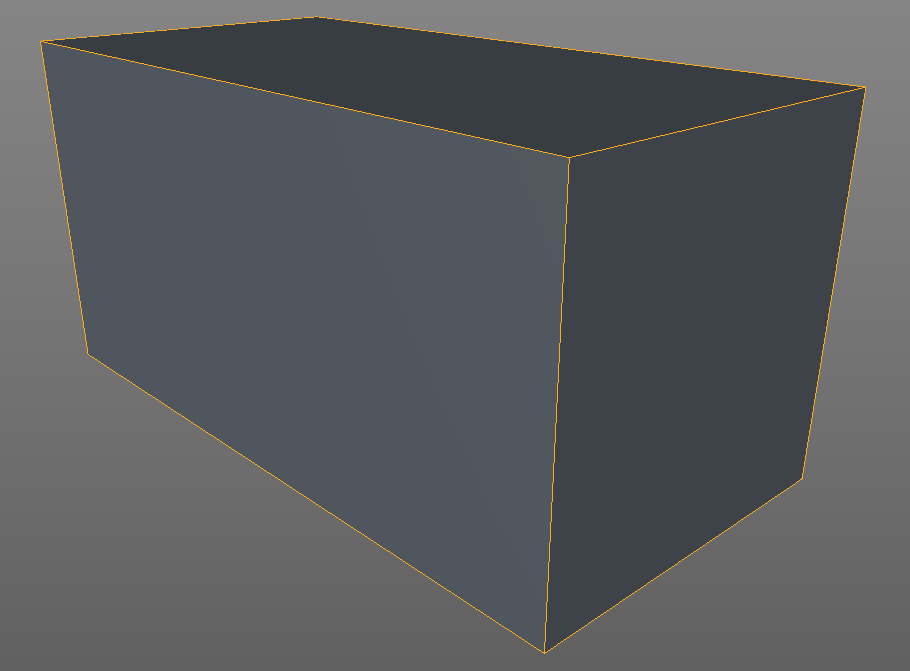
\includegraphics[width=15cm]{./img/8.3/3D-geo.png}

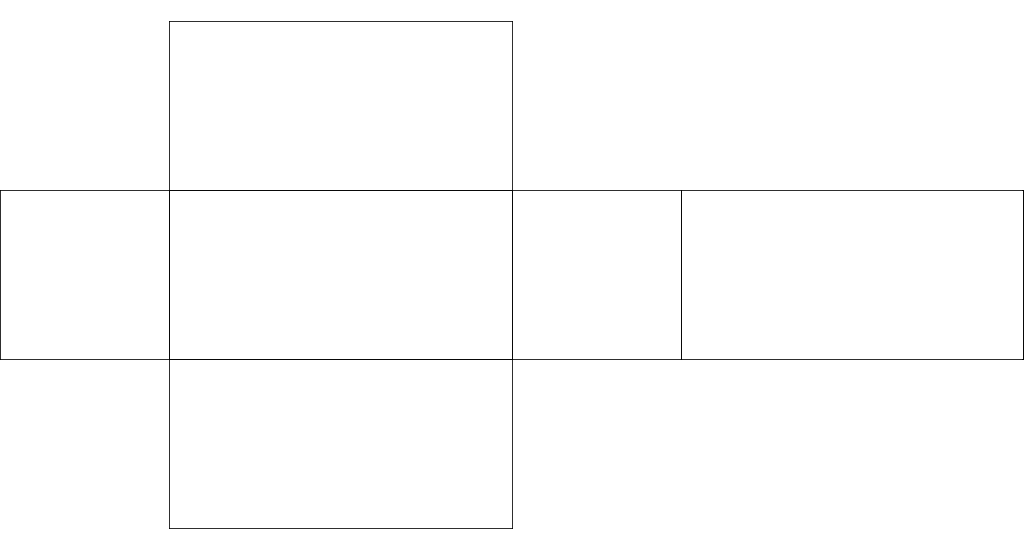
\includegraphics[width=15cm]{./img/8.3/Geo-map.png}
\end{center}

\end{fullwidth}


%----------------------------------------------------------------------------------------
%	CHAPTER 9
%----------------------------------------------------------------------------------------

\cleardoublepage
\chapter{Python}
\label{ch:9}

%------------------------------------------------

\section{Introduction}

\begin{fullwidth}
Python scripting is one of the most powerful features of TouchDesigner 088. It is capable of doing incredibly complex operations, like iterating through large data sets, natively communicating with a myriad web APIs, controlling and changing the parameters of other Operators in extremely rapid succession, and much more.

It is important to note that, as of writing, TouchDesigner 088 uses Python 3.3.1. Python 3 differs from Python 2.7 in a number of ways, but most issues can be resolved with a quick Google search. Most questions have probably already been asked, and the solution could be as simple as a set of parentheses.

For example, in Python 2.7, the Print function could be used without parentheses, where in Python 3, this will raise an error. Below is an example of how many Python 2.7 courses use the Print function:

\begin{lstlisting}
print 'text'
\end{lstlisting}

This is in contrast to how the Print function is used in Python 3, where the parentheses are required:

\begin{lstlisting}
print ('text')
\end{lstlisting}

An incredible feature of Python, aside from it's readability, is that there are many external libraries, many of which can natively connect to most of the webs most active spaces, like Facebook, Twitter, Instagram, Foursquare, etc. These kind of native integrations unlock a world of real-time data driven projects, as well as incredible real-time data sets for visualizations and client presentations.

There will be quite a bit of Python scripting in later examples, and although it is not mandatory to do so, it is highly recommended that some time be spent learning Python through introductory tutorials. There are many fantastic resources for learning Python, some of them gamified, and most of them often quite easy to pick up and put down. Often times, 10-15 minutes a day of tutorials, over the course of a few weeks, can provide a strong fundamental knowledge of Python, and more than enough knowledge to do quite a bit of scripting in TouchDesigner.
\end{fullwidth}


%------------------------------------------------

\section{Textport}

\begin{fullwidth}
The Textport has a few important roles in regards to scripting inside of TouchDesigner. There are two ways to open the Textport. The first is by using key command 'Alt + T'. The second is by selecting 'Textport' from 'Dialogs' in the menu bar at the top of the TouchDesigner window.

The first is that it can be used similarly to the IDLE shell that comes with Python installations. For example, open the Textport, type the following, and hit 'Enter' on the keyboard:

\begin{lstlisting}
print(2+2+2+2)
\end{lstlisting}

Running this in Python would print the result of the equation, which is 8. After hitting 'Enter' in the Textport, the result of the equation is displayed. This is because the Textport works as a Python interpreter. Type Python code into the Textport, it will be processed, and the results will be returned. 

It can similarly do the same for tscript, the scripting language that was used in TouchDesigner 077. Notice that when the Textport is opened, the first thing printed is: 

\begin{lstlisting}
python >> 
\end{lstlisting}

This is because in TouchDesigner 088, the Textport interpreter is set to interpret Python by default. To work with tscript in the Textport, the mode of the Textport needs to be changed from Python to tscript. This is done by clicking on the Python logo in the top left corner of the Textport. Once clicked, it will change to the letter 'T' and the next line of the Textport will be:

\begin{lstlisting}
tscript -> 
\end{lstlisting}

This means the Textport is now in tscript mode. To confirm this, type the following tscript code into the Textport:

\begin{lstlisting}
echo Hello!
\end{lstlisting}

Similar to the Python Print function, the above tscript code will print 'Hello!'' to the Textport.

Another great use of the Textport is as a Python debugger. Open example 'Textport\_1.toe'.

This is a very simple example that highlights how beneficial the Textport becomes when using Python scripts. Open the Textport, and then click on the 'Good Python' button in the middle of the Network. This will run a script that prints to the Textport:

\begin{lstlisting}
this will not error
\end{lstlisting}

Now click on the 'Bad Python' button. The Textport will display something very different.

\begin{lstlisting}
File "/project1/chopexec1", line 11
	Print(this will error)
			     ^
SyntaxError: Invalid syntax
\end{lstlisting}

This is a Python error, occurring because some of the code being interpreted is invalid. Learning to read these errors can greatly speed up debugging large Python scripts. Let's examine the different portions of this error.

The first line indicates exactly where the error is in the Network, and which line of the script the Python interpreter believes is invalid:

\begin{lstlisting}
File "/project1/chopexec1", line 11
\end{lstlisting}

In this example, the Operator with the error is 'chopexec1' inside of the component 'project1'. The Python stops interpreting the script at line 11.

Below that, the Textport prints the line with the error:

\begin{lstlisting}
Print(this will error)
\end{lstlisting}

More often that not, spelling mistakes and slip-ups can easily be caught by these two lines. In this case, it is clear that the string being printed is not enclosed in quotation marks. Knowing where the error is, and more specifically what the line the error is occurring on, means this would result in the problem being quickly solved. For the sake of this example look at the last line of the error:

\begin{lstlisting}
SyntaxError: Invalid syntax
\end{lstlisting}

The last line of the error is the type of error Python is encountering. More detailed information on the different types of errors can be found by looking through the official Python 3.3 documentation, under the 'Errors and Exceptions' section. The 'SyntaxErrror' is a very common error, and is caused by the Python interpreter encountering code that isn't valid Python syntax. As mentioned, the above line of code is the missing the quotation marks around the string being printed.

Printing to the Textport is an excellent way to take some of the mystery out of scripting. When scripting in larger and larger projects, there are often scripts in every Network, and quite often, many of them are performing backend tasks, such as preloading and unloading movies, that have results that are difficult to view. More often than not, scripts are running in parallel in different Networks, and it becomes incredibly difficult to tell if the timing of scripts are correct, or if actions are happening in the wrong order.

By having simple Print functions spread throughout scripts, it is not only easy to see when scripts are running, but myriad pieces of information can be printed as well. Some of these pieces of information can be as simple as the path to the script that is being run, or as detailed as what values and variables are being worked with and changed.

Open example 'Textport\_2.toe'. In this example, there are two sequences of scripts that run one after another, with a certain amount of pause between them. Click the 'Visual Sequence' button. This sequence has buttons that are clicked into the On position as each script is run. This is solely to make it easier to see the progress of this sequence. How would this progress be monitored from another Network?

Open the Textport and click the 'Textport Sequence' button. Contrary to the first sequence, this sequence prints a message to the Textport as each script is run. There may not be buttons visually changing states in the Network, but a number of new abilities are gained. The first is the ability to monitor these scripts from anywhere in the project. The second is that it is possible to compare the timing of these sequences to any other scripts that are running elsewhere in the project. The third, and possibly the most valuable, is the ability to pause the project and have a written history of the most recent sequence of events.

This history becomes absolutely invaluable when debugging complex logic systems. In a project with 30 Networks and 300 independent scripts, when a series of actions fail without raising any Python errors, without an ordered log of events, it would be impossible to trace bugs. As a script becomes longer and more complex, it is easy to create more of these pseudo-checkpoints throughout the script, such as 'running X section of Y script'.

\end{fullwidth}

%------------------------------------------------

\section{Common Practices}

\begin{fullwidth}

There are some common practices that should be upheld when working with Python. Something that is interesting about the Python language is that it is built around the idea of readability and simplicity. Python has an easter egg built inside of it, which can be accessed by entering the following code into a Python interpreter or the Textport:

\begin{lstlisting}
import this
\end{lstlisting}

Python returns a poem named 'The Zen of Python' by Tim Peters. Below is that text:

\begin{lstlisting}
The Zen of Python, by Tim Peters

Beautiful is better than ugly.
Explicit is better than implicit.
Simple is better than complex.
Complex is better than complicated.
Flat is better than nested.
Sparse is better than dense.
Readability counts.
Special cases aren't special enough to break the rules.
Although practicality beats purity.
Errors should never pass silently.
Unless explicitly silenced.
In the face of ambiguity, refuse the temptation to guess.
There should be one-- and preferably only one --obvious way to do it.
Although that way may not be obvious at first unless you're Dutch.
Now is better than never.
Although never is often better than *right* now.
If the implementation is hard to explain, it's a bad idea.
If the implementation is easy to explain, it may be a good idea.
Namespaces are one honking great idea -- let's do more of those!

\end{lstlisting}

This poem is the motto for many Python developers. Many of its lines try to convey Python's ideals and common developer sense.

Think about the line: 

\begin{lstlisting}
'Explicit is better than implicit'
\end{lstlisting}

This can be applied to something that is often done in a hurry: naming. There are many different areas in Python and TouchDesigner where objects reference each other by name. A developer ends up naming variables, functions, Operators, Networks, and more. Without carefully naming Operators, it would be impossible to know each Operator's function. Similarly, without care in naming variables, as demonstrated earlier in the chapter, reading scripts can become quite a tedious task. There are two conventions that are regularly used when naming Operators and variables in TouchDesigner. 

The first involves using underscores in the place of real-world spaces. Here are some examples:

\begin{itemize}
\item final\_comp
\item stop\_button
\item time\_now
\end{itemize}

The underscores make names easier to read and quickly understand. There are individuals who aren't partial to using underscores, and because of such the second convention involves using capital letters to differentiate between words. Here are some examples:

\begin{itemize}
\item finalComp
\item stopButton
\item timeNow
\end{itemize}

Both are able to convey the original idea of explicit naming, and should be used to facilitate collaboration.

\end{fullwidth}

%------------------------------------------------

\section{Commenting Code}

\begin{fullwidth}

Commenting is a practice that should not be overlooked by new users of Python. As easy as it is to write a few lines of script, it takes only a few more seconds to quickly document what those lines do. This comes in handy in a multitude of situations such as:

\begin{itemize}
\item Sharing code and projects with other programmers
\item Maintaining code in older projects
\item Changing the functionality inside of a re-usable component
\end{itemize}


It may seem frivolous when scripts are brief, but it is a habit that should be solidified from day 1. Look at the example code below:

\begin{lstlisting}
a = 10
b = op('value')[0]

op('op12').par.rx = b

c = str(op('numbers')[0])
d = 'testing'
e = 'something'

op('lines').par.text = d + e + c
\end{lstlisting}

This script is hard to read for a number of reasons. The main reason is that its actions weren't obvious when quickly skimmed. One quick way to increase the readability of this script is to comment it. Let's take the above script and add some basic comments to it:

\begin{lstlisting}
#Set initial variable
#get the value from slider input
a = 10
b = op('value')[0]

#assign the slider value to video input rotation
op('op12').par.rx = b

#take numeric input from computer keypad
c = str(op('numbers')[0])
d = 'You'
e = 'pressed'

#create a sentence from variables above
#add it to a Text TOP to display
op('lines').par.text = d + e + c
\end{lstlisting}

Without taking the time to create meaningful variable and Operator names, the above script is still much easier to read through. Even out of context, the function of the script is apparent. 

This kind of simple addition can make collaborating with other developers much easier and more enjoyable.

\end{fullwidth}


%------------------------------------------------

\section{Compartmentalizing Code}

\begin{fullwidth}

The more complicated projects become, scripts will slowly become longer and longer. At a certain point, it will take more time to search through code, than it will take to actually change and add to it. Because of this, it is important to compartmentalize all of a projects scripts. 

This means a few different things, and incorporates a few different techniques, but it yields quite a number of benefits. All of these benefits will directly improve one's workflow, but more importantly, they will take a lot of the pain out of collaborative settings. Some of the benefits include:

\begin{itemize}
\item Easier long-term maintenance of scripts
\item Less time spent explaining scripts to colleagues
\item Easier reusability of programmed functionality
\item Faster short-term edibility and code management
\end{itemize}

Open example 'Scripting\_1.toe'. In this example, there are 10 Movie In TOPs and there are a series of actions that need to be performed on each of them. First, each one should be unloaded. Secondly, each one will be assigned a new file path. Finally, each movie needs to be preloaded, and prepared for playback. Because this is a Python example, all of these actions will be performed with Python script. Take a look at the Text DAT named 'movies'.

A quick note about this script: For the sake of this example, this script doesn't iterate over all of the Operators using loops. This is to simulate what a longer and more complex script would feel like, even though only a few simple actions are being performed.

Right-click on the Text DAT named 'movies', select 'Run', and all the actions mentioned above will occur in sequence. This script has been lightly commented, but looking through it quickly can be a bit disorienting. To edit a single value somewhere in the code, it would have to be found in the long list of actions. Colleagues would have to spend more time trying to figure out what this script does. To re-use a piece of this script in the future, pieces of it would have to be manually found and extracted. How can these processes become more efficient?

Open example 'Scripting\_2.toe'. This example takes the code from the previous example, but separates each of our 'actions' into its own, isolated, Text DAT. Immediately, even without diving into each of the scripts, it is easy to tell what each one will do. There is one for unloading movies, one for changing paths, and one for preloading movies. At the end of each, there is a line of code that runs each progressive script in the sequence. This is line of code uses the Run class:

\begin{lstlisting}
op('preload').run()
\end{lstlisting}

It would be easy to quickly edit a single value, as actions and parameters are much easier to track down now. Passing this component to a colleague would be no trouble at all, as they could quickly see what each script does at first glance. If someone needed a script to start to preload of a set of Movie In TOPs, it could be quickly taken from this project. 

This compartmentalized workflow helps cut hard to manage scripts, some more than 500 lines in length, into smaller scripts that are easy to sort through quickly and share. In the case of the above example, there is third way to handle working with these multiple Operators.

Open example 'Scripting\_3.toe'. This example takes advantage of Python functions. A Python function is a small cluster of code that can be called to perform as series of action. Inside of the Text DAT named 'actions', a function has been defined that contains the set of actions that need to be performed on each Movie In TOP. From the Text DAT named 'set\_movie\_tops', instead of retyping the same set of actions over and over, the new function is called by passing it the name of each Movie In TOP.

Although the series of actions have been slightly arbitrary, the idea is simple: compartmentalize Python scripts for ease of maintenance, easier co-operative workflows, re-usability, and ease of management.

\end{fullwidth}

%------------------------------------------------

\section{Where to Learn Python}

\begin{fullwidth}

Below is a very basic list of some free, online, Python tutorials. (Note: some of the tutorials are for Python 2.7, but are incredibly well made, and thus included).

\begin{description}
\item[CodeAcademy] \url{http://www.codecademy.com/tracks/python}
\item[Khan Academy] \url{https://www.khanacademy.org/science/computer-science}
\item[Coursera] \url{https://www.coursera.org/course/interactivepython}
\item[Google Developers] \url{https://developers.google.com/edu/python/?csw=1}
\item[Learn Python The Hard Way] \url{http://learnpythonthehardway.org/}
\end{description}

\end{fullwidth}

%----------------------------------------------------------------------------------------
%	CHAPTER 10
%----------------------------------------------------------------------------------------

\cleardoublepage
\chapter{Outputting Content for Deployment and Performance}
\label{ch:10}

%------------------------------------------------

\section{Perform Mode}

\begin{fullwidth}
Perform mode should be used whenever possible when deploying projects. The basic premise behind Perform mode is that when a project is ready to be delivered, it will be in a state that won't require on-demand programming, and thus won't require the Network editor. It is surprising how much system resources can go towards just rendering the Network editor, especially if there are many Operators with visible viewers, displaying CHOP channels, TOP previews, DAT tables, etc.

Therefore, Perform mode exists so that that computer can focus on rendering the content, and doesn't have to render the extra Network editor. Everything that is involved with creating the final product is still rendered and active in Perform window, including elements such as external data inputs and outputs. The only thing that stops being rendered is the Network editor.

As mentioned in the Component chapter, it is recommended that Container COMPs are used as the source for Window COMPs. The same recommendation applies to Perform mode.

Open example 'Perform\_mode.toe'. In this example, the Container COMP, 'container1', is used as the source for Perform mode. Press the 'F1' key to enter Perform mode, and the contents of the container will be displayed in a new window. Press the 'ESC' key to exit Perform mode and return to the Network editor. There is a UI button that can be used to enter Perform mode via the mouse.

\begin{center}
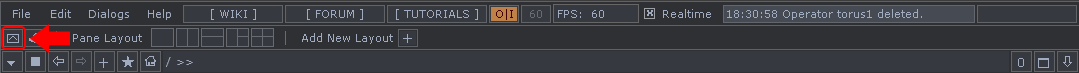
\includegraphics{./img/10.1/perform.png}
\end{center}

\end{fullwidth}

%------------------------------------------------

\section{Performing with the Network Editor}

\begin{fullwidth}

Every situation is different, and it is possible that programming might have to be done during a live performance. If that is the case, there are a few things that can help manage the impact the Network Editor has on the system. The first is to turn off the viewers on any Operators that don't need to be monitored. See the diagrams below:

\begin{center}
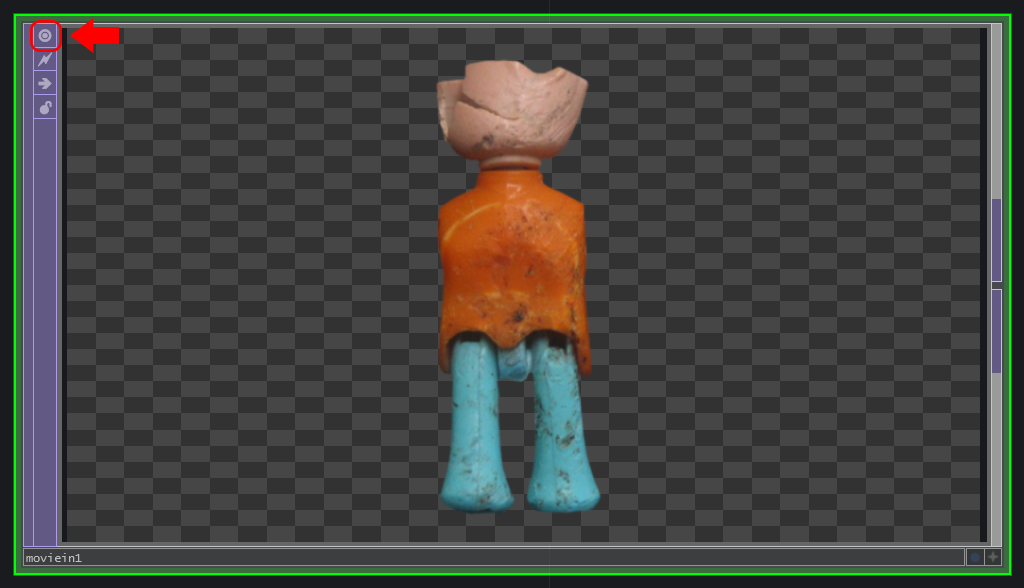
\includegraphics[width=12cm]{./img/10.2/performing-network-1.png}

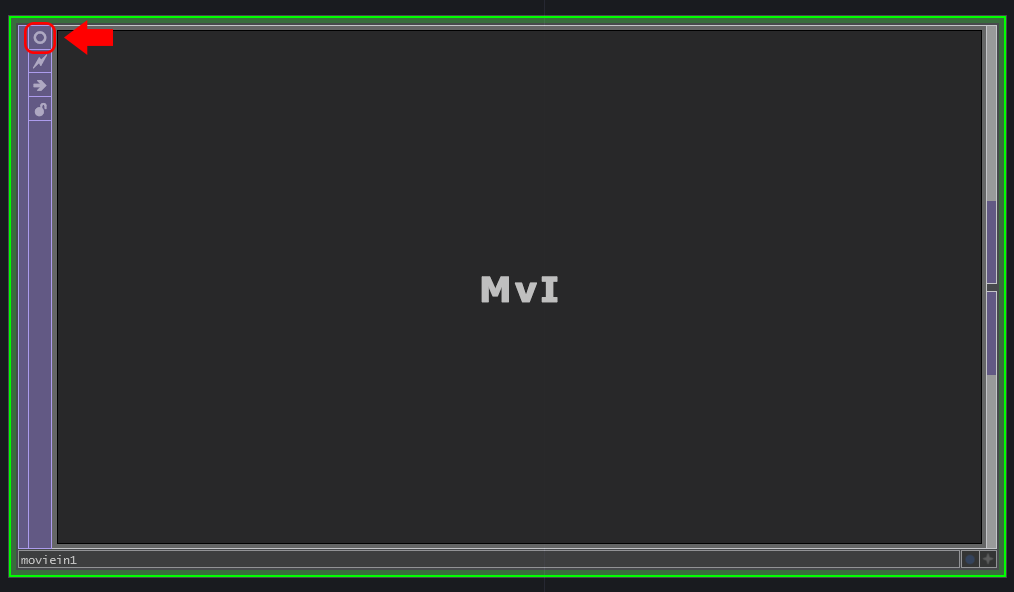
\includegraphics[width=12cm]{./img/10.2/performing-network-2.png}
\end{center}

The next thing that helps is to only use 1 pane in the Network Editor. The more panes that are visible, the more things there are needing to be rendered. 

Finally, moving in and out of large Networks should be avoided. Moving in and out of large Networks can cause frame drops, as TouchDesigner will have to render all of the Operators in that Network before they can be viewed. 

\end{fullwidth}

%------------------------------------------------

\section{Creating an Output Raster}

\begin{fullwidth}

As a general rule, to get the best performance possible, one should always strive to only use 1 Window COMP at a time. This doesn't apply while programming, but when it comes to deployment and performance, having more than one window open will greatly decrease the systems performance. So what should be done if there are multiple outputs with different positions and rotations?

The answer is to create a raster for the output and create a single, all-encompassing, window that will span all of the real-world outputs.

This is more simply expressed with an example. In this example scenario, there are four SXGA+ projectors, each with a resolution of 1400x1050. In the real-world setup, there are two projects beaming horizontally on side walls, and two projectors beaming vertically, and edge blended, on the center wall. The diagram below illustrates the desired setup.

\begin{center}
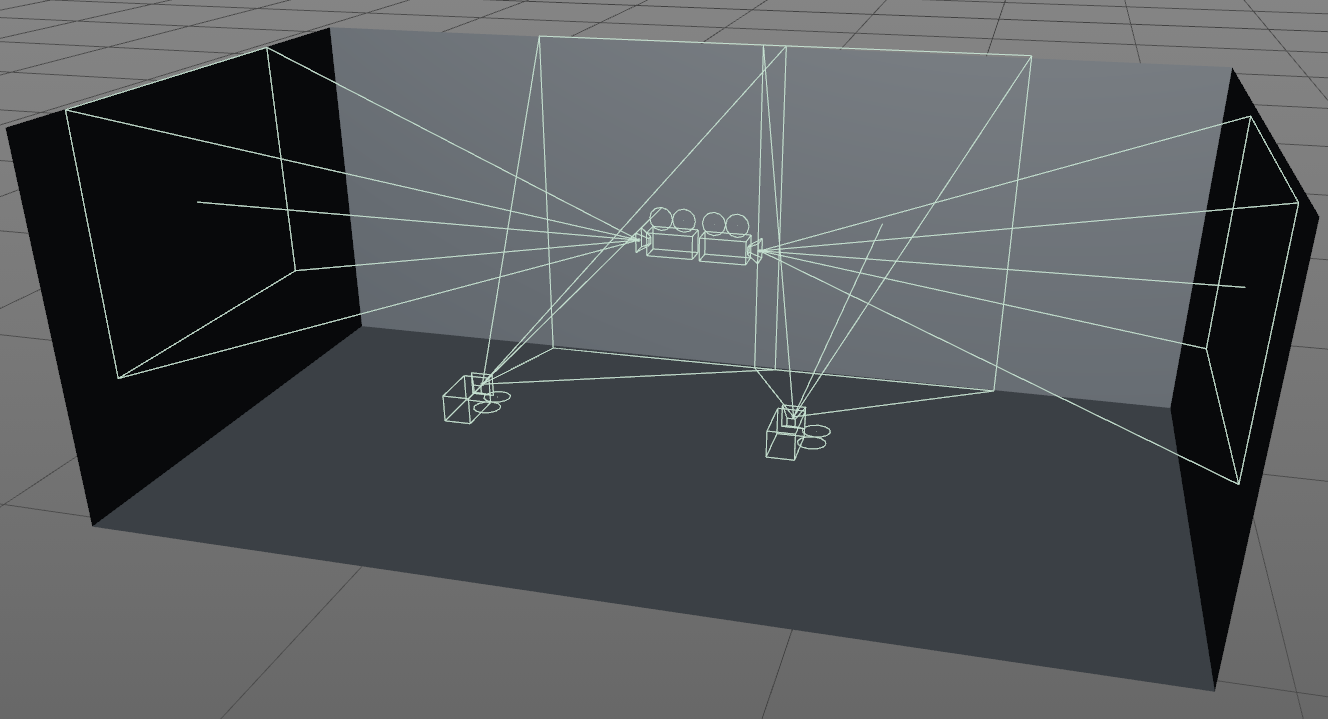
\includegraphics{./img/10.3/raster-1.png}
\end{center}

This setup isn't particularly complex, thus knowing how to deal with it most effectively is important. Let's take this setup, and lay it out in 2D. 

\begin{center}
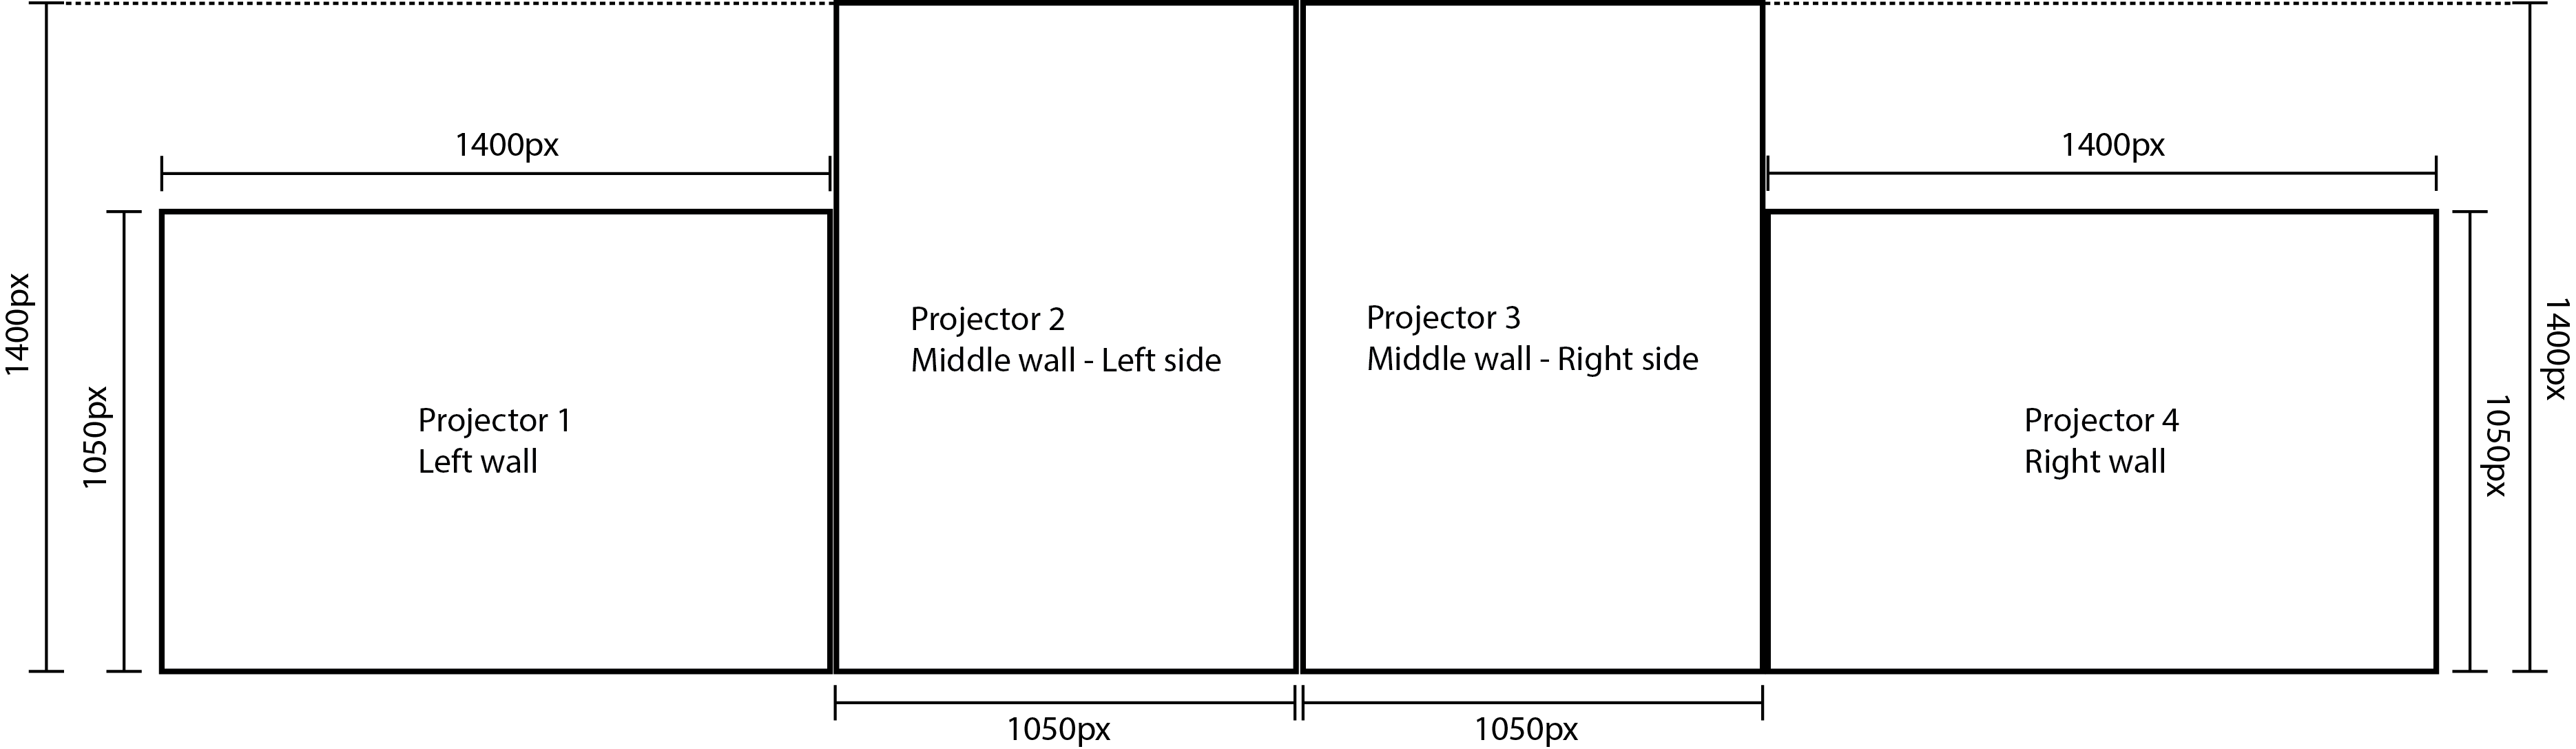
\includegraphics{./img/10.3/raster-2.png}
\end{center}

A beginners's first instinct might be to use four Window COMPs because there are four outputs, two of which need to be rotated. The challenge is finding the most efficient layout for these four canvases, to create a single raster. In this instance, because all four outputs are the same resolution, an easy solution is to make a 2x2 grid. 

\begin{center}
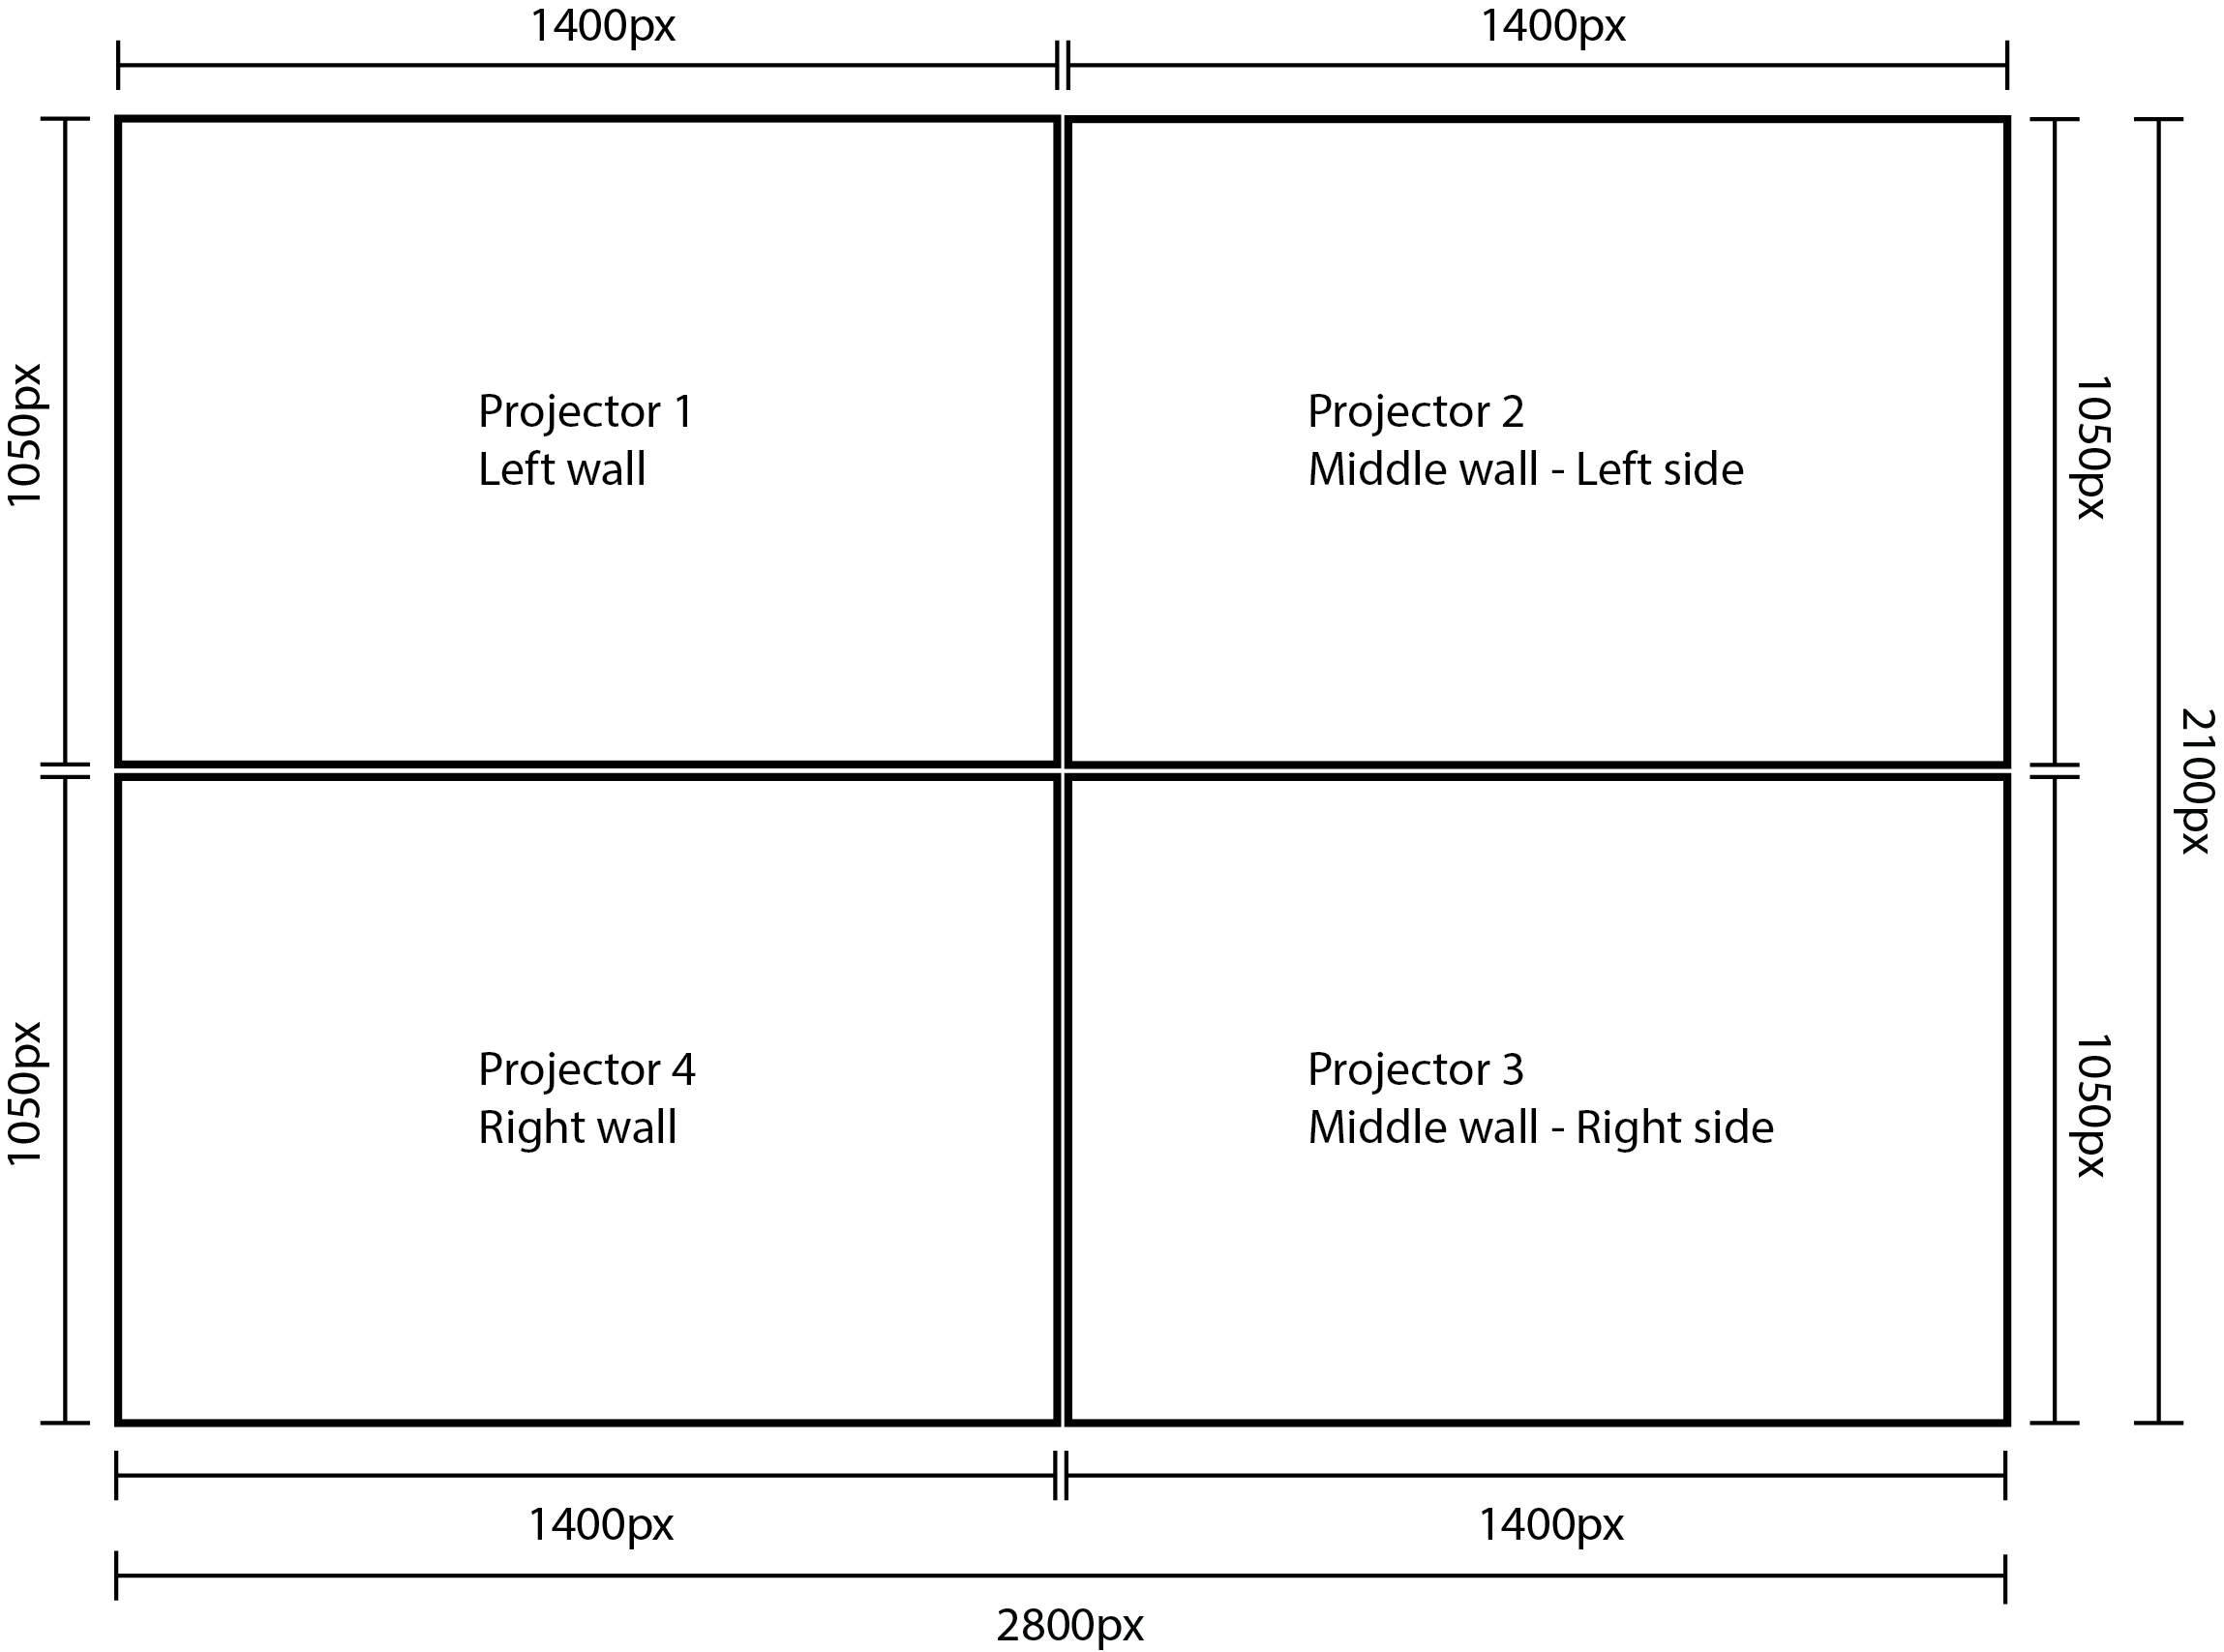
\includegraphics{./img/10.3/raster-3.png}
\end{center}

In the above diagram, all of the outputs are placed into a single raster. This setup can efficiently use one Window COMP that is 2800x2100 pixels. At this point, the nVidia or AMD control panel should be used to create a similar setup out of the monitors in Windows, which should then be connected to the correct outputs on the graphics card.

The next step is to prepare this raster inside of TouchDesigner. Open example 'Raster.toe'. There are a few things to note from the start. For the example, some very basic dummy content has been created, and will represent where real content would go. 'Content1' is for the left wall projector and is 1400x1050 pixels. 'Content2' is for the middle set of projectors and is 2100x1400 pixels. 'Content3' is for the right wall projector and is 1400x1050 pixels. All of the canvas building happens inside of the 'canvas' Container COMP.

In the 'canvas' container, the signal path can be followed from left to right, and from top to bottom, like a waterfall. The first step is to create a blank raster that content can be composited on. There is a Constant TOP set to 2800x2100 pixels at the top left of the Network for this purpose. Using an Over TOP, the first piece of content is placed, for the left wall projector, in its appropriate position, according to the diagram above. This is done using the 'Translate' parameter of the Over TOP. Projector 1: done!

The middle wall has two projectors that are edge blended together. Because a few operations need to happen on the raw content, there is a container name 'crop'. This keeps the operations encapsulated, neat, and easy to find. Inside of 'crop', three main operations are performed. The first is that the big piece of content is cut it in half, so that each projector can display half of the image. Since the projectors are positioned vertically in the installation, but are positioned horizontally in the raster, the 'Flop' parameter of the Flip TOP is used to turn the canvas on its side. The settings for the Flip TOP will always end up being different depending on hardware setup, so be prepared to try different Flip and Flop settings to get the correct content orientation.

Side note: Most beginners have trouble rotating a full canvas. The first instinct is to use the Transform TOP, but it is important to note that the Transform TOP will transform the pixels inside of a canvas. This is where the 'Flop' parameter of the Flip TOP comes in. It will fully rotate the canvas.

Since this example isn't dedicated to edge blending, the 'edge\_blend' containers are just place holders that create the visual effect of a blended edge. 

With all the cropping, rotating, and blending done, the two projector outputs are ready to be composited onto the raster. Using the same technique as before, an Over TOP with a modified 'Translate' parameter correctly positions the two pieces of content. Now Projector 2 and 3 done as well!

The final projector is as simple as the first, and using the trusty Over TOP, the final piece of the puzzle is positioned.
 
As mentioned in an earlier chapter, it is best practice to use Container COMPs instead of TOPs as the source for Window COMPs. In this project, there is a container that is 2800x2100 pixels that holds the completed raster. The 'final' container is set as the Window COMPs 'Operator', the 'Borders' setting is turned off in the Window COMP, and the window size is set to 2800x2100 pixels. With that, the project is ready to be output to the above, 4 projector, setup.

\end{fullwidth}

%------------------------------------------------

\section{Displays, Tearing, and Stuttering}

\begin{fullwidth}

There has not been much hardware discussion throughout this book, but it is important to keep a few things in mind when working with multiple displays. The most important rule is to always try to have all display hardware be exactly the same. Any difference in the signal flow, can cause what is called 'tearing'. The image below is an example of a frame that has tearing.

Examine the image below. Is it an example of what a frame with tearing will look like. Notice the two horizontal cuts across the frame:

\vspace{10mm}

\begin{center}
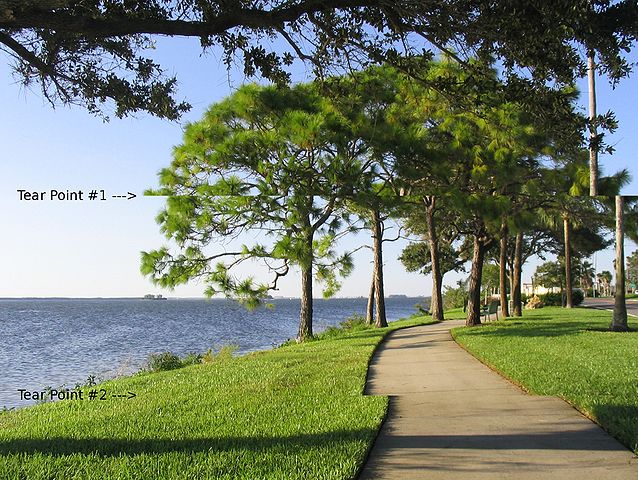
\includegraphics{./img/10.4/tearing.jpg}
\begin{footnotesize}
Image courtesy of Wikipedia
\end{footnotesize}
\end{center}

Tearing occurs when a display refreshes its image out of sync with when the graphics card renders its image. The result is part of the image being from the previous frame, and part of it being from the next frame. On slow moving content, this can sometimes be hard to notice, but once there is any sort of motion in the content, tearing becomes incredibly distracting.

Tearing is a complex issue to solve, but there are a few preventative measures that can be taken to avoid it. The first is to use a professional graphics card, such as something from the nVidia Quadro series. Most companies will not guarantee tear-free playback on anything but their professional cards.

The second is to always ensure that the displays are identical. Identical can't be stressed enough. If there is an installation with 3 outputs that have a refresh rate of 60hz, and one output with a refresh rate of 59hz, there is a chance there will be tearing. If there is an installation with two 1080p projectors, and two SXGA+ projectors, there is a chance there will be tearing. The best practice is to use displays that are not only identical in specifications, but are also the exact same model of displays. Network remote access applications like VNC and LogMeIn have also been the culprits of tearing.

This brings up a very important issue with tearing: there are no hard and fast rules. Sometimes, setups with a handful of different resolutions and refresh rates will work perfectly and won't tear. On the other hand, sometimes even setups with identical displays can tear. Enough emphasis cannot be put on preventative measures to avoiding tearing. When tearing issues arise, the only things that can be done are a step by step breakdown and analysis of the system to see what is causing the tearing.

There is a list of common debugging methods on the Derivative Wiki page for 'Tearing'. 

Generally the steps to begin with are as follows, in no particular order:

\begin{itemize}
\item Verify the project isn't dropping any frames. Dropped frames can sometimes trigger tearing
\item Verify no other applications are interrupting or mirroring the graphics card drivers, such as VNC and LogMeIn.
\item Disconnect every display connected to computer, and one by one connect them until tearing occurs. Then isolate that display on it's own, and figure out if it's being cause by a single display, or by the layout
\item Verify all displays are configured to the same resolution, colour bit depth, and refresh rate, in the nVidia or AMD control panel
\item Verify that none of the displays have any rotation applied in Windows. this can cause unpredictable behaviour.
\item Check the graphics card driver version and update it if necessary
\item Check for drivers or firmware updates on external video splitters - such as the Datapath X4 or Matrox TripleHead2Go
\item Confirm only 1 Window COMP is being rendered
\item Verify Windows Aero is disabled. In Windows 7, Aero can cause dropped frames and stutters, but won't tear. Once disabled, the system might tear, but stutter free playback is guaranteed.
\item Configure a Premium Mosaic using the nVidia Control Panel to create a single logical display 
\end{itemize}

There are many instances in which a system that performs perfectly, and doesn't drop a single frame, will occasionally stutter. This may occur because of how displays and graphics cards negotiate different refresh rates. 

If a project is running at 30 FPS, but a display's refresh rate is 60hz, frame doubling has to be negotiated somewhere. Between the graphics card and the display, most of the time this negotiation is done transparently, but sometimes there can be issues. What can occur is that instead of negotiating a proper frame doubling for every frame, one frame might be displayed once, while the next frame is displayed for three frames. From the project's point of view, no time is lost and no frames were dropped, so it would not be reported in the Performance Monitor or Windows Task Manager. 

If it seems that this kind of issue may be occurring, use the 'FPS is Half Monitor Refresh' feature in the Window COMP. This informs the graphics driver that it should show each frame for 2 refreshes.


\end{fullwidth}


%----------------------------------------------------------------------------------------
%	CHAPTER 11
%----------------------------------------------------------------------------------------

\cleardoublepage
\chapter{Optimization}
\label{ch:11}

%------------------------------------------------

\section{Introduction}

\begin{fullwidth}
Is is incredible to think about the challenges that are overcome when working in real-time. All the hardware and software aside, there is an extraordinary amount of precision to real-time work. When working in a project at 30 FPS, every single thing that is processed, displayed, and created, must be done in a 33ms window. That's not even a tenth of a second! This window is even smaller when working at higher frame rates. A project running at 60 FPS only has 16ms to render every frame from start to finish.

Realizing how tiny the window of opportunity is, it is important to cherish every single fraction of a single millisecond. Wonder why Operators are taking a whole millisecond to cook. Become nervous and try to salvage every half millisecond possible, knowing that every millisecond makes a difference. These all require basic project analysis and optimization skills.

TouchDesigner uses the CPU and GPU heavily, and knowing how to figure out which is under more demand is an important skill. When faced with larger and larger Networks, knowing where the system is stalling, and how to optimize Operators to get around these pitfalls, can be the difference between successfully delivering and not delivering a project.

\end{fullwidth}

%------------------------------------------------

\section{Finding the Bottleneck}

\begin{fullwidth}

The computer as a whole can be thought of as a pipeline. The CPU, GPU, RAM, and hard drives, all work together to create the final product. They sometimes work independently, but often times they are reliant on each other, because they individually perform very specific tasks. In a pipeline, the system can only be as fast as the weakest link. Because of this dependant nature, one stage of the pipeline can stall a whole project, even if the rest of the pipeline is completely clear. This stall, or weak link in the chain, is referred to as a bottleneck.

An example of a pipeline with a bottleneck is a project that tries to render some basic 3D geometry and texture their faces with video files. This hypothetical project consists of 4 Box SOPs. Every face of the Box SOPs are textured with a 1920x1080 HAP Q movie file. The computer being used for this has 32GB of RAM, dual 8-core processors, a top of the line nVidia Quadro graphics card, and a single 5400-RPM hard drive.

When launched, this project just won't run on this system. Regardless of how much RAM, how many processors, and how expensive a graphics card, the project can't read that many HAP Q files from a single 5400-RPM hard drive. The computer will continually stall because the hard drive can not spin fast enough to read every single movie file simultaneously. HAP Q files are demanding on the hard drive, and no matter how powerful the rest of the computer is, the project will not run. The GPU can't begin to read movies from a hard drive, just as the hard drive cannot begin to process pixels. The hard drive, in this case, has become the bottleneck in this project's pipeline.

Generally there are three areas where bottlenecking occurs: the GPU, the CPU, and the hard drives.

The GPU is a pipeline in and of itself, and pixel shading is the stage that is likely to become a bottleneck. Whenever operating on pixels, using almost any TOP, the system demands more and more of the GPU's pixel shader. The higher the resolution, the higher the demand on the GPU. There is a 1:1 ratio between a TOPs resolution and it's GPU workload. If a TOP's resolution is reduced by a factor of two, its GPU workload is proportionally reduced. A quick way to check if there is a pixel shading bottleneck is to lower the resolution of all generator TOPs, such as Render TOPs and Constant TOPs. If there is an immediate increase in speed and performance, then it is clear that there is a pixel shading bottleneck. 

When the graphics card is overworked, seemingly random TOPs will start to have higher than normal cook times. This becomes apparent when looking in the Performance Monitor at the cook times of various TouchDesigner UI elements. If all of a sudden, the various UI elements are taking more than a millisecond to cook, the Network needs to be optimized to relieve the GPU of some of its workload. 

The CPU is second area where bottlenecks are experienced. Most Operators require the CPU to function, thus the CPU can quickly be overworked. CPU bottlenecks tend to be easier to track down, because the Operators that take a long time to cook are visible in the Performance Monitor. It is possible to measure how much CPU head room there is with the Hog CHOP. This CHOP does as it name implies, and hogs CPU processing power. The 'Delay' parameter is the amount of seconds that the Hog CHOP will add to the cook time of each frame. If a Hog CHOP is created and the project begins dropping frames, that means the CPU is the our bottleneck. 

All movie files use the CPU to decode data from their compressed state. Certain codecs use the CPU more than others, and reading many movie files simultaneously can use more CPU resources than one would imagine.

An overloaded CPU reacts similarly to an overloaded GPU, in that inconsistent results will appear in the Performance Monitor. Operators will have varying cook times. This is because their operations are started, but before they finish, the CPU is called to perform another process. The amount of time that the Operator spends waiting for the CPU to return to its process is what increases it's cook time. Unlike a GPU overload, a CPU overload will generally effect more than just TOPs.

Hard drives are the third area where bottlenecks occur. Specific operations can be demanding on hard drives, and it is easy to overlook high quality solid state drives (SSD) when preparing systems for deployment. Operations such as reading and writing movies can quickly exhaust a drive, depending on the codec used. This bottleneck will often appear in the Performance Monitor as a line item under a Movie In TOP that such as:

\begin{lstlisting}
Waiting for frame for 90 - E:/test.mov from harddrive
\end{lstlisting}

\noindent Where the number is the frame of the movie, and the path is the path to the movie file.

\end{fullwidth}

%------------------------------------------------

\section{Using the Performance Monitor}

\begin{fullwidth}
The Performance Monitor is a tool for analyzing the cook time of a frame. This is useful when trying to optimize and debug a project's performance.

There are three ways to access the Performance Monitor: 

\begin{enumerate}
\item 'F2' on the keyboard
\item 'Alt + Y' on the keyboard
\item Clicking 'Performance Monitor' under 'Dialogs' in the menubar at the top of the screen
\end{enumerate}

There are only a few buttons, and they perform simple tasks that are almost self-explanatory.

\begin{center}
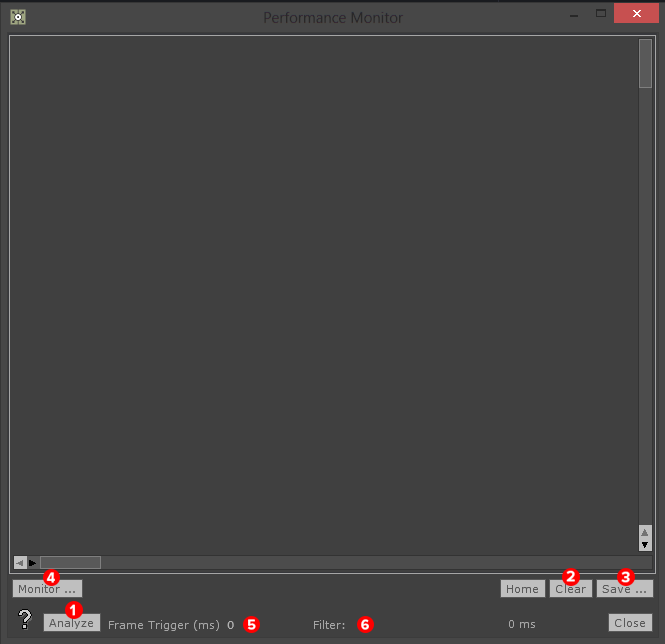
\includegraphics[width=11.5cm]{./img/11.3/performance-monitor-1.png}
\end{center}

\begin{enumerate}
\item Performs an analyses on the current frame
\item Clears the current results
\item Saves the current results to a text file
\item Change what is being monitored
\item A millisecond threshold value, which if crossed by a frame's cook time, will trigger the Performance Monitor to analyze
\item Filter the results for more precision, i.e. only CHOPS, TOPs, etc
\end{enumerate}

It is important to note that cook times are based on the CPU. This doesn't mean GPU bottlenecks will go unnoticed in the Performance monitor, but be cognizant that these are CPU readings. 

Here is an example analyses from the Performance Montior.

\begin{center}
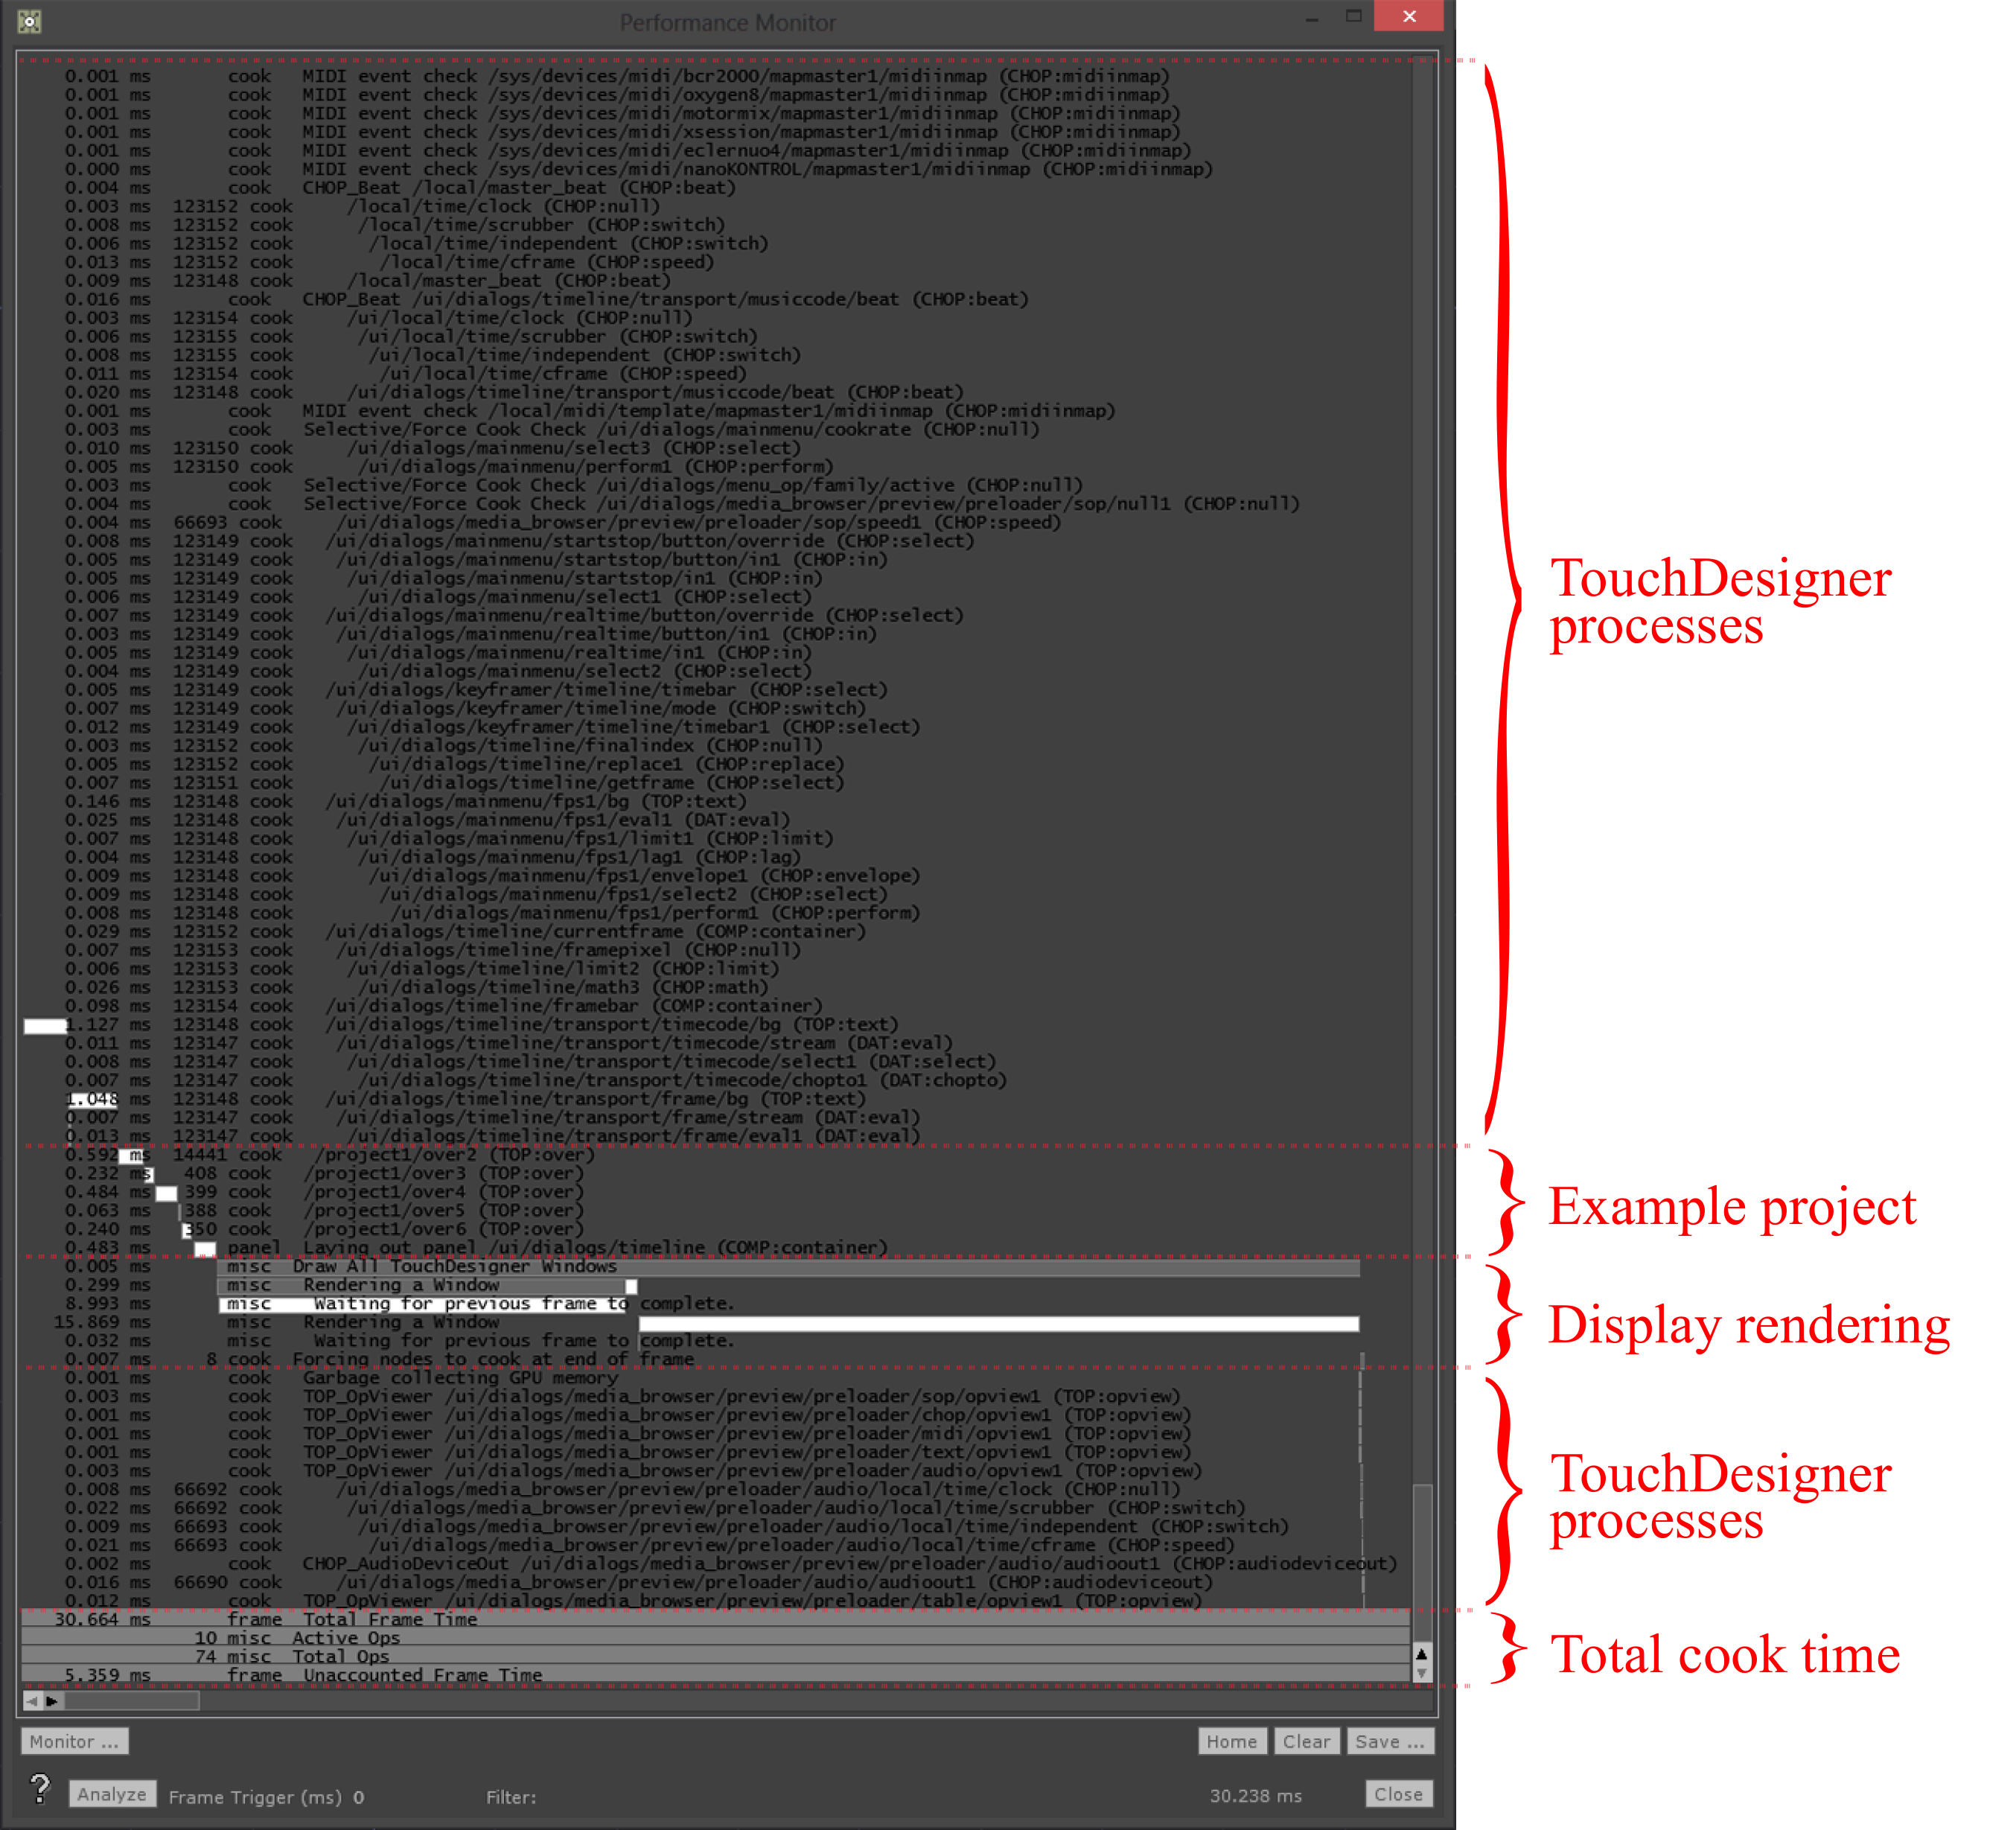
\includegraphics[width=14cm]{./img/11.3/performance-monitor-2.png}
\end{center}

The analyses above is taken from a simple project with a few Movie In TOPs and a few Over TOPs. Every frame that is analyzed will have some similar Operators. These are the Operators responsible for the functionality and user interface elements of TouchDesigner.

Look at the marked sections on the above diagram to see the cook times, and paths, for the Operators responsible for TouchDesigner's main functionality (User interfaces, dialog windows, etc), and more importantly the Operators belonging to the example project. The cook time of each Operator is represented by a white bar that is sized proportionally based on its contribution to the total cook time of that frame. When projects grow and become more involved, the section labeled 'Example project' will grow to include all of the project's Operators. This allows the analysis of a project to find problem Operators that too many system resources. 

In this example, the paths and cook times of the series of Over TOPs can be traced. They are all located inside of the 'project1' container, and their cook times range from 0.06 milliseconds to 0.6 milliseconds.  

A cautious side-note: Be careful of the effects of Vertical Sync and how cook time is perceived in the Performance Monitor. The graphics card will try to lock project FPS and display refresh rate. At 30 FPS, even in an empty project, the cook time per frame might be perceived as 33 milliseconds. The same effect can occur when working at 60 FPS, except that the Performance Monitor would show a frame cook time of 16 milliseconds. This doesn't mean that each frame actually needs a full 33 ms or 16 ms to render a frame, but that Vertical Sync is trying to sync TouchDesigner's FPS and the refresh rate of the displays. 

\end{fullwidth}

%------------------------------------------------

\section{Operator Cooking}

\begin{fullwidth}
Better performance can always be achieved by decreasing the amount of Operators that cook every frame. Many beginners never take this into account when creating Networks. Admittedly, everyone has worked on prototypes with tight deadlines, and has had to created Networks without much foresight. However, not taking cooking into account can be quite hazardous if a project can't afford any dropped frames.

The main goal is to perform static operations as early as possible in the signal flow, to prevent those specific from being rendered every frame.

Open example 'Cooking\_1.toe'. In this example, there is a simple graphic that rotates, and then various Operators are used to give the image a more interesting look. A feature that can help with optimizing Networks is the animation of the wires connecting Operators. Animated wires mean that the Operators on both ends are being cooked every frame. Starting at the far left of the Network, the wire between the Movie In TOP and the Transform TOP is not animated. This is because the image is loaded, and remains static. Operators only cook when they need to perform an operation or change. A still picture is static, and therefore does not change, and does not cook every frame. 

On the contrary, the rest of the wires in the Network are animated, meaning that everything after the Movie In TOP is cooking every frame. For this project, this isn't a dire problem, because there isn't anything extremely complex happening. Getting in the mind set of making efficient Networks from the start can save a lot of headaches come performance time. Let's take a look at this project in the Performance Monitor. 

\begin{center}
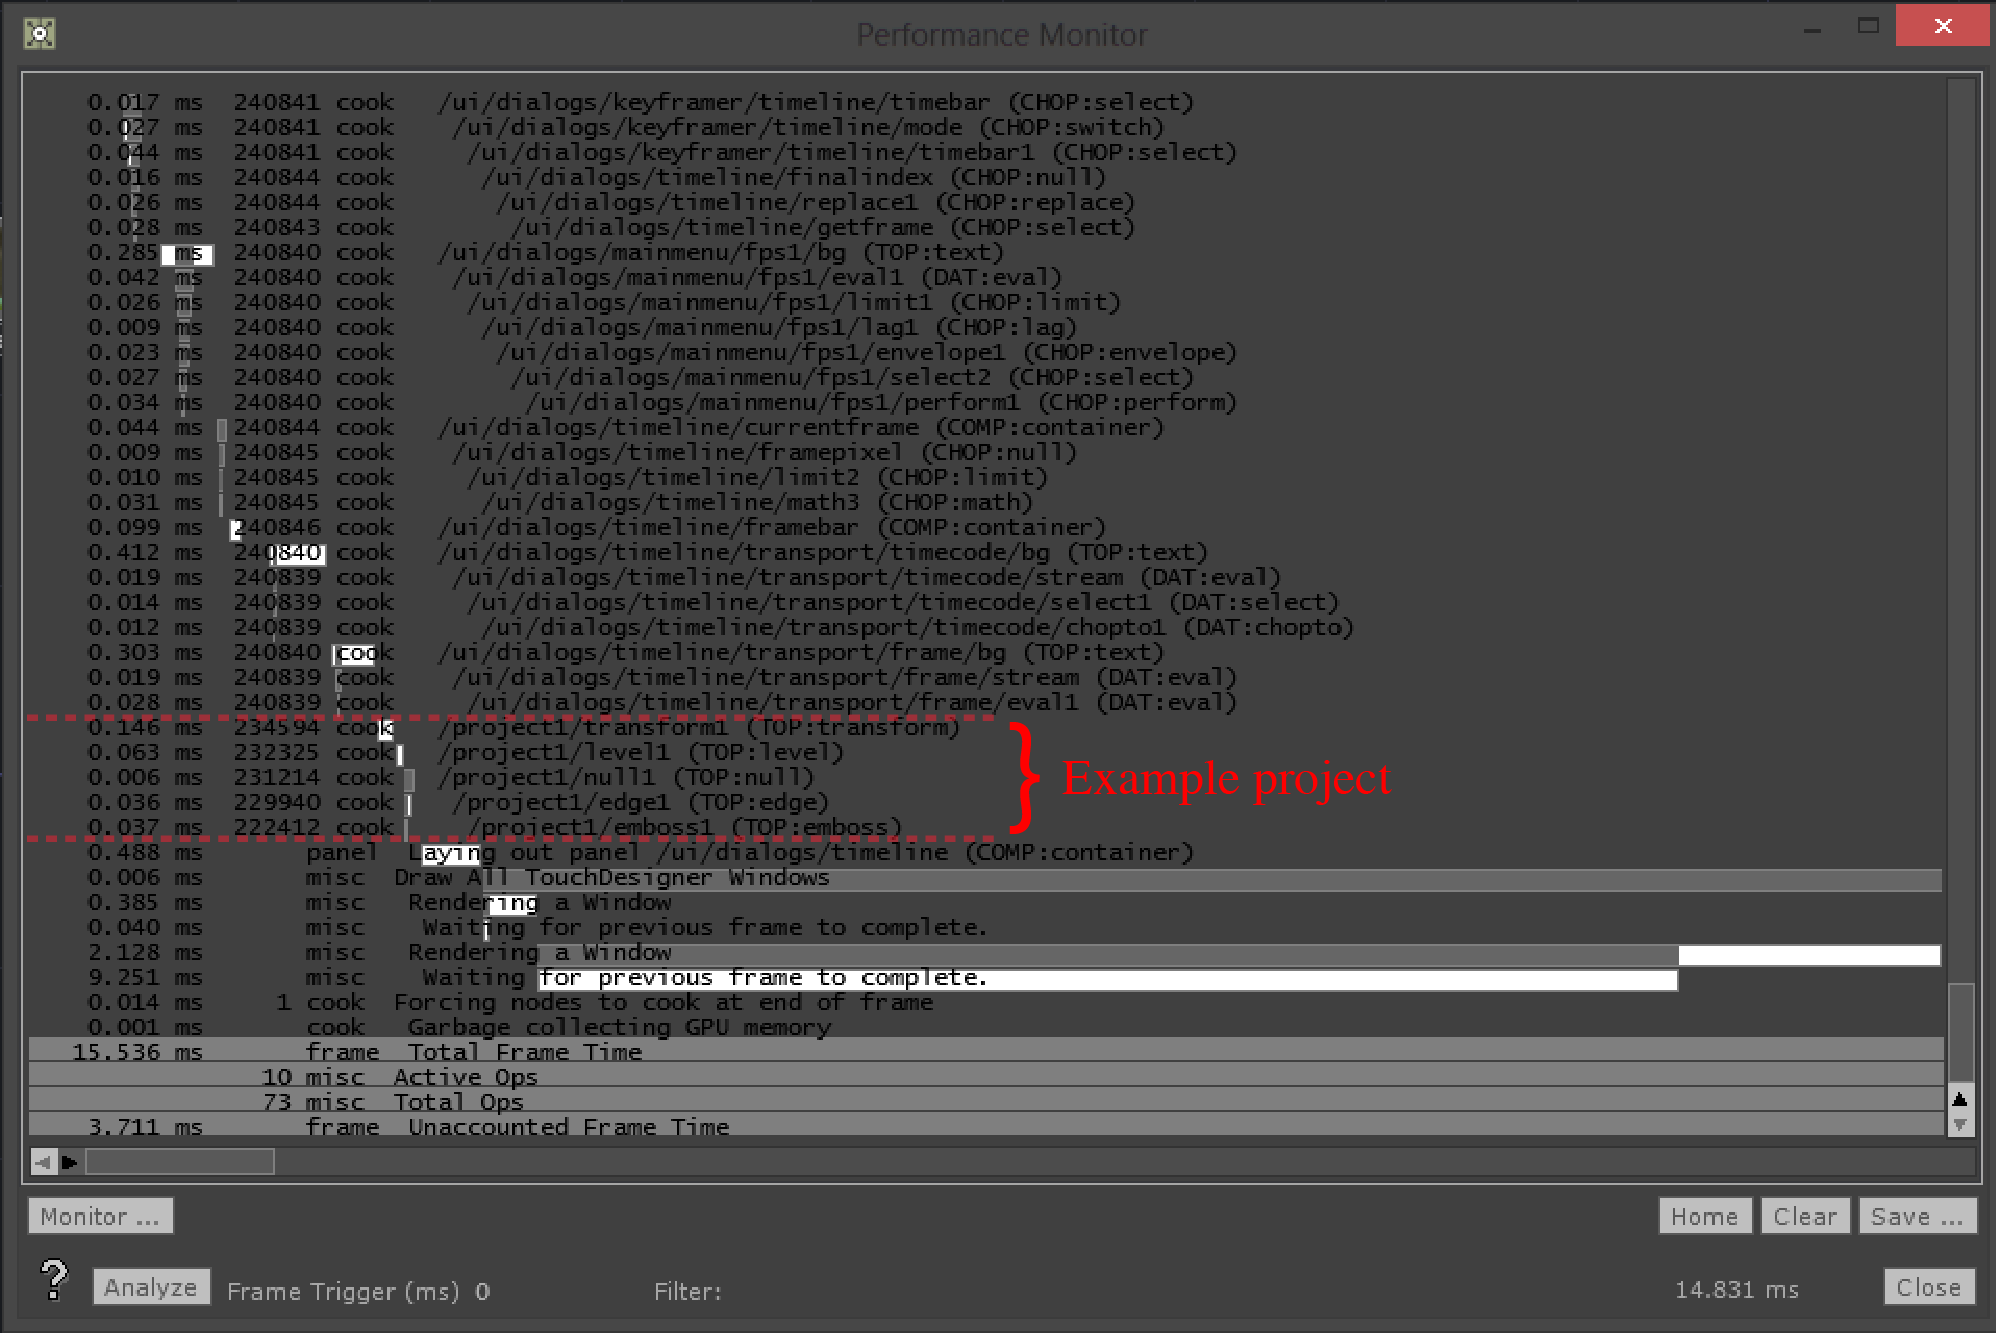
\includegraphics[width=12cm]{./img/11.4/operator-cooking-1.png}
\end{center}

Ignoring all the Operators needed for TouchDesigner's functionality, there is a small block of Operators dedicated to this example. The operations being performed on the image, in total, take about 0.25 milliseconds. As mentioned, static operations only need to cook once, and something to note is that many of the operations after the Transform TOP are  static in nature. Let's re-arrange these and see the gains in performance.

Open example 'Cooking\_2.toe'. This project is the same as the previous, except the Operators have been re-arranged. Before examining the signal flow closer, let's take a look at the Performance Monitor.

\begin{center}
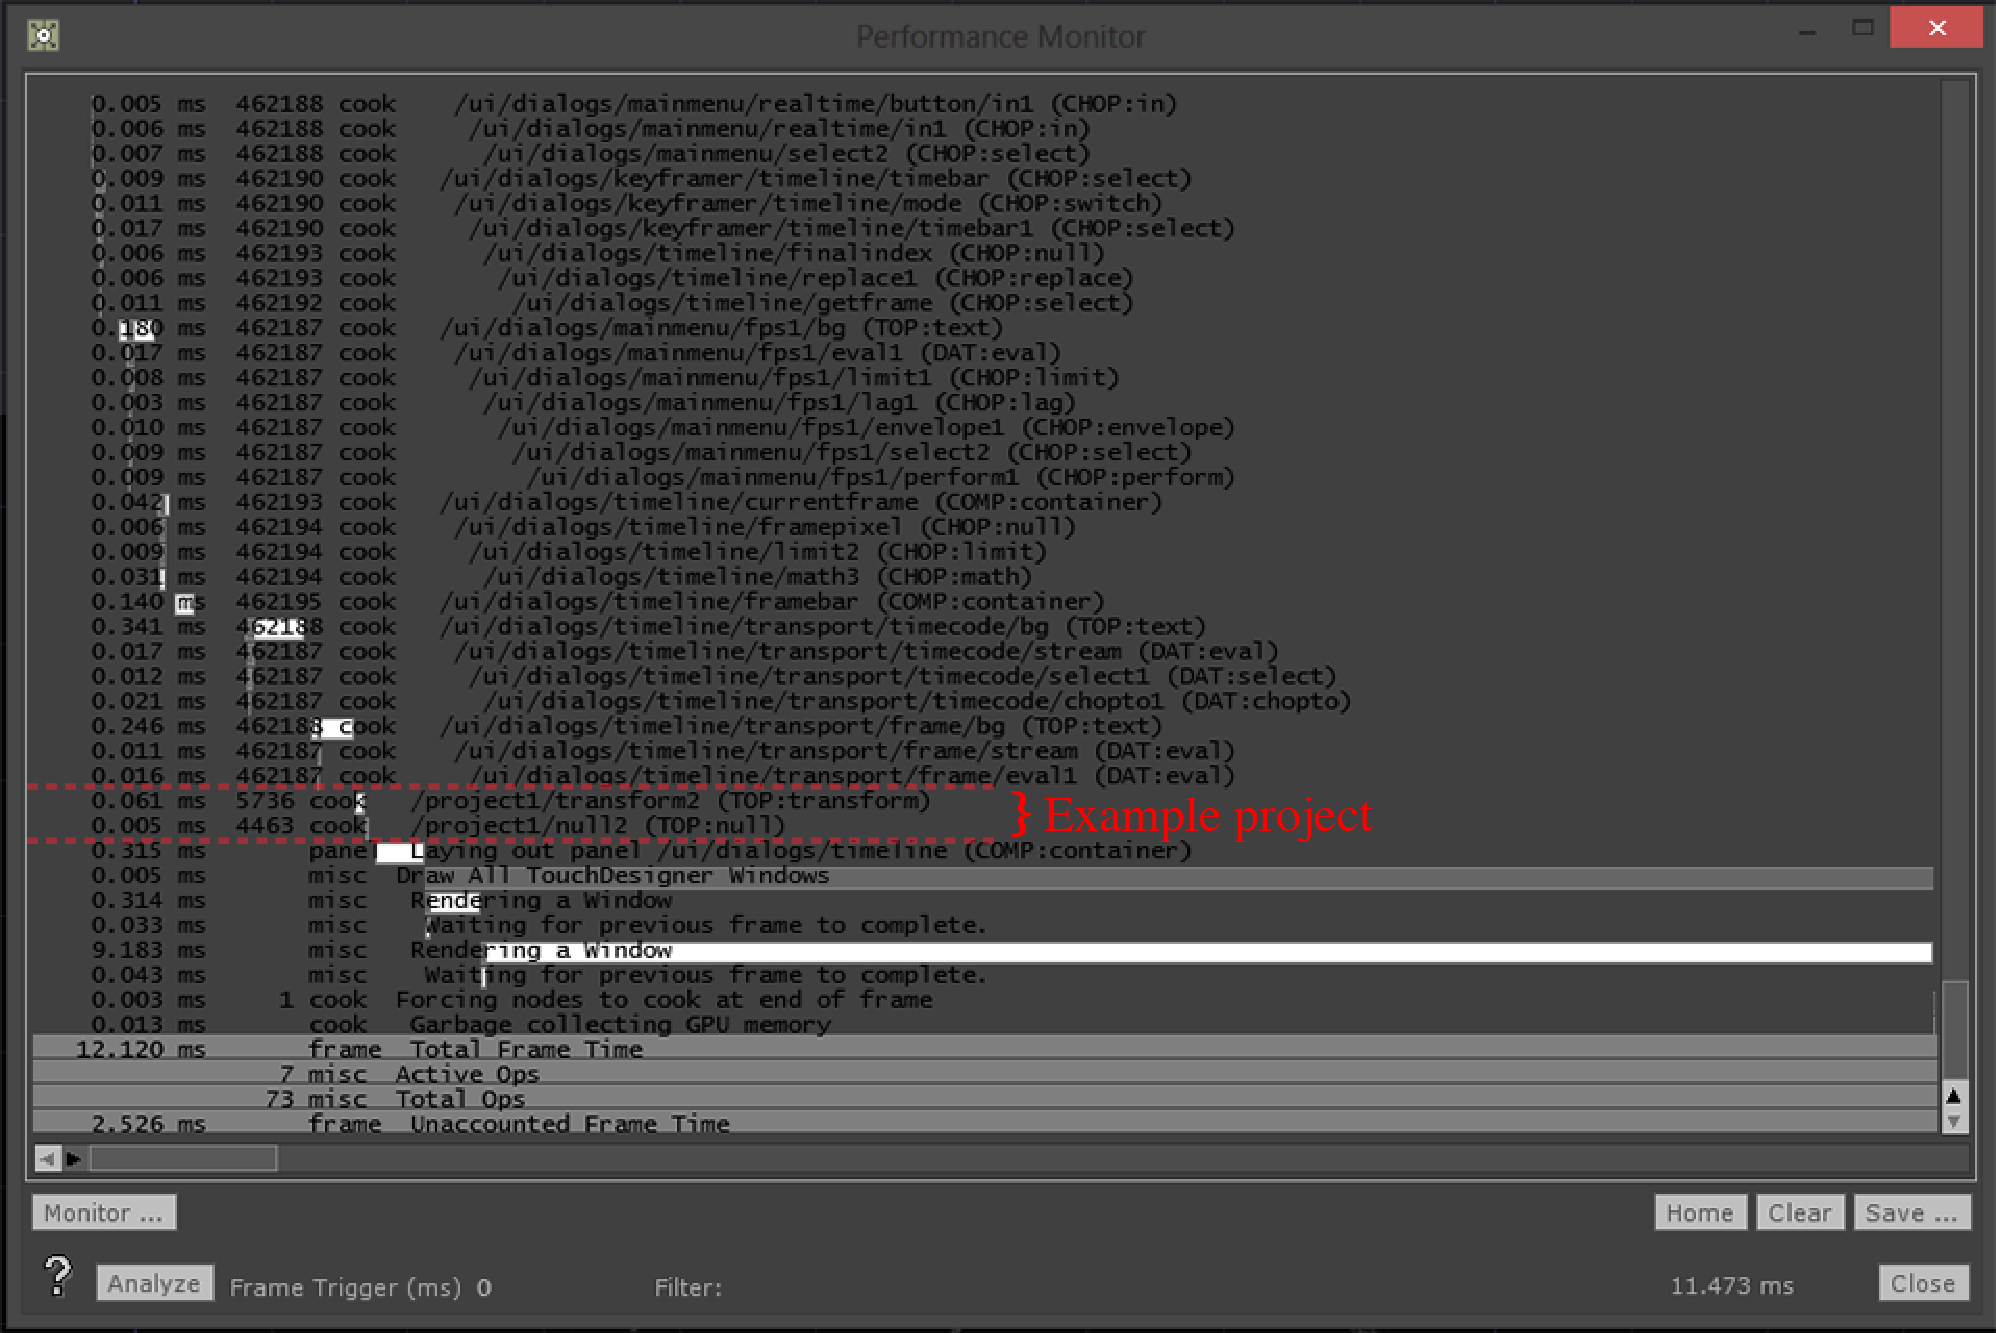
\includegraphics[width=12cm]{./img/11.4/operator-cooking-2.png}
\end{center}

At first glance it appears as if the project has shrank! A few of the Operators that were listed previously have disappeared. This is because these Operators aren't cooking every frame. In the last example, the Transform TOP was performing a transformation every frame, forcing the TOPs after it to recalculate their operations every frame. In this example, all of the static operations happen at the start of the signal flow, leaving the Transform TOP free to perform its transformation, without forcing any other Operators to recalculate their operations, or cook.

Taking a more in depth look at the Performance Monitor reading, the only Operator that was cooked was the Transform TOP, which took 0.061 milliseconds to cook. Compare this to the previous example, where the series of operations took 0.25 milliseconds to cook. That is an unbelievable gain for such a simple change.

It is worth noting that side by side, the outputs of these two Operator chains may not be exactly identical, but they are so indistinguishable from each other that many clients and artists will not mind the difference, knowing that the massive performance gains will allow them to do so much more.

\end{fullwidth}

%------------------------------------------------

\section{Resolution}

\begin{fullwidth}

When it comes to working with 2D textures, resolution is extremely important, because of the almost 1:1 ratio of pixels processed compared to processing power used.

An incredibly easy way to demonstrate this fact is through example. Open example 'Resolution\_1.toe'. This is a simple setup. The butterfly is composited on a bigger canvas, then using some LFOs, the opacity and blur are modulated before it is composited onto the forest background.  Middle clicking on any of the TOPs will reveal that this example requires just over 100MB of GPU RAM. That's not a lot of memory on a system with 4+ GB of GPU RAM, but this can quickly add up. Try to composite 40 of these butterflies in real-time, and 4GB can easily be spent. 

Now contrast this to example 'Resolution\_2.toe'. It creates the exact same results, but for only 60MB of GPU RAM. That is a significant difference. Take the above example of compositing 40 butterflies, and using this second method, only about 2.4 GB of GPU RAM are needed. All of the extra headroom from a simple change in resolution. The source butterfly asset is only 512x512 pixels, and in the first example, it is immediately composited on a 1920x1080 pixel canvas that is modulated. This creates a scenario where TouchDesigner is constantly re-drawing all 1920x1080 pixels every frame that the butterfly is modulated. 'Empty' pixels that have neither colour or alpha data are also re-drawn. In the second example, the exact same operations are being performed, but only on the source asset, which is a much lower resolution. This modulated asset is then composited on the 1920x1080 canvas. This saves the GPU having to re-draw a large canvas of pixels, when only a small section requires processing, thus saving quite a bit of GPU RAM and processing power.

\end{fullwidth}

%------------------------------------------------

\section{GPU Memory Fragmentation}

\begin{fullwidth}

Operators that use the GPU will often allocate the resources required for their tasks, and hold onto them until the task has been completed or changed.

GPU Fragmentation is one of the main concerns when working working with projects that have many different content sources. For example, a Constant TOP with a resolution of 1280x720 is connected to 10 other Operators. Once connected and cooked, each Operator will set aside the proper amount of GPU memory required to handle the processing of its specific amount of pixels. Once the memory is allocated, the Operators can operate relatively efficiently within their allocated space.

If the resolution of the source Constant TOP is changed, this will trigger a chain reaction, where all of the 10 other Operators will have to reallocate the correct amount of GPU resources for their tasks. If the Operator's resources are reallocated efficiently, many of the same memory blocks will be reused. If on the off-chance they can't reuse memory blocks, they'll have to relocate to the end of the memory. If this happens enough times in quick succession, the GPU memory will be fragmented, leaving the project in a state of poor performance while the GPU tries to defragment it's memory.

The two diagrams below try to outline memory fragmentation in the simplest way possible.

There are two case studies, both with similar parameters: There are 3GB of GPU RAM and there are three 1GB static textures to load and hold in RAM indefinitely.

\begin{center}
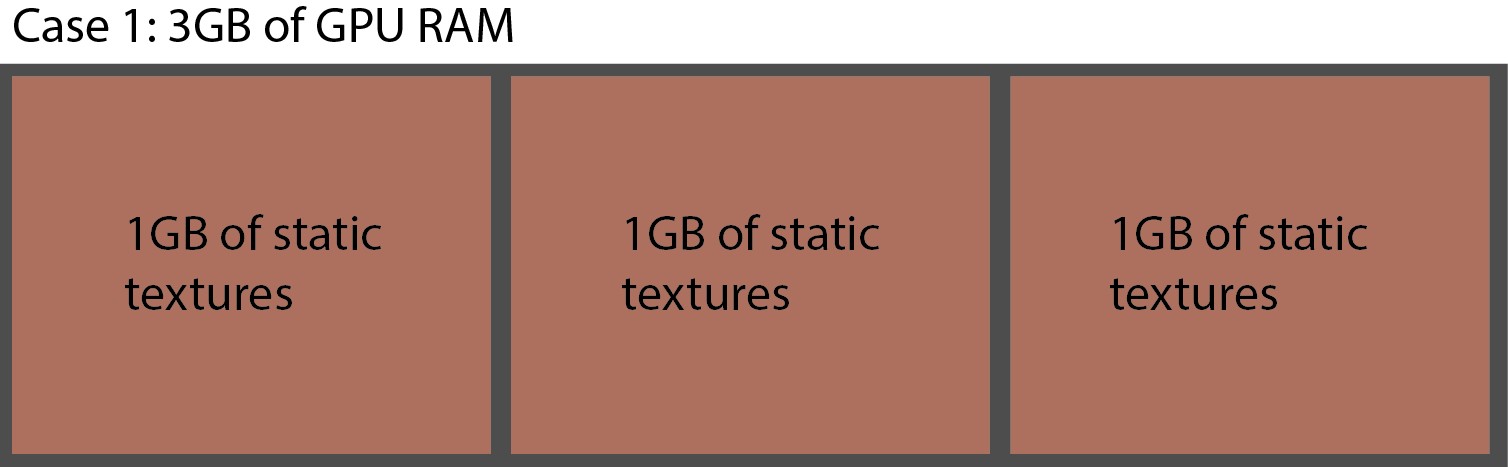
\includegraphics{./img/11.6/memory-frag-1.png}
\end{center}

In Case 1, the 3GB GPU of RAM would be able to perfectly fit the three 1GB static textures. They are called static textures because once they've allocated to memory, they aren't changed. This is the equivalent to loading a large image into a Movie In TOP at the start of a project and leaving it there indefinitely.

This is a perfect world situation, as there are many other processes that use GPU RAM, meaning resources are constantly in flux, and there would never be 3GB of free RAM on a graphics card that only has 3GB of GPU RAM.

Case 2 describes a situation where memory fragmentation will occur. To the already existing three 1GB textures, a 200MB texture is added to the mix. In this example, the loading and unloading is to happen in the following order:

\begin{enumerate}
\item Load 1GB texture
\item Load 200MB texture
\item Load 1GB texture
\item Unload 200MB texture
\item Load 1GB texture
\end{enumerate}

This would simulate a situation where a texture is loaded, displayed, and then replaced with another texture. 

\begin{center}
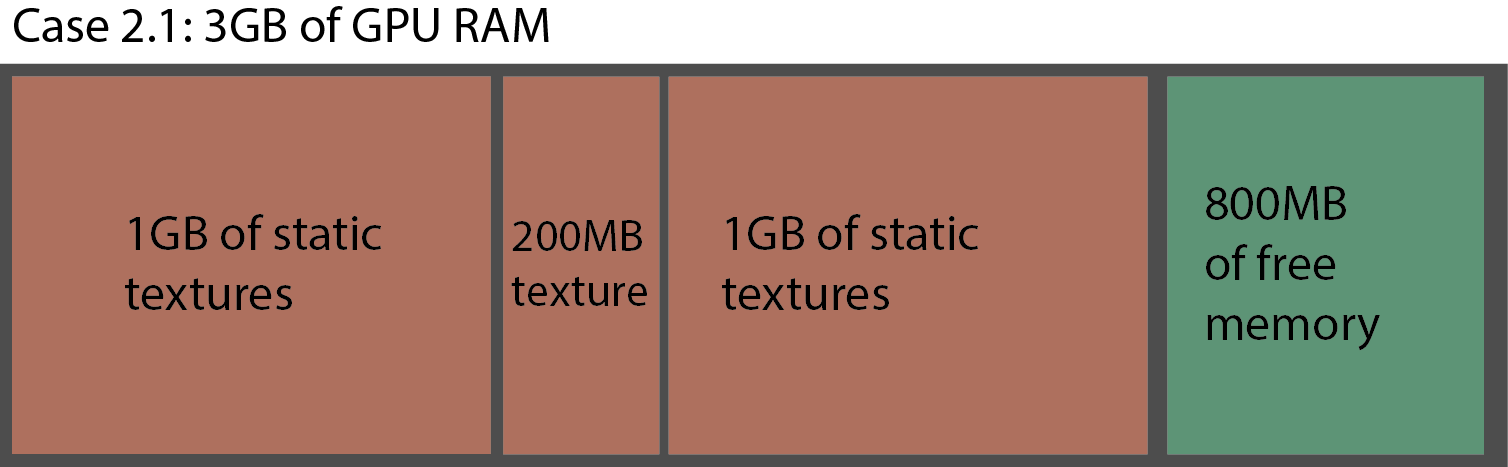
\includegraphics{./img/11.6/memory-frag-2.png}
\end{center}

In diagram 'Case 2.1', Steps 1 through 3 are completed, and there is 800MB free. At first glance, this might seem perfect, because if the 200MB texture is unloaded, there would be 1GB of free space for the final texture. Unfortunately, this isn't how graphics cards work.

\begin{center}
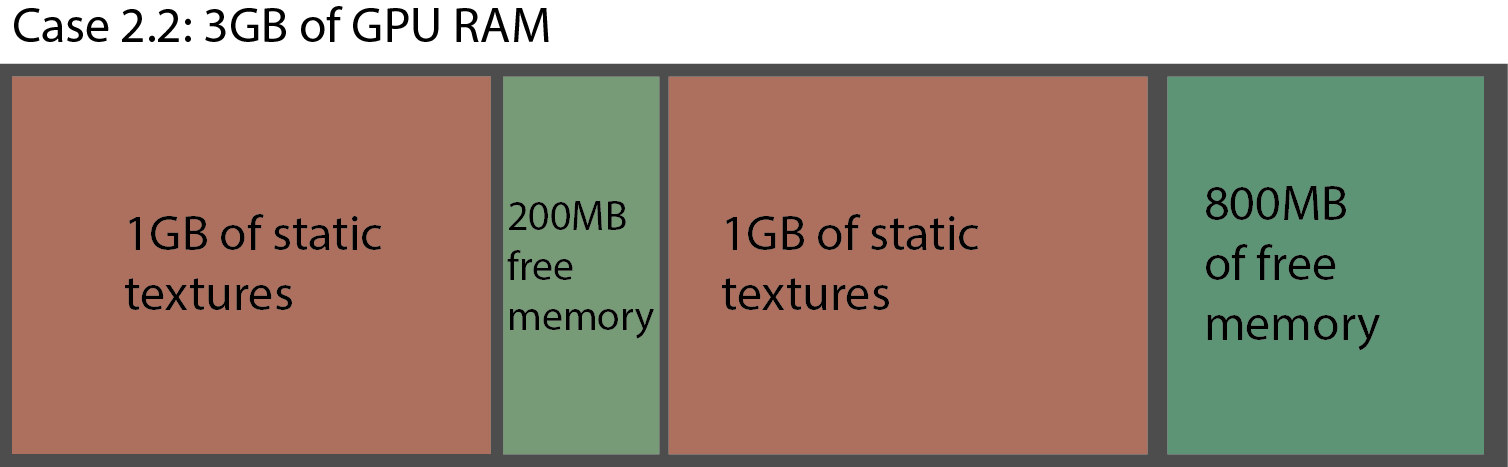
\includegraphics{./img/11.6/memory-frag-3.png}
\end{center}

As seen above, in diagram 'Case 2.2', Step 4 has been completed, and the 200MB texture has been unloaded. What remains is a prime example of GPU memory fragmentation. There is a total of 1GB of free GPU memory, but there isn't a single block of 1GB to allocate to the 1GB texture. The already-loaded 1GB textures, in their static state, can't be shifted in the GPU memory without a full unload and reload process occurring, and because the memory can't be shifted, the 200MB of free space has been trapped between the static textures. This 200MB allocation can be filled with 200MB or smaller textures, but it will not be able to load the third 1GB static texture.

The best way to prevent heavy memory fragmentation is to try to and restrict the amount of varying resolutions in a project. When an asset is swapped out for one that is the same resolution, often times it can take it's place in the memory.

\end{fullwidth}

%------------------------------------------------

\section{Windows System Processes}

\begin{fullwidth}
Windows is a complex operating system, and there are many processes and system-related applications running behind the scenes. Many of these processes and applications can negatively impact performance of a computer, and TouchDesigner. 

Windows is made for a large market of consumers, who primarily use their computers during the day. Because of such, there are many applications and Windows system operations that are scheduled to run if a computer is left powered-on overnight. This can be problematic for performance installations that run 24 hours a day. Depending on the needs of the installation or performance, many different applications and system related tasks can, and should, be turned off and rescheduled.

Applications such as virus and spyware scanning softwares, albeit useful for daily computing, should generally be avoided when using TouchDesigner. Virus and spyware softwares can cause a number of issues, the first being pop-ups. Many of these softwares display pop-up reminders and notifications at regular intervals. In unfortunate situations, these can overlap with displayed content and cover outputs during performances and installations. These applications can negatively effect the hard drive as well, as they often scan the system for viruses and malware, using up hard drive read \& write cycles. These two issues are aside from the CPU toll that many of these ever-running applications can incur. 

\end{fullwidth}

%----------------------------------------------------------------------------------------
% CHAPTER 12
%----------------------------------------------------------------------------------------

\cleardoublepage
\chapter{GLSL}
\label{ch:12}

%------------------------------------------------

\section{Introduction}

\begin{fullwidth}
GLSL, or OpenGL Shading Language, is an incredible tool to have in one's back pocket. With a little bit of code, one can program directly on the GPU.

Many avoid learning GLSL because they believe that it is only useful for working with large textures (4K and beyond), complex 2D generative visual scenes, or creating and manipulating 3D geometry, but it can be used in so many facets of day to day programming. Whether that be optimizing and creating incredibly effecient compositing workflows for standard HD content, or creating simple generative backgrounds for interactive experiences.

The goal of this chapter is to introduce the reader to some basic GLSL workflows and techniques, with the assumption that the reader has no previous GLSL experience.

\end{fullwidth}

%------------------------------------------------

\section{Types of Shaders and Rendering Pipeline}

\begin{fullwidth}
The two main types of shaders that can be programmed in TouchDesigner are the Vertex shader and the Pixel (or Fragment) shader. In a standard rendering pipeline, they are processed in that order, as can be seen in the diagram below:

\begin{center}
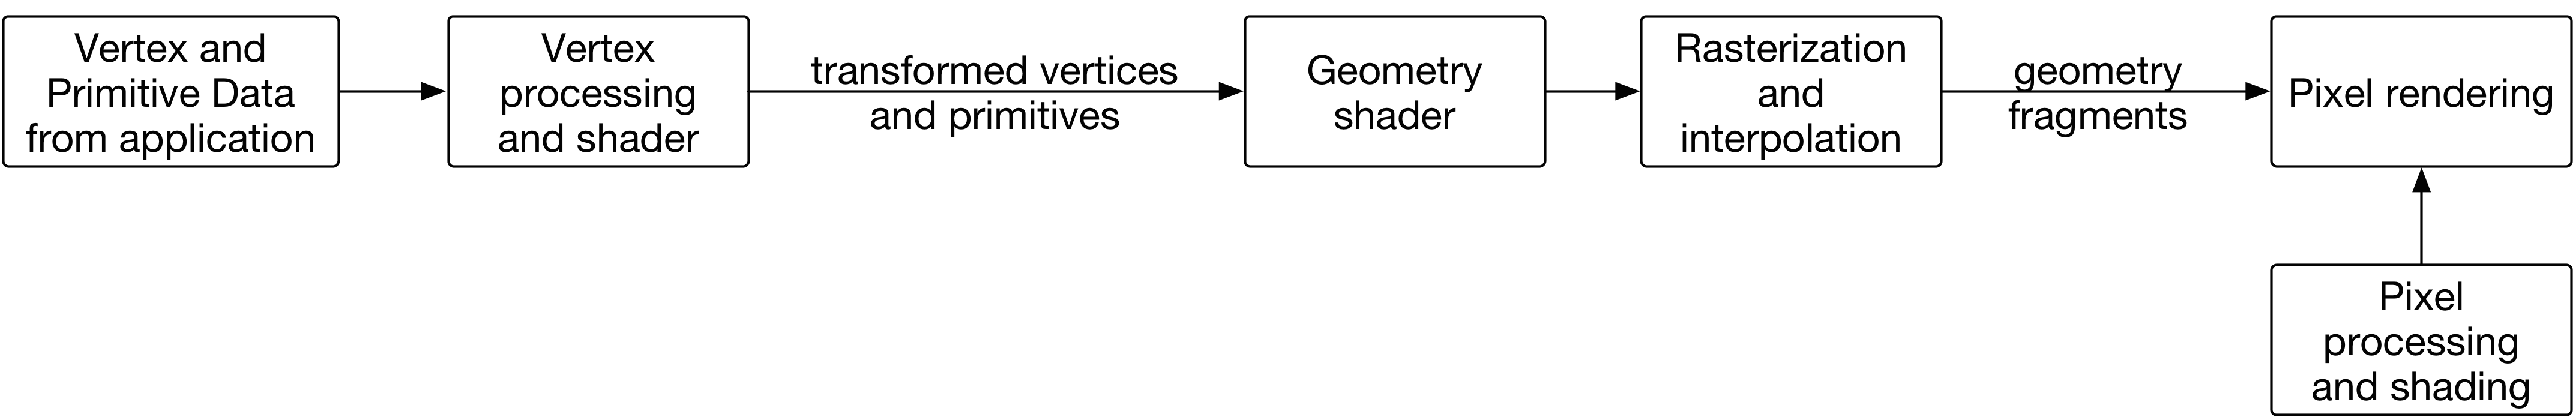
\includegraphics{./img/12.2/pipeline.png}
\end{center}

There is also a geometry shader that can be applied between the Vertex and Pixel shaders for layered rendering and transform feedbacks, but it is not used commonly.

In the above pipeline, the application passes the vertex and primitive data to the GPU. This includes information such as vertex position, texture coordinate, color, normal, etc. This information can be programatically processed and worked with by using a Vertex shader.

When the Vertex shader has finished processing the vertex and primitive data, the geometry is rasterized. During this process, the geometry goes through various stages such as clipping, culling, transformations to window space, etc. These stages prepare fragments that will be processed by the Pixel shader.

The Pixel shader takes these fragments, processes them, and outputs the color and depth data for each pixel.

For a more in-depth look at the render pipeline, there is a more thorough explanation on the OpenGL website:

\url{http://www.opengl.org/wiki/Rendering_Pipeline_Overview}

\end{fullwidth}

%------------------------------------------------

\section{Debugging}

\begin{fullwidth}
Before getting too deep into the world of GLSL, it is important to know how to debug compiling issues. There are two signs that denote a compiling error.

The first is a blue and red checker pattern. When working with the GLSL MAT, this check pattern will be on the geometry itself. When using GLSL with TOPs, this checker pattern will fill up the Operator's viewer and be output from the TOP.

The second sign of a compile error is a yellow triangle warning flag on the Operator. Upon clicking and holding the left mouse button on the flag, the error will read:

\begin{lstlisting}
Warning: The GLSL Shader has compile error
\end{lstlisting}

To diagnose these issues, an Info DAT is required. Create an Info DAT, and set the 'Operator' Parameter to reference the GLSL operator with the error. In the Info DAT, if there are no errors, there will be only a few lines and of them will read 'Compiled Successfully' or 'Linked Successfully'. If there are errors however, they will read more like:

\begin{lstlisting}
Pixel Shader Compile Results:
0(3) : error C0000: syntax error, unexpected '=', expecting '::' at token '='
\end{lstlisting}

To quickly break this down, the first thing is the line number. In this case, '0(3)' means the compiler is encountering errors at line 3. In many situations, this may mean that the actual mistake happens a line or two earlier, but the compiler doesn't halt until the next line when things stop making sense for it.

The next section highlights that this is a syntax error, and then there is more information about the error.

For beginners, the majority of these errors will be because of forgotten semi-colons at the end of lines, or errors trying to cast one data type into another incompatible data type.


\end{fullwidth}

%------------------------------------------------

\section{Shaders in 3D}

\begin{fullwidth}
Let's start by looking at a few very simple 3D scenes that utilize Vertex and Pixel shaders.

Open example 'Basic\_3D.toe'.

This is a simple render setup where the vertex shader does nothing but pass the vertices to the pixel shader, which then colors everything white. Let's take a more in-depth at each shader, starting with the Vertex shader:

\begin{lstlisting}
void main(){
	gl_Position = TDWorldToProj(TDDeform(P));
}
\end{lstlisting}

Since this is written for someone with no GLSL experience, a few notes about basic C syntax and rules that need to be followed, since GLSL is very similar to C.

The first thing is that semi-colons need to be added at the end of working lines of code.

The second thing is that most of the working code will be inside of the main() loop. For beginners, the only things outside of the main loops will be the delcaring of variables such as input and output streams and attributes.

When starting an empty shader, it's good practice to start by entering the main() loop as follows:

\begin{lstlisting}
void main(){

}
\end{lstlisting}

In this vertex shader, there is only have one line of code:

\begin{lstlisting}
gl_Position = TDWorldToProj(TDDeform(P));
\end{lstlisting}

Let's break this down from right to left, as there is a lot going on here.

'P' in this instance is the vertex position. In TouchDesigner, there are a few attributes that are declared by default. For instance, 'P' is the vertex position, 'N' is the normal, 'Cd' is the color, and 'uv' is the texture coordinate layers (it is an array that is accessed by index, i.e. uv[0], uv[1], etc). These values can be accessed as easily as we've accesed 'P'.

In the line of code, 'P' is input into a function named 'TDDeform()'. This function takes the vertex position from object space and returns the position in world space.

Think of object space as if each object in the 3D world had it's own co-ordinate system and 0,0,0 point. After processing these vertices, they have to be transformed and integrated into world space. World space is, as the name implies, the full world. The world, in this case, is the common coordinate system, with one 0,0,0 point, where all objects will exist together.

Once the vertex positions are returned in world space, they are passed to the function 'TDWorldToProj()'. This function takes the world space co-ordinates and returns them in projection space. The projection space takes all the co-ordinates from the world space, and returns them from a camera's point of view.

These values are then assigned to the variable 'gl\_Position', which is a built-in output for the transformed vertices.

As shown in the rendering pipeline diagram, these transformed vertices are processed and passed to the Pixel shader, where they will be assigned color values.

In this example, the Pixel shader sets the color output of all the fragments to white. The code is below:

\begin{lstlisting}
out vec4 fragColor;
void main(){
	fragColor = vec4(1,1,1,1);
}
\end{lstlisting}

Similar to the Vertex shader, all of the code except for the output declaration are inside of the main() loop, and there are semi-colons at the end of lines of code.

Starting from the top, there is this line of code:

\begin{lstlisting}
out vec4 fragColor;
\end{lstlisting}

This line sets the output as a variable called 'fragColor'. A 'vec4' is a vector with 4 components, and in this scenario, they correspond to the output red, green, blue, and alpha channels. In GLSL, whenever declaring an input or output, the type must be declared as well, thus the specification that it will be a 'vec4'. Similarly, inputs will be prefaced by 'in' and outputs will be prefaced by 'out'.

The line of code inside of the main() loop is as follows:

\begin{lstlisting}
fragColor = vec4(1,1,1,1);
\end{lstlisting}

As 'fragColor' has already been declared as the output, this line writes the pixel values directly to the output. The section 'vec4(1,1,1,1)' creates a 4-component vector with the values 1,1,1,1, and then assigns it to 'fragColor'. 'vec4' has to precede the list of values because 'fragColor' has already been declared as a vec4, so to assign a value to it, that value needs to be a 'vec4'.

Because the 4 components of the output correspond to RGBA channels, (1,1,1,1) would set all of the channels to 1, effectively setting the output to white for every pixel.

Now with a basic understand of working with shaders in a 3D scene, let's add a few levels of complexity. For starters, let's resize the box. This is as simple as multiplying each of the vertex positions, or 'P', by a value.

Open example 'Basic\_3D\_scaled.toe'.

Only a few lines of the vertex shader are changed:

\begin{lstlisting}
vec3 scaledP;

void main(){
	scaledP = P * 0.5;
	gl_Position = TDWorldToProj(TDDeform(scaledP));
}
\end{lstlisting}

The first this that is added is a declaration for a variable that is going to be used, named 'scaledP'. This is going to be a 3-component vector because we'll be working with the vertex position, 'P', which is also a 3-component vector.

Once the variable is defined, it can be used throughout the code. The next line that is added is:

\begin{lstlisting}
scaledP = P * 0.5;
\end{lstlisting}

This line takes the vertex position, multiplies all the values by 0.5, effectively making the box half the size. Similarly, a value of 2 would make the box be double it's original size.

This new value, 'scaledP', then replaces 'P' below:

\begin{lstlisting}
gl_Position = TDWorldToProj(TDDeform(scaledP));
\end{lstlisting}

Similarly, to transform the box instead of scaling it, values need to be added or subtracted to the various axis.

Open example 'Basic\_3D\_transform.toe'.

In this example, The code in the vertex shader has been changed as below:

\begin{lstlisting}
vec3 transformedP;

void main(){
	transformedP = P + vec3(1,0,0);
	gl_Position = TDWorldToProj(TDDeform(transformedP));
}
\end{lstlisting}

This is very similar to the above example. It starts off by declaring a 3-component vector named 'transformedP'. In the first line of the main() loop, instead of multiplying the vertex positions by 0.5, the new 3-component vector is being added to them.

The reason to use a 'vec3' in this example is that if 0.5 was simply added to 'P', it would add 0.5 to the x-axis, 0.5 to the y-axis, and 0.5 to the z-axis. Creating a 'vec3' for these values allows control over each specific axis. In this example, adding 'vec3(1,0,0)' will only add 1 to the x-axis, leaving the y-axis and z-axis untouched. In practice, this moves the box 1 unit to the camera's right.

We could just as easily change from addition to subtraction to move the box in the other direction.

Now, let's reference an LFO CHOP from the vertex shader to animate the movement.

Open example 'Basic\_3D\_LFO.toe'.

For this to be achieved, an LFO CHOP was created. The value of it's channel was then exported to the GLSL MAT's parameter 'value0x' in the 'Vectors 1' tab of the Parameter window. Then the Uniform was given a name, in this case 'lfoCHOP'. This means the value can now be accesed from within the vertex and pixel shaders.

The code in the vertex shader has been changed as follows:

\begin{lstlisting}
vec3 transformedP;
uniform float lfoCHOP;

void main(){
	transformedP = P + vec3(lfoCHOP,0,0);
	gl_Position = TDWorldToProj(TDDeform(transformedP));
}
\end{lstlisting}

The first addition is in the second line, where a 'uniform' is declared. A 'uniform' is a global GLSL variable that is mainly used for parameters that a user or program will pass into the shader.

In this example, the LFO CHOP channel is a float value, so then 'float' is added after 'uniform'. The name of the uniform is important, because it must correspond to the name entered in the 'Uniform Name' parameter in the GLSL MAT. In the GLSL MAT, we named the uniform 'lfoCHOP', so to access it, the same name must be used.

The only other change is that where previously 1 was being added to the x-axis of the vertex position, there is now the value of 'lfoCHOP'.

\begin{lstlisting}
transformedP = P + vec3(lfoCHOP,0,0);
\end{lstlisting}

With those small changes, a CHOP is controlling the x-axis position of the shader. Pixel shaders function in much of the same way as Vertex shaders. Let's assign the LFO CHOP in the previous example to control the red channel of the output color.

Open example 'Basic\_3D\_red.toe'.

In this example, the LFO CHOP is controlling the red channel of the pixel shader in much the same way that the LFO CHOP is controlling the x-axis transform.

The code in the Pixel shader is below:

\begin{lstlisting}
out vec4 fragColor;
uniform float lfoCHOP;

void main(){
	fragColor = vec4(lfoCHOP,0,0,1);
}
\end{lstlisting}

Similarly to the x-axis transform example, the only steps needed were to declare the incoming uniform, and then to assign it to a parameter, in this case the first component of the vector. To take this another step furtuer, let's sample a Ramp TOP as the texture, instead of just outputting a single color.

Open example 'Basic\_3D\_texture.toe'.

The first thing that was done was create the Ramp TOP and assign it to the GLSL MAT. The TOP needs to be referenced in the 'Samplers 1' tab in the Paramter window. In the same way that the LFO CHOP needed a 'Uniform Name', the Ramp TOP needs a 'Sampler Name', which in this case is 'rampTOP'.

Then a Texture SOP is added after the Box SOP to assign the texture co-ordinates.

In the Vertex shader, a few lines of code are added to assign the texture co-ordinates. These lines are added below:


\begin{lstlisting}
vec3 transformedP;
uniform float lfoCHOP;
out vec2 texCoord0;

void main(){
	transformedP = P + vec3(lfoCHOP,0,0);
	gl_Position = TDWorldToProj(TDDeform(transformedP));

	vec3 texCoord = TDInstanceTexCoord(uv[0]);
	texCoord0.st = texCoord.st;
}
\end{lstlisting}

The first line that is added is:

\begin{lstlisting}
out vec2 texCoord0;
\end{lstlisting}

This line outputs a 2-component vector named 'texCoord0' which can be used in the pixel shader. In this case, they will be the texture UV co-ordinates.

There is one more additional line:

\begin{lstlisting}
texCoord0.st = uv[0].st;
\end{lstlisting}

This line takes 'texCoord0' that was declared earlier, and assigns it the built-in TouchDesigner variable 'uv', which as mentioned earlier is declared by default and contains the UV texture co-ordinates (similar to 'P' for vertex position).

The '.st' here is assigning the two values contained in the 2-component vector 'uv' to the 2 components of 'texCoord0'. As mentioned earlier, where '.xyzw' are used for vertex positions, '.stpq' are often used for texture co-ordinates. These are mostly just for convention so that the same letters (such as XYZW and RGBA) don't mean multiple different things. You may also see '.uv' used instead of '.st', depending on the software package.

With these two extra lines of code, the Box SOP is now being textured by the Ramp TOP.

\end{fullwidth}

%------------------------------------------------

\section{Shaders in 2D}

\begin{fullwidth}
Even if one doesn't want to spend a ton of time learning about GLSL for 3D use, the Pixel shader can be extremely useful as a tool for generative visuals and compositing 2D textures. Simple GLSL shaders can be especially useful when compositing textures, as it can save quite a lot of graphics memory when doing repititious work.

Let's take a look at an example of adding two TOPs together, similar to a Add TOP.

Open example 'Basic\_2D\_add.toe'.

Using the GLSL TOP, multiple TOP inputs can be composited, sampled, and effected in a GLSL pixel shader. In this example, a Movie In TOP and a Constant TOP are input into the GLSL TOP. The GLSL code in the pixel shader, adds them together:

\begin{lstlisting}
out vec4 fragColor;

void main(){
	vec4 in1 = texture(sTD2DInputs[0], vUV.st);
	vec4 in2 = texture(sTD2DInputs[1], vUV.st);
	fragColor = in1 + in2;
}
\end{lstlisting}

Working with Pixel shaders in the TOP family is very similar to working with them using a GLSL MAT. There is still a main() loop, the declarations happen first before the main() loop, and there are semi-colons at the end of working lines of code.

The first difference to notice is how inputs are handled. In this example there are two inputs, and there are two lines that deal with those inputs:

\begin{lstlisting}
vec4 in1 = texture(sTD2DInputs[0], vUV.st);
vec4 in2 = texture(sTD2DInputs[1], vUV.st);
\end{lstlisting}

To get access to a TOP input, a 4-component variable must be declared for the RGBA channels. The texture() function is used to sample a texture. It takes two arguments, the first is the texture that it is going to sample, which in these cases are TOP inputs. The second argument is the texture co-ordinate to sample.

In this case, since TOP inputs are being sampled, the built-in sampler array named 'sTD2DInputs' is used. This array is accessed by index. In this case, there are two TOP inputs, so 'sTD2DInputs[0]' is used to access the first input, and 'sTD2DInputs[1]' is used to access the second.

To access the proper texture co-ordinate, 'vUV.st' is used. 'vUV' is a built-in variable that contains the texture co-ordinates of the pixel. As mentioned, '.st' is used to access the first two components of the vector.

Once the appropriate pixel is addressed from each input, this example procedes to add the pixels together, and output them to 'fragColor', which is the defined output:

\begin{lstlisting}
fragColor = in1 + in2;
\end{lstlisting}

As simple as that, a main functionality of the Add TOP has been replicated. This may seem like a round-about way of adding two textures, but the benefits of something as simple as this begin to become apparent when using more complicated workflows or the GLSL Multi TOP, which is fundamentaly the same as the GLSL TOP, except that it has an infinite number of TOP inputs (limited only by the graphics card).

Open example 'Basic\_2D\_multi.toe'.

This example expands on the previous example by adding together more sources. This is done by connecting all the sources into a GLSL Multi TOP, and then accesing them in the same way that the two inputs were accessed previously.

In the shader of this example, each input takes the next index of 'sTD2DInputs' and assigns it to another 'vec4', after which they are all added together.

Again, this might be useful, but a Composite TOP can add multiple inputs s well, so let's take it one step further.

Open example 'Basic\_2D\_composite.toe'.

This example takes the previous example a step further. With all the inputs defined, instead of just adding all the inputs together, the GLSL code does a mix of addition, subtraction, and multiplication. Remembering the order of operations when working like this is key!

This is incredibly useful when working with a large number of textures, even if just 1920x1080, because doing a similar process with TOPs would take multiple Composite TOPs, or a number of Multiply, Add, and Subtract TOPs. Being able to manipulate all these textures, even in such simple methods, all at once can save quite a bit of GPU memory.

Transforming the textures is very similar to transforming vertices in a vertex shader. Let's take a look at an example.

Open example 'Basic\_2D\_transform.toe'.

This example takes the previous example, and offsets a few of the textures. This is done by adding, subtracting, multiplying, and dividing the texture co-ordinate. Let's examine the example code below:

\begin{lstlisting}
out vec4 fragColor;

void main(){
	vec4 in1 = texture(sTD2DInputs[0], vUV.st * 0.5);
	vec4 in2 = texture(sTD2DInputs[1], vUV.st);
	vec4 in3 = texture(sTD2DInputs[2], vUV.st - vec2(0.5,0.25));
	vec4 in4 = texture(sTD2DInputs[3], vUV.st);
	vec4 in5 = texture(sTD2DInputs[4], vUV.st + vec2(0.5,0.));

	fragColor = in1 + in2 * in3 - in4 * in5;
}
\end{lstlisting}

In the above example, three of the textures are being transformed. The first is being scaled up by a factor of two. To do this, 'vUV.st' is multiplied by 0.5. This may seem backwards, but remember that 'vUV' is the texture co-ordinates, so when both x-axis and y-axis co-ordinates are moved to the right, the image moves to the left. Imagine having a finger pointing into the center of a piece of paper. If the finger position is moved to the right, the image will be more to the left of the finger than before. This is an overtly simple example, but should help get the idea across.

The third input, 'in3', has been translated on both x-axis and y-axis by subtracting 0.5 from the x-axis, and 0.25 from the y-axis.

The final input, 'in5', has been translated on the x-axis by adding 0.5 to the x-axis.

Both of these two tranformations also follow the same thought process mentioned for the first transformation. For example, when adding 0.5 to the x-axis texture co-ordinates, they are being added to the texture co-ordinates and not the position of the image. Thus when the texture co-ordinates move 0.5 on the x-axis, the image appears to move to the left.

The final example will be to take the previous exampleoutputs each individual layer to a separate color buffer instead of compositing them.

Open example 'Basic\_2D\_buffers.toe'.

The shader is as follows:

\begin{lstlisting}
out vec4 fragColor[5];

void main(){
	vec4 in1 = texture(sTD2DInputs[0], vUV.st * 0.5);
	vec4 in2 = texture(sTD2DInputs[1], vUV.st);
	vec4 in3 = texture(sTD2DInputs[2], vUV.st - vec2(0.5,0.25));
	vec4 in4 = texture(sTD2DInputs[3], vUV.st);
	vec4 in5 = texture(sTD2DInputs[4], vUV.st + vec2(0.5,0.));

	fragColor[0] = in1;
	fragColor[1] = in2;
	fragColor[2] = in3;
	fragColor[3] = in4;
	fragColor[4] = in5;

}
\end{lstlisting}

The first line of the shader has been modified so that the output 'fragColor' is now an array. Each component of the array can be assigned a different texture, as has been done at the end of the shader. At which point, with the '\# of Color Buffers' parameter for the GLSL Multi TOP set to 5, Render Select TOPs can be used to individually select each of the separate color buffers from inside of the GLSL Multi TOP using the. To do this, the 'Render or GLSL TOP' parameter references the GLSL Multi TOP, and the 'Color Buffer Index' parameter is set to the target color buffer.

Assigning textures to the color buffers is similar to assigning textures to a single output, with the addition of the color buffer index:

\begin{lstlisting}
fragColor[0] = in1;
\end{lstlisting}

The number in the square brackets refers to the buffer being written to. In the above example, the first buffer is being written to.

\end{fullwidth}

%------------------------------------------------

%------------------------------------------------

\section{GPU Particle Systems}

\subsection{Introduction}
\begin{fullwidth}
This tutorial will be focused on creating a GPU based particle system using TouchDesigner and GLSL shaders. This has many benefits compared to using the built-in Particle SOP, because all the computations inside of GLSL shader are performed on the GPU. GLSL shaders allow for the creation of particles systems with extremely large particle counts (in the multi-millions and more), with customized behaviour, that still compute quickly.

The process to achieve a particle system in GLSL can be slightly confusing at first, compared to just creating a Particle SOP, but once you understand the basic principles behind the workflow, you will have infinite freedom to experiment.

One concept to understand is that the GLSL material shader we'll be using cannot create new points out of thin air, so you have to feed it a set a starting points that correspond to the maximum number of particles in your system. The amount of points feeding in determine the number of times our material shader will compute and the shader code we write will be applied to every single particle individually.

A second important concept to remember is that similar to any other type of shader, your code has no reference to anything other than the current point it is processing. The shader will not have a reference of the previous or next frame, and wont have any reference to any points that have been computed on that same frame. All the shader code will need to be standalone and any referential data will need to be fed to the shader as either a texture or value uniform. A uniform is a parameter or value that you will pass to your shader code. This is important because the particles in a particle systems need to know their previous position at last compute, so that they can then re-apply their code to compute their new position on the next frame. In other OpenGL applications, you'd create multiple texture buffers that you would ping-pong between reading and writing. In TouchDesigner, this be solved by using a simple feedback loop.

To achieve the goal of creating a fully-functioning GPU particle system, we will break the particle system into a number of incremental projects.

\end{fullwidth}

\subsection{Moving Particles with Textures}
\begin{fullwidth}
Before getting started, this is an outline of the steps to this section:
\begin{enumerate}
\item Create a set of points that will be your initial positions
\item Add a point index to each point
\item Use a Noise TOP to create 1000 RGBA channels to use as point positions
\item Create a GLSL TOP to scale the values of the Noise TOP (will be built upon later after we remove the noise)
\item Create a basic render setup
\item Create a GLSL Mat that will hold all of the shader code for the particles
\item Create a basic pixel shader to shade all pixels white
\item Create a vertex shader with uniform inputs and correct outputs
\item Get the pointIndex, point position texture, and then the points per instance
\item Sample the Noise TOP texture and create UV co-ordinates
\item Move the incoming points from using all the above steps
\end{enumerate}

The first thing we need to do is create a set of points that will be used by the GLSL MAT as the particles. As mentioned earlier, a GLSL MAT cannot create particles on its own. It is simply a bit of code that gets applied onto every point that is given to it. For the particle system this means that we need a piece of geometry with 1000 points to have a particle system with 1000 points. Similarly if we wanted a particle system with 1,000,000 points, we would need a piece of geometry with 1,000,000 points. To start simply, we're going to generate 1000 points at the origin 0,0,0.

You can follow along with the explanation below by opening example '01\_Moving\_particles\_with\_textures.toe'.

Start by creating an 'Add SOP' and clicking the first checkbox in the parameter window to enable 'Point 0'. The default values of 'Point 0' will work for this example. This creates our first point. Connect the output of the 'Add SOP' to the first input of a 'Copy SOP'. The 'Copy SOP' is used to copy the first point created by the 'Add SOP', giving us more points for our particle system. Do this by changing the 'Number of Copies' parameter of the 'Copy SOP' to 1000. Now we have 1000 points to create a 1000 point particle system.

Connect the ouput of the 'Copy SOP' to the first input of another 'Add SOP'. This 'Add SOP' will be used to close the points and create a polygon. This is to create a polygon from our 1000 points that can be converted into particles before entering the shader. To do this, in the new 'Add SOP' (which should be named 'add2' if you're using the default operator names) go to the 'Polygons' tab in the parameter window, and add an asterix ('*') to the first parameter named 'Polygon'. Now we'll convert this 1000 point poygon into particles. Do this by connecting the output of the second 'Add SOP' ('add2') to a 'Convert SOP'. In the new 'Convert SOP', change the parameter named 'Convert To' to have the value of 'Particles' and change the parameter named 'Particle Type' to 'Render as Point Sprites'. Creating point sprites allows us to use a single line of shader code to increase the particle size later.

The final step before creating out material is to create an additional custom attribute using the point indices. To do this, connect the output of the 'Convert SOP' to a 'Point SOP'. Set the first 'Custom Attrib' name to 'pointIndex'. Select 'float' as the data type from the dropdown to the right of the name field. Expand the 'Value' field, and in the first parameter field named 'custom1val1', enter the Python script:

\begin{lstlisting}
me.inputPoint.index
\end{lstlisting}

What this does is create a custom attribute on each point that we can use in the GLSL code. In this case, we've taken the point index of each point, and assigned it to a float value named 'pointIndex'. Now we've finished the first two steps, and we have 1000 particles that we will feed into the GLSL MAT. This should look like this (Note: You will not see anything in your SOP viewers at this stage unless you activate different display options to make points visible!):

\begin{center}
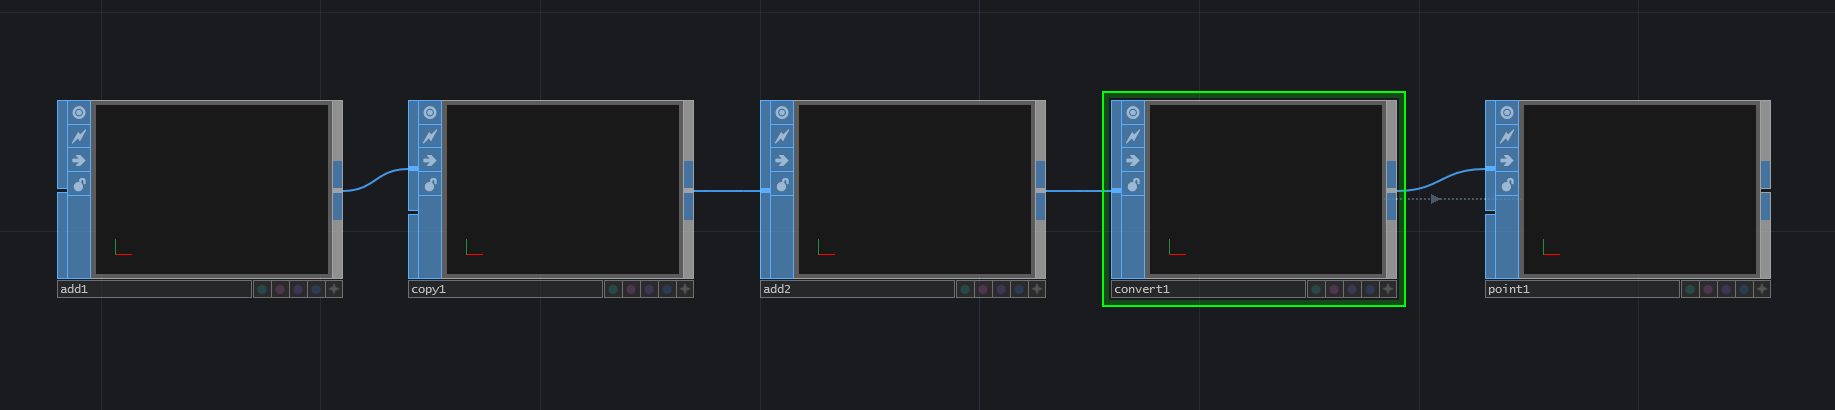
\includegraphics{./img/12.6.2/step1_2.png}
\end{center}

The next thing we're going to do is create some noise that we will use as our point positions. The first thing to do is create a 'Noise TOP'. In the 'Common' parameters, change the resolution to 1000 pixels by 1 pixels and the 'Pixel Format' to '32-bit float (RGBA)'. This gives us one pixel of noise for every particle we have (1000 pixels of noise for 1000 particles). Changing the 'Pixel Format' to '32-bit float (RGBA)' means that every pixel will have 32-bits per color channel, meaning a lot more precise data can be held in each color channel. The next step is to set the 'Monochrome' parameter to 'off'. This returns a different noise value for each of the color channels, which will be translated into different noise values for our X,Y,Z positions of the particles. You can then choose to animate the noise however you like for the example, but the easiest is the add the following code to the 'Translate' parameter's 'tx' value:

\begin{lstlisting}
absTime.frame/100
\end{lstlisting}

This will transform the noise along the X axis, which will create a ribbon-effect on the initial particle system. Next we're going to create a 'GLSL TOP' that will allow us to have more fine tuned control over the current noise values in each color channel. We'll be able to scale those values, and then in further sections, expand on the same shader to add more functionality. Connect the output of the 'Noise TOP' to the first input of a 'GLSL TOP'. The 'GLSL TOP' is created by default with a 'Text DAT' docked to it, with a default shader that outputs the color white. Edit the 'Text DAT', erase the existing code, add the code below, and then save it:

\begin{lstlisting}
out vec4 fragColor;

void main()
{
// sample the input
vec4 inPosition = texture(sTD2DInputs[0], vUV.st);

// scale each color channel (the XYZ of the vector) separately
vec4 outPosition = vec4(inPosition.x * 5.0 - 2.5, inPosition.y * 5.0 - 2.5, inPosition.z * -5.0 - 20.0, 1.0);

// output the new position
fragColor = outPosition;
}
\end{lstlisting}

We'll quickly review the code above, but please refer to previous sections in this chapter. We first setup the main output 'fragColor'. We then sample the texture at the current UV. Because we setup the 'Noise TOP' to have the sample number of pixels as there are particles, then we can sample the pixels on a one to one basis for each particle. After we sample the current pixel, we scale the R and G channels (the X and Y of the vec4) by 5.0 and then translate them 2.5 units to the left and down of the camera. We then we scale the B channel (the Z of the vec4) by -5.0, and then translate it 20 units away from the camera to fit the whole particle system in the scene. We can leave the alpha channel at 1.0 as we currently wont be using it.

After the scaling and translating, the 'outPosition' is assigned to the 'fragColor' output. If you'd like to see the positions that the particles will be receiving, you can connect the 'GLSL TOP' to a 'TOP to CHOP' operator and view each color channels values. This finishes step 3 and 4 of the item list.

\begin{center}
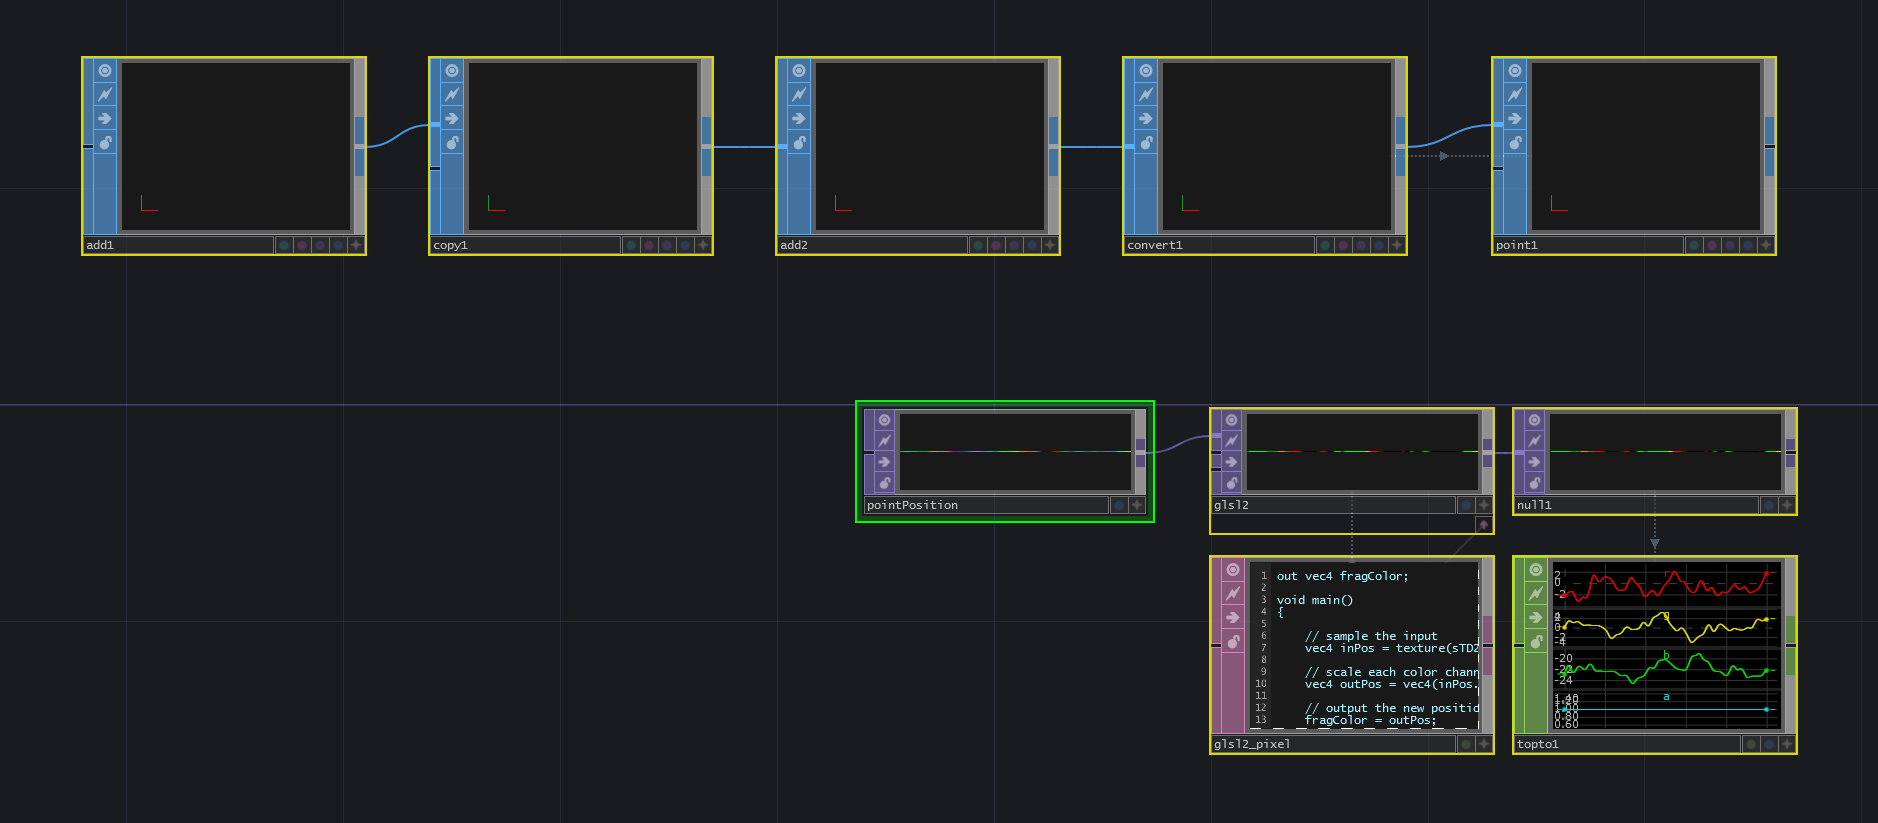
\includegraphics{./img/12.6.2/step3_4.png}
\end{center}

Now create a basic render setup by adding a 'Camera COMP', a 'Light COMP', a 'Geometry COMP', and a 'Render TOP'. They can all be set to their default values for this exercise. Make sure to add an 'In SOP' to the 'Geometry COMP' so that you can input your set of points and turn on the render and display flags on the 'In SOP' inside of the 'Geometry COMP'. That will complete step 5.

\begin{center}
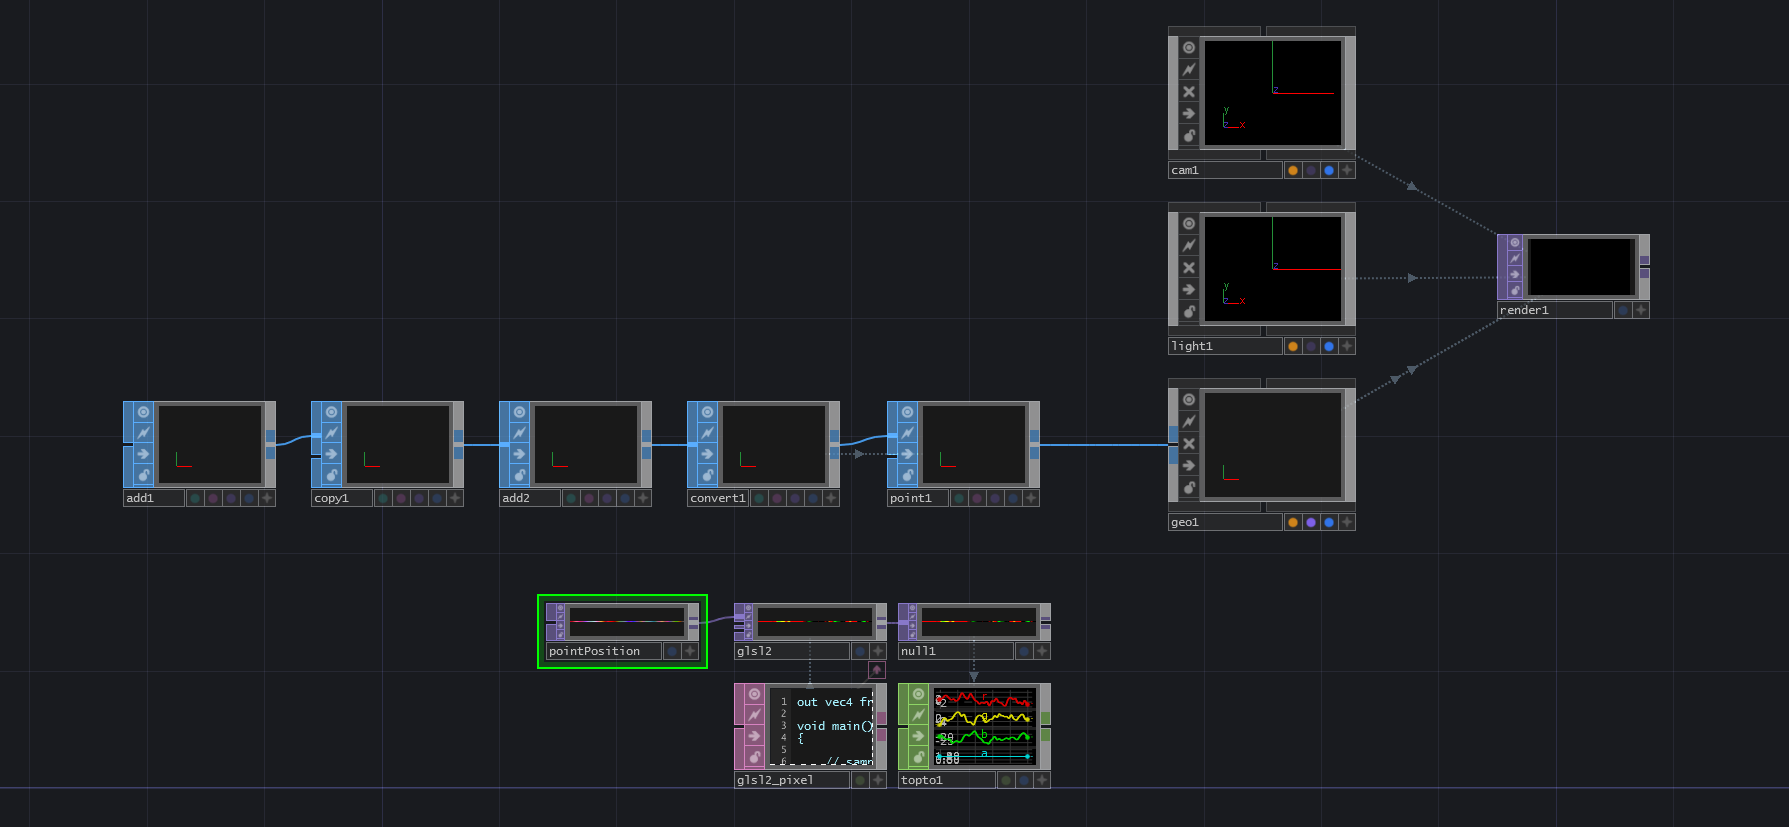
\includegraphics{./img/12.6.2/step5.png}
\end{center}

Next, create a 'GLSL MAT' operator, an 'Info DAT', and two 'Text DAT''s. Reference the 'GLSL MAT' in the 'Info DAT''s 'Operator' parameter to help debug any errors. Name one of the 'Text DAT''s 'vertex' and the other 'pixel'. These will be the GLSL vertex and pixel shaders. Reference 'vertex' in the 'GLSL MAT''s 'Vertex Shader' parameter, and reference 'pixel' in the 'GLSL MAT''s 'Pixel Shader' parameter. Then we need to reference the 'GLSL TOP' we created. To do so, on the 'Samplers 1' parameter page of the 'GLSL MAT', add 'sPointPosition' to the first 'Sampler Name' parameter, and add the name of the noise texture to the first 'TOP' parameter. In the example file, a 'Null TOP' named 'null1' was added after the 'GLSL TOP', and that is the operator name that is referenced in the 'TOP' parameter. Be very careful with the 'Sampler Name' parameter, as this will the name used in the code and if it is different than the code, you won't see any outputs as you won't be able to reference the particle position. Finally, on the 'Vectors 1' page of the 'GLSL MAT', add 'uPointsPerInstance' to the first 'Uniform Name', and enter '1.0 / 1000' as the first value of the parameter 'value0x'. This last vector will be used in the shader to scale the point index from 0-1000 to the normalized 0.0 to 1.0 UV co-ordinate when sampling the point position noise texture. With that setup complete, we can move from step 6 to step 7.

\begin{center}
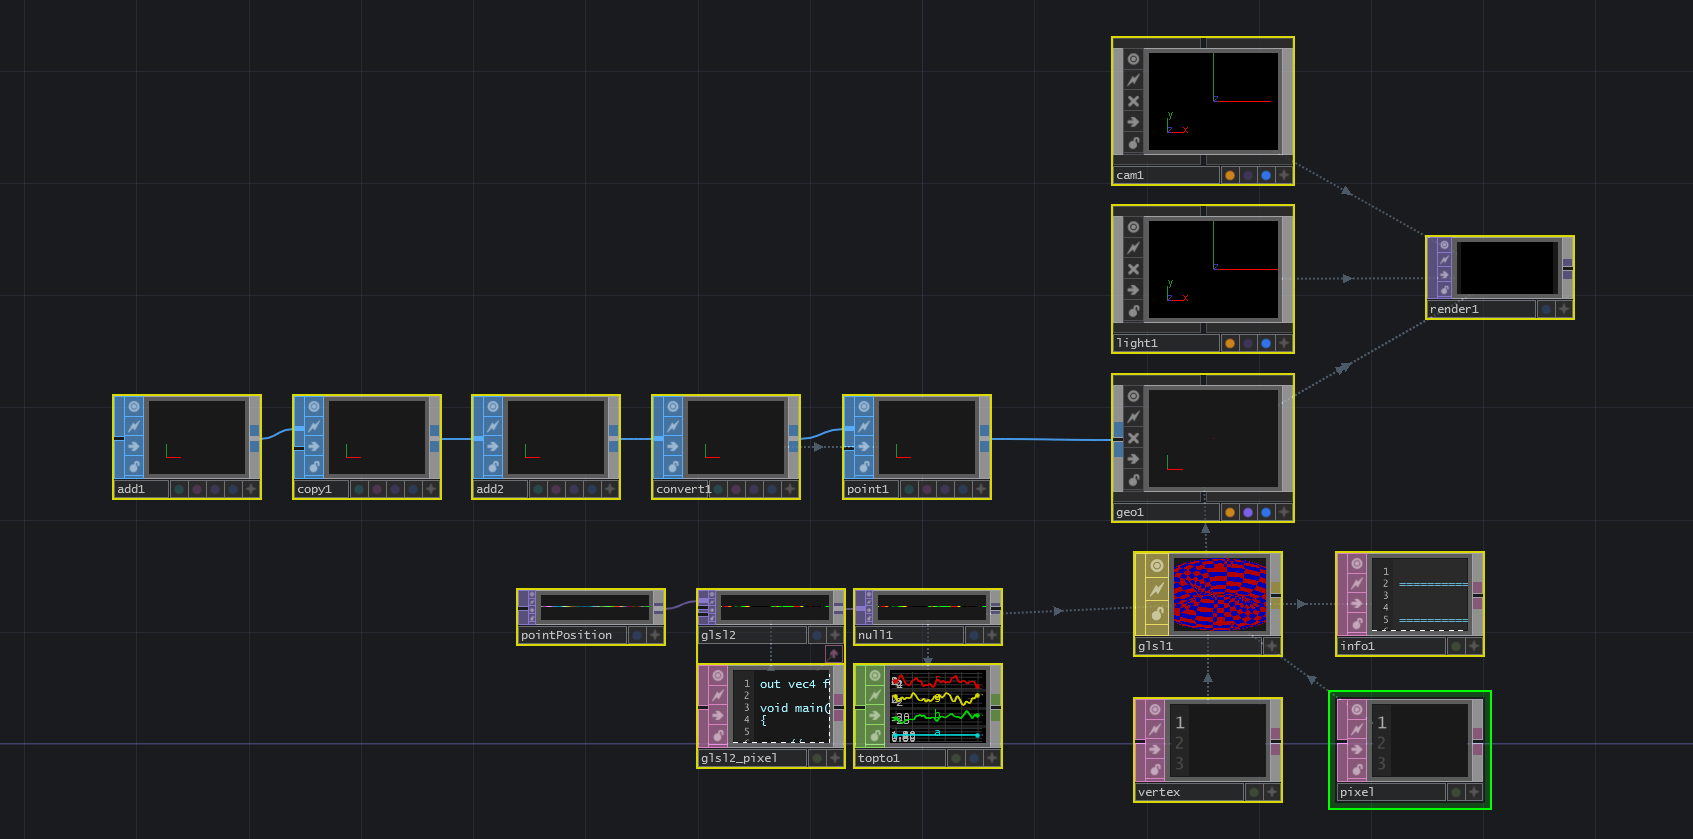
\includegraphics{./img/12.6.2/step6.png}
\end{center}

From here, we will finish all the remaining steps in the GLSL shaders. First, edit 'pixel', the 'Text DAT' we will use to hold the pixel shader, and enter the follow:

\begin{lstlisting}
layout(location = 0) out vec4 fragColor;

void main()
{
// shade pixel white
fragColor = vec4(1.0, 1.0, 1.0, 1.0);
}
\end{lstlisting}

This is a very basic pixel shader as we've seen earlier in the chapter, and all it does is shade any incoming pixels white. This completes step 7.

Edit 'vertex', the 'Text DAT' we will use to hold the vertex shader and enter the following:

\begin{lstlisting}
// setup inputs
uniform sampler2D sPointPosition;
uniform float uPointsPerInstance;
in float pointIndex;

void main()
{
    // create the uv from point index
    vec2 uv;
    uv.x = (pointIndex * uPointsPerInstance) + (uPointsPerInstance * 0.5);
    uv.y = 0.5;

    // sample the noise texture using the uv
    vec4 newPosition = texture(sPointPosition, uv);

    // set point size to your liking
    gl_PointSize = 1.0;

    // move point from object space to screen space and output to gl_Position
    vec4 worldSpaceVert = TDDeform(newPosition);
    vec4 camSpaceVert = uTDMat.cam * worldSpaceVert;
    gl_Position = TDCamToProj(camSpaceVert);
}
\end{lstlisting}

Once you enter and save that code, you will see the particle system creating a ribbon-effect using the generated noise. Let's go through this vertex shader.

The first 4 lines setup the noise texture as a 'uniform sampler2D', the 'uPointsPerInstance' value as a 'uniform float', and the incoming point index attribute as an incoming float:

\begin{lstlisting}
// setup inputs
uniform sampler2D sPointPosition;
uniform float uPointsPerInstance;
in float pointIndex;
\end{lstlisting}

The next few lines in the code create the UV to use when sampling the noise texture. To create the X location of the UV, we first take the incoming point index and multiply it by 'uPointsPerInstance', which is 1 / 1000. This gives us the location to sample from the 0.0 to 1.0 range. A key thing to remember when creating UV's manually is that the UV co-ordinates have infinite precision, so a UV of 0 along the X axis isn't the first pixel, it is the left edge of the first pixel, which will cause visual errors as the shader will then interpolate 50\% of the first pixel and 50\% of whatever is to the left of the first pixel (depending on the repeat parameters set). Because of this, we need to offset our sample by half of the sample step 'uPointsPerInstance', which is why we add the result of 'uPointsPerInstance' multiplied by 0.5 to the location we calculated by multiplying 'pointIndex' and 'uPointsPerInstance'.

To recap that:
\begin{enumerate}
\item We need to convert the point index from 0 - 1000 to the UV co-ordinates 0.0 to 1.0
\item Do that by multiplying the point index by the result of 1 / 1000, which gives us our sample step along the 0.0 to 1.0 range
\item Then add half of 'uPointsPerInstance' value (which is half of a single sample step) to offset our sampling so that we are samlping the middle of each pixel and not the left most edge
\end{enumerate}

Finally, because we know the texture is only 1 pixel tall, we can set 'uv.y' to 0.5 (again, because we don't want to sample the edge of the pixel, we want to sample the midle of it).

\begin{lstlisting}
// create the uv from point index
vec2 uv;
uv.x = (pointIndex * uPointsPerInstance) + (uPointsPerInstance * 0.5);
uv.y = 0.5;
\end{lstlisting}

The next thing to do is use the UV co-ordinates to sample the noise texture:

\begin{lstlisting}
// sample the noise texture using the uv
vec4 newPosition = texture(sPointPosition, uv);
\end{lstlisting}

Before we finish assigning the new point position, we use this handy piece of GLSL code to quickly adjust the size of the particles. We're able to do this because earlier, we used the 'Convert SOP' to set the particle types to sprites (as this code only works with sprites).

\begin{lstlisting}
// set point size to your liking
gl_PointSize = 1.0;
\end{lstlisting}

Finally, the code below takes our 'newPosition' values from object space, uses 'TDDeform()' to move them to world space. It then multiplies the position by 'uTDMat.cam' to move the point into camera space. And finally, 'TDCamToProj()' is used to convert the camera space point to screen space points, which are assigned to 'gl\_Position', which is the built-in output for each points position.

\begin{lstlisting}
// move point from object space to screen space and output to gl_Position
vec4 worldSpaceVert = TDDeform(newPosition);
vec4 camSpaceVert = uTDMat.cam * worldSpaceVert;
gl_Position = TDCamToProj(camSpaceVert);
\end{lstlisting}

With that, we've finished the first goal, which was to move particles with textures. Although this may not seem like a traditional particle system, these steps lay the foundation for the next implementations.

\begin{center}
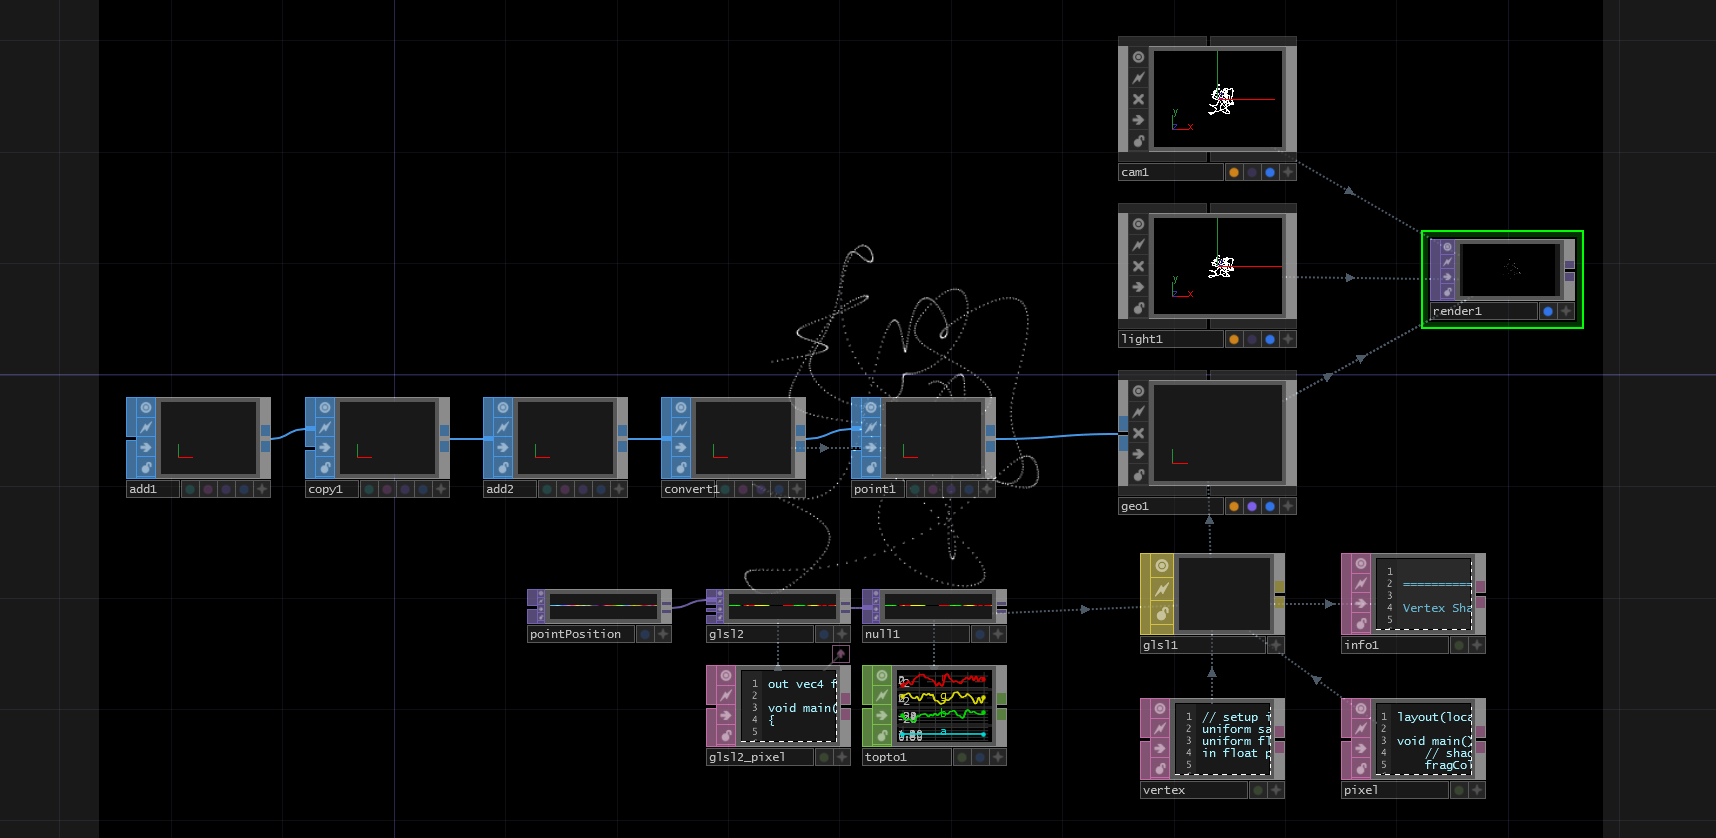
\includegraphics{./img/12.6.2/final_step.png}
\end{center}


\end{fullwidth}


\subsection{Using Source Geometry}
\begin{fullwidth}
Now that we have a basic grasp on moving particles using textures, we can add in a piece of geometry and use its positions as starting positions for our particle system. In this exercise, we'll replace our 'Add SOP' with a 'Grid SOP' (with the same point count) and add some noise to each particle position. These are the steps we will follow:

\begin{enumerate}
\item Create a texture from the point position data of 'Grid SOP'
\item Use this texture to position our particles in the point positions of the 'Grid SOP'
\item Apply the previous noise texture on the new positions to create an effected grid
\end{enumerate}

It is best to read this text while examing the example project '02\_Source\_geometry.toe', because I will refer to certain operators by their names in the example project.

The first step is to create a texture from the point position data of the 'Grid SOP'. The source of point positions in the first example was an 'Add SOP', a 'Copy SOP', and another 'Add SOP'. Start by removing these and replacing them with a 'Grid SOP' with the 'Rows' parameter set to 100 and the 'Columns' parameter set to 10. This combination of rows and columns will create a grid with the same number of points as our previous example.

The next step is to get all the point positions from the 'Grid SOP' using a 'SOP to CHOP'. Create a 'SOP to CHOP' and set the 'SOP' parameter to the name of the 'Grid SOP' which in this case is 'grid1'.

This creates a CHOP with all the point positions as separate channels. We can translate these XYZ channels into RGB channels of a texture by using the 'CHOP to TOP'. Create a 'CHOP to TOP' and set the 'CHOP' parameter to the name of the 'SOP to CHOP', which in this example is 'sopto1'. Make sure the set the 'Pixel Format' to '32-bit float (RGBA)' in the 'Common' settings of the 'CHOP to TOP', as we will be feeding this into the GLSL shader and want it to continue outputting a 32-bit texture. Connect the output of the 'CHOP to TOP' to the second input of 'glsl2', the 'GLSL TOP' we were using in the last example to scale the noise values.

This complete the first step of the example.

\begin{center}
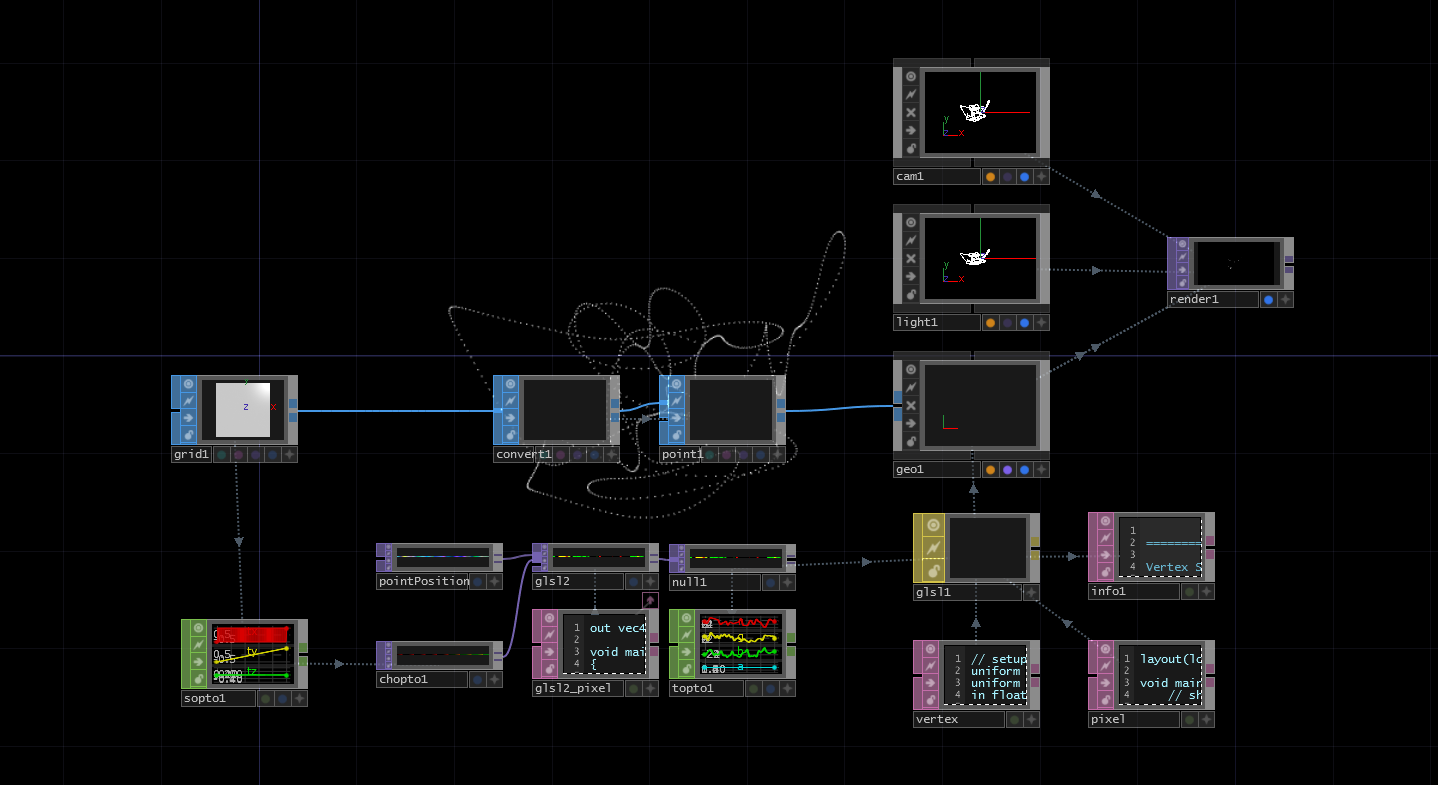
\includegraphics{./img/12.6.3/step1.png}
\end{center}

Now that we have a texture, let's make a few additions to our shader. Below is our final shader from the previous example:

\begin{lstlisting}
out vec4 fragColor;

void main()
{
// sample the input
vec4 inPosition = texture(sTD2DInputs[0], vUV.st);

// scale each color channel (the XYZ of the vector) separately
vec4 outPosition = vec4(inPosition.x * 5.0 - 2.5, inPosition.y * 5.0 - 2.5, inPosition.z * -5.0 - 20.0, 1.0);

// output the new position
fragColor = outPosition;
}
\end{lstlisting}

We'll start by adding a line to sample the new texture with the 'Grid SOP' position data. Insert this line after line 7 (we will review the full code at the end):

\begin{lstlisting}
vec4 gridPosition = texture(sTD2DInputs[1], vUV.st);
\end{lstlisting}

This creates a new 4-part vector with our XYZ data that is connected to the second input (remember the inputs are indexed starting at 0). If you'd like to visualize this very quickly, change the last line temporarily to:

\begin{lstlisting}
fragColor = gridPosition;
\end{lstlisting}

This will move all of the particles to the static points on the 'Grid SOP'. Before continuing, make sure the change the final line back to:

\begin{lstlisting}
fragColor = outPosition;
\end{lstlisting}

Now we're going to focus on this line:

\begin{lstlisting}
vec4 outPosition = vec4(inPosition.x * 5.0 - 2.5, inPosition.y * 5.0 - 2.5, inPosition.z * -5.0 - 20.0, 1.0);
\end{lstlisting}

Previously, we were taking the noise values, scaling them to make them interesting, then offsetting them to sit nicely in the camera's view. Our goal now is to take the incoming grid positions, and effect them with the noise. To do so, we can use a line like this:

\begin{lstlisting}
vec4 outPosition = vec4(gridPosition.x + (inPosition.x * 0.1), gridPosition.y + (inPosition.y * 0.1), gridPosition.z + inPosition.z, 1.0);
\end{lstlisting}

Inside each part of the 'vec4', we're taking the 'Grid SOP' XYZ and adding to it the XYZ of the noise texture. The only extra thing we've added here, is that before adding the X and Y values of the noise, we're scaling them down, as it makes it a bit easier to see the 'Grid SOP' shape in the render. The full shader code should look like this:

\begin{lstlisting}
out vec4 fragColor;

void main()
{
// sample the inputs
vec4 inPosition = texture(sTD2DInputs[0], vUV.st);
vec4 gridPosition = texture(sTD2DInputs[1], vUV.st);

// add scaled noise texture values to the grid position values
vec4 outPosition = vec4(gridPosition.x + (inPosition.x * 0.1), gridPosition.y + (inPosition.y * 0.1), gridPosition.z + inPosition.z, 1.0);

// output the new position
fragColor = outPosition;
}
\end{lstlisting}


Once you save, you should the columns of the grid being effected by the noise texture.

\begin{center}
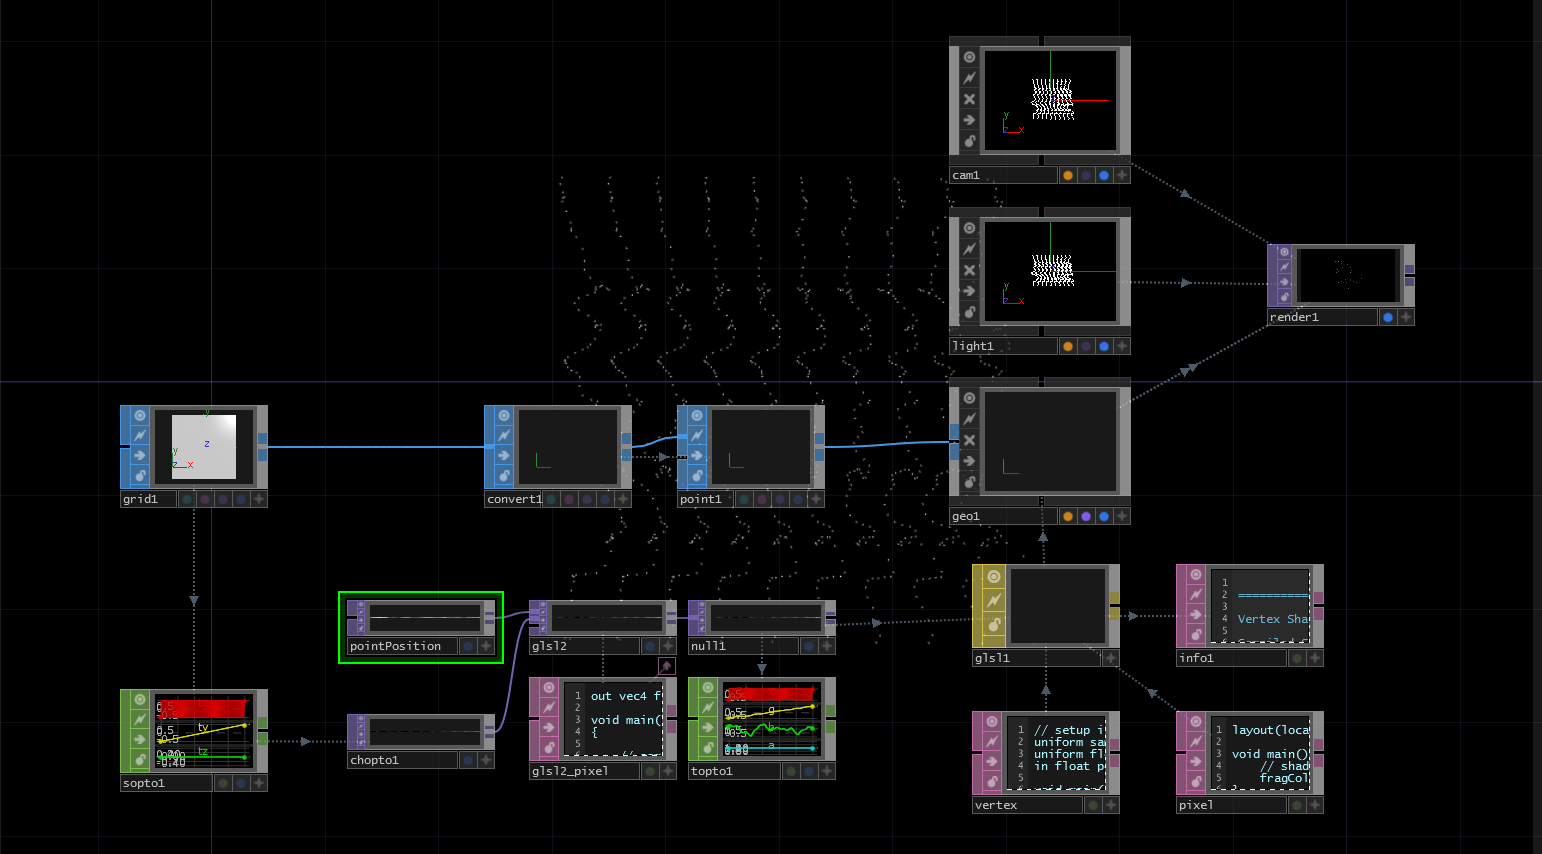
\includegraphics{./img/12.6.3/step2_3.png}
\end{center}

Feel free to experiment by replacing the 'Grid SOP' with another geometry with 1000 points.

\end{fullwidth}
%------------------------------------------------
\section{What Next?}
\begin{fullwidth}
This chapter should have helped unravel a bit of the introductory mysteries of GLSL without getting unnecessarily technical.

If you'd like to continue learning GLSL to experiment with more complex 3D scenes and material shaders, or with more complex 2D compositing tools and generative textures, below are some resources:

\begin{enumerate}
\item OpenGL Main reference page: \url{http://www.opengl.org/wiki/Main_Page}
\item OpenGL General information: \url{http://www.opengl.org/wiki/General_OpenGL}
\item Derivative Wiki: \url{http://www.derivative.ca/wiki088/index.php?title=Glsl}
\item Shader Toy: \url{https://www.shadertoy.com/}
\end{enumerate}
\end{fullwidth}


%----------------------------------------------------------------------------------------
% CHAPTER 13
%----------------------------------------------------------------------------------------

\cleardoublepage
\chapter{Projects}
\label{ch:13}

%------------------------------------------------

\begin{fullwidth}

This section will revolve around materials that are outside of the book itself. In the 'Projects' folder, there are two subfolders - 'Beginner' and 'Advanced'. Each will house a series of tutorials that include project files and videos. 

Some of these projects will be technical in nature, some will be artistic, but all of them will try to highlight a concept or common task.

The videos will start from a blank slate and build the project to completion, highlighting the problem solving approaches taken to complete the project.

\end{fullwidth}

%------------------------------------------------



%----------------------------------------------------------------------------------------
% CHAPTER 14
%----------------------------------------------------------------------------------------

\cleardoublepage
\chapter{Credits}
\label{ch:14}

%------------------------------------------------

\begin{fullwidth}

\textit{In order of contribution:}

Elburz Sorkhabi - original author \& creator, editor

\end{fullwidth}

%------------------------------------------------



%----------------------------------------------------------------------------------------

\end{document}